%% estilo do documento e medidas
\documentclass[a4paper,portuguese,utf8,T1]{article}
\usepackage[top=3cm,bottom=2cm,left=2cm,right=2cm,marginparwidth=1.75cm]{geometry}
\usepackage{indentfirst}
\renewcommand{\baselinestretch}{1.2}
\setlength{\marginparwidth}{2cm}

%% linguagem e fontes
\usepackage[utf8]{inputenc}
\usepackage[T1]{fontenc}
\usepackage[portuguese]{babel}

%% referencias
\usepackage[
    backend = biber,
    style = alphabetic,
    sorting = ynt
]{biblatex}
\addbibresource{dados/referencias.bib}

%% pacotes para desenhos e ambientes diferenciadas
\usepackage{amsmath}						% símbolos e ambientes matemáticos
\usepackage{booktabs}						% tabelas melhoradas
\usepackage{datatool}						% recolhimento de dados
\usepackage[table,xcdraw]{xcolor}			% mais cores
\usepackage{graphicx}						% figuras melhoradas
\usepackage{subcaption}						% subfiguras
\usepackage[colorinlistoftodos]{todonotes}	% notas para a escrita
\usepackage[colorlinks,citecolor=blue]{hyperref}		% links
\usepackage{circuitikz}						% desenho de circuitos
\usepackage{csvsimple}						% dados em CSV
\usepackage{cleveref}						% referenciamento melhorado
\usepackage{multirow}						% tabelas de multíplas linhas ou colunas
\usepackage{float}							% fixar posição de figuras
\usepackage{csquotes}                       % aspas melhoradas
\usepackage{textcomp}
\usepackage{gensymb}
\usepackage{amssymb}
\usepackage{titling}
\usepackage{mhchem}

% unidades do SI
\usepackage[
	exponent-to-prefix = true,
	round-mode = figures,
	scientific-notation = engineering,
	zero-decimal-to-integer = false,
	separate-uncertainty = true,
	multi-part-units = single
]{siunitx}

% setup para usar o cleveref com o subcaption
% \captionsetup[subfigure]{subrefformat=simple,labelformat=simple}
%     \renewcommand\thesubfigure{(\alph{subfigure})}

%% dados do relatório
\def\svgwidth{.25\columnwidth}
\pretitle{
	\begin{center}
	\Huge
	%% Creator: Inkscape inkscape 0.92.2, www.inkscape.org
%% PDF/EPS/PS + LaTeX output extension by Johan Engelen, 2010
%% Accompanies image file 'IFGW.pdf' (pdf, eps, ps)
%%
%% To include the image in your LaTeX document, write
%%   \input{<filename>.pdf_tex}
%%  instead of
%%   \includegraphics{<filename>.pdf}
%% To scale the image, write
%%   \def\svgwidth{<desired width>}
%%   \input{<filename>.pdf_tex}
%%  instead of
%%   \includegraphics[width=<desired width>]{<filename>.pdf}
%%
%% Images with a different path to the parent latex file can
%% be accessed with the `import' package (which may need to be
%% installed) using
%%   \usepackage{import}
%% in the preamble, and then including the image with
%%   \import{<path to file>}{<filename>.pdf_tex}
%% Alternatively, one can specify
%%   \graphicspath{{<path to file>/}}
%%
%% For more information, please see info/svg-inkscape on CTAN:
%%   http://tug.ctan.org/tex-archive/info/svg-inkscape
%%
\begingroup%
  \makeatletter%
  \providecommand\color[2][]{%
    \errmessage{(Inkscape) Color is used for the text in Inkscape, but the package 'color.sty' is not loaded}%
    \renewcommand\color[2][]{}%
  }%
  \providecommand\transparent[1]{%
    \errmessage{(Inkscape) Transparency is used (non-zero) for the text in Inkscape, but the package 'transparent.sty' is not loaded}%
    \renewcommand\transparent[1]{}%
  }%
  \providecommand\rotatebox[2]{#2}%
  \newcommand*\fsize{\dimexpr\f@size pt\relax}%
  \newcommand*\lineheight[1]{\fontsize{\fsize}{#1\fsize}\selectfont}%
  \ifx\svgwidth\undefined%
    \setlength{\unitlength}{174.60993718bp}%
    \ifx\svgscale\undefined%
      \relax%
    \else%
      \setlength{\unitlength}{\unitlength * \real{\svgscale}}%
    \fi%
  \else%
    \setlength{\unitlength}{\svgwidth}%
  \fi%
  \global\let\svgwidth\undefined%
  \global\let\svgscale\undefined%
  \makeatother%
  \begin{picture}(1,0.47769889)%
    \lineheight{1}%
    \setlength\tabcolsep{0pt}%
    \put(0,0){
\includegraphics[width=\unitlength,page=1]{figuras/logo/IFGW.pdf}}%
  \end{picture}%
\endgroup%

	\\[\bigskipamount]
}
\posttitle{
	\end{center}
}
\title{
	Experimento 4 			\\
    \Large Física Experimental IV
}
\author{
	\small Grupo 3:					\\
	Felipe Mack (81335),			\\
    Gabriel Ferrauche (197314) e	\\
    Tiago de Paula (187679)
}
\date{\small\today}

%%%%%%%%%%%%%%%%%%%%%%%%%%%%%
%% Relatório, propriamente %%
%%%%%%%%%%%%%%%%%%%%%%%%%%%%%
\begin{document}

	%% Cabeçalho %%
	\maketitle

	%%%% Resumo %%%%
	\begin{abstract}
    	\textit{\textit{Neste experimento foi estudado o potencial de uso de circuitos RC como integradores e diferenciadores de um sinal de entrada. Além disso, também foi feito o estudo do fenômeno transiente e de oscilações forçadas amortecidas em um filtro ressonante, em regimes sub-amortecido e sobre amortecido, com o sinal de saída estabilizando-se ao redor do sinal de entrada. Ao final, verificou-se que filtros passivos de um componente reativo podem atuar convenientemente como operadores de diferenciação e integração e que oscilações em um circuito analógico ocorrem de forma altamente similar a outros sistemas oscilatórios}}
	\end{abstract}

	%%%%% Introdução %%%%%
	\section{Introdução} \label{introducao}
		Em sistemas de controle, é de suma importância monitorar como certas grandezas físicas se comportam com o passar do tempo. Para tal observação, analisar tanto a derivada quanto a integral dessas grandezas mostra-se extremamente importante. em eletrônica analógica, a forma mais comum de cumprir esta tarefa é empregando circuitos diferenciadores e integradores.

A forma mais comum de se construir os circuitos supracitados é empregando filtros passivos de um componente reativo, ou seja, filtros RC e RL. Ao observar circuitos desse tipo em relação ao domínio de tempo, dadas frequências especificas, o sinal de saída desses sistemas é capaz de representar a derivada ou integral do sinal de entrada e assim, possibilitando seu monitoramento.

Muitos sistemas físicos apresentam comportamento oscilatório. Filtros RLC, os chamados filtros ressonantes, também  exibem o mesmo tipo de comportamento. Dessa forma, observar como os mesmo se comportam durante as oscilações é útil para estudar como esse fenômeno ocorre.

Considerando os sistemas citados, o objetivo deste experimento é construir um circuito capaz de integrar sinais arbitrários com frequências maiores que $\SI{50}{\kilo\hertz}$ e diferenciar sinais com frequência menos que \SI{500}{\hertz}. Além disso, também temos como objetivo estudar o fenômeno transiente utilizando um circuito RLC que possa operar em dois regimes de amortecimento, subamortecido e sobreamortecido, de forma que, no regime estacionário, a tensão de saída se estabilize ao redor da tensão de entrada.


	%%%%% Materiais e Métodos %%%%%
	\section{Materiais e Métodos} \label{metodos}
    	\subsection{Procedimentos experimentais}

Para as obtenção das medidas desejadas foi empregado um laser de luz verde aproximadamente monocromática ($\lambda = \SI{532}{\nano\meter}$~\cite{ref:roteiro}).

Inicialmente, foi feito o alinhamento do laser, de forma que as medições pudessem ser realizadas com precisão. Para tal, um vidro metálico contendo diversas fendas variadas (figura \ref{fig:rede}), impressas por litografia, foi alinhado perpendicularmente ao feixe do laser. Em seguida o feixe refletido foi alinhado com o feixe incidente, garantindo o alinhamento do trilho em que o vidro estava montado.

\begin{figure}[H]
	\centering	    
	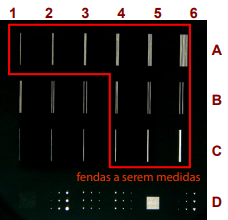
\includegraphics[scale=0.6]{figuras/rede_dif.png}
	\caption{Vidro e fendas utilizadas}
	\label{fig:rede}
\end{figure}

A fim de coletar os dados, buscando medir padrões de difração para fendas simples, o laser foi incidido na fenda C4, de forma que o padrão de difração pudesse ser observado em um papel milimetrado utilizado como anteparo. O procedimento foi repetido para as fendas C5 e C6.

Para esta situação, o modelo de difração de Fraunhofer~\cite{ref:otica} mostra que:
\begin{equation*}
    \Delta y \approx \frac{2 \lambda z}{b} \label{eq:difr}
\end{equation*}

Sendo que $\Delta y$ é a largura dos máximos da difração, $z$ a separação entre o emissor de luz e o anteparo e $\lambda$ o comprimento de onda da luz emitida. Com isso, dado que $z$ pode ser medido experimentalmente e conhecendo o comprimento de onda, é possível determinar a largura das fendas $b$, sendo este o procedimento realizado pelo grupo.

Na sequência, foram medidos os padrões para fendas duplas, B4, B5 e B6, e múltiplas, de A1 a A6, utilizando o mesmo procedimento anterior. Vale ressaltar que, para as fendas duplas, as espessuras eram iguais, enquanto, para as fendas múltiplas, as aberturas e as separações eram, nominalmente, as mesmas, mudando apenas o número de fendas.

Aplicando o modelo de Fraunhofer~\cite{ref:otica} sobre a interferência de fendas duplas, a separação entre máximos (ou mínimos) consecutivos no anteparo é dada por:
\begin{equation}
    \Lambda \approx \frac{\lambda z}{h} \label{eq:duplas}
\end{equation}

Onde que $h$ é a separação entre as fendas. Assim, de forma análoga ao processo para fendas simples, é possível determinar a separação entre as fendas a partir do comprimento de onda da luz emitida. Para determinação da largura das fendas, bastou aplicar o modelo de Fraunhofer para difração em fenda simples, já que para fendas duplas o fenômeno de difração também ocorre juntamente com interferência.

Já para uma quantidade generalizada $N$ de fendas, a análise muda e passamos a pensar na largura dos máximos primários $\delta\gamma$, que é aproximadamente metade da largura da base e é dada por:
\begin{equation}
    \delta y \approx \delta\gamma = \frac{\lambda z}{N h} \label{eq:mult}
\end{equation}

Em que $\delta y$ é a metade da largura da base dos máximos primários. Nota-se, também, que essa equação engloba o caso de fendas duplas, já que no caso específico de $N = 2$, teremos $\Lambda = 2 \delta y \approx 2 \frac{\lambda z}{2 h} = \lambda z / h$

As fendas múltiplas de mesma separação (A2-A6) também foram utilizadas para comprovar a relação: $$\delta y \propto \frac{1}{N} \label{rel:dyn}$$ Para tanto, montou-se um gráfico log-log de $\delta y \times N$ e, então, foi feita uma regressão linear do tipo $\log(\delta y) = A + B \log(N)$. Com essa regressão, $B$ se torna o expoente de $N$ na relação acima. A regressão foi seguindo o recomendado no Guia de Incertezas~\cite{ref:gum}, bem como as incertezas de cada coeficiente.

A próxima etapa do experimento consistia da observação de padrões de difração com a luz incidindo em um fio de cabelo, onde foi utilizado um pequeno quadro de material plástico, de tamanho similar ao vidro utilizado anteriormente, com o fio de cabelo fixado em seu centro (figura \ref{fig:fiocab}). A luz foi incidida no feixe e o padrão gerado foi observado no anteparo. É importante notar que, de acordo com o Princípio de Babinet~\cite{ref:wolf}, o modelo de Fraunhofer para fendas simples é aplicável para este padrão de difração, fazendo com que a determinação da largura do fio de cabelo seja análoga a determinação da largura de uma fenda simples.

\begin{figure}[H]
	\centering
	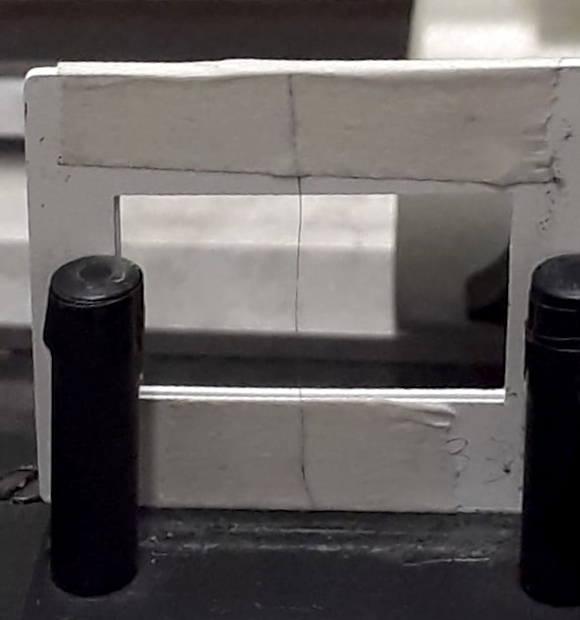
\includegraphics[scale=1.6]{figuras/mcabelo.jpg}
	\caption{Fio de cabelo utilizado}
	\label{fig:fiocab}
\end{figure}

A última etapa de observações foi feita analisando os padrões de difração em aberturas variadas, em geral, não sendo fendas. O mesmo procedimento citado anteriormente foi realizado para as aberturas D, com intuito de inferir o formato presente em cada uma.

Durante todos os procedimentos descritos anteriormente, fotos do anteparo foram tiradas utilizando um celular, a fim de analisar os padrões formados utilizando o \textit{software} \texttt{ImageJ}\cite{ref:imagej}. Assim possibilitando a determinação das distâncias dos mínimos de difração ($\Delta y$), dos máximos de interferência ($\Lambda$) e a largura da base dos máximos primários ($2 \delta y$). Além disso, o grupo determinou que a resolução do papel e a medição do distanciamento do anteparo foram as principais fontes de incerteza a serem consideradas. Vale citar que outras fontes de incerteza, como o posicionamento (paralaxe) e resolução da câmera também foram identificadas apesar de não serem consideradas durante o processamento dos dados, pois se tratavam de incertezas de difícil abordagem e buscou-se minimizá-las durante a coleta de dados.

Por fim, utilizando um microscópio metrológico, foram medidas as larguras das fendas ($b$), a separação entre elas ($h$) e a quantidade de fendas ($N$), em todas as situações anteriores. Também foram evitadas medições repetidas com esse equipamento, no caso, as separações e as larguras das fendas da linha A, que eram iguais. Para a utilização desse microscópio,foram identificadas como incertezas sua resolução e paralaxe na leitura.

\subsection{Incertezas}
    Começando pela incerteza das medidas dimensionais do experimento, a trena usada para medir a distância $z$ da fenda ao anteparo (papel milimetrado). Como são medições analógicas, considerou-se uma distribuição triangular, fazendo a incerteza da medição ser:
\begin{equation*}
    u_\text{medição} = \text{resolução} \times \frac{\sqrt{6}}{12}
\end{equation*}

Também assumiu-se uma incerteza de calibração de posicionamento da trena, como a incerteza de medição do ponto \SI{0}{\centi\meter}. Esta incerteza poderia ser determinada de forma idêntica à anterior, dessa forma, $u_\text{calibração} = u_\text{medição}$. A incerteza total então seria:
\begin{align*}
    u_\text{total}
        &= \sqrt{u_\text{calibração}^2 + u_\text{medição}^2} \\
        &= u_\text{medição} \sqrt{2} \\
        &= \text{resolução} \times \frac{\sqrt{3}}{6}
\end{align*}

Já para o caso do papel milimetrado do anteparo, esse tipo de incerteza não é aplicável, porém, como a medição é dada por dois pontos, teremos duas incertezas $u_\text{medição}$, o que torna a incerteza total igual a da trena. Um ponto a expor sobre essa medida é que ela é encontrada a partir de duas dimensões, o que complica os cálculos da incerteza. Porém, esse valor é encontrado pelo \texttt{ImageJ}\cite{ref:imagej}, onde o resultado é bem mais preciso, o que deixa válida a assunção de que possa ser considerada apenas a incerteza de uma das dimensões.

Para ambos os casos anteriores $\text{resolução} = \SI{1}{\milli\meter}$, e, então, $u_\text{total} = \SI{.3}{\milli\meter}$. Dentre as medidas calculadas desta maneira, é importante lembrar do valor de $z$ e sua incerteza, a qual determinou-se $\Delta z = \SI{.3}{\milli\meter}$.

Agora, para os valores calculados a partir do modelo de difração de Fraunhofer, foram feitas as devidas propagações de incertezas, tendo como referência o padrão do INMETRO, o GUM\cite{ref:gum}. O primeiro desses valores é o $b$, da equação \ref{eq:difr}, cujas derivadas parciais são:
\begin{gather*}
    \frac{\partial b}{\partial z} = \frac{2 \lambda}{\Delta y} \\
    \frac{\partial b}{\partial \lambda} = \frac{2 z}{\Delta y} \\
    \frac{\partial b}{\partial (\Delta y)} = -\frac{2 \lambda z}{(\Delta y)^2}
\end{gather*}

Porém, como não existe uma incerteza associada a $\lambda$, tem-se:
\begin{align*}
    \Delta b
        &= \sqrt{\left(\frac{\partial b}{\partial z}\right)^2 (\Delta z)^2 + \left(\frac{\partial b}{\partial (\Delta y)}\right)^2 (\Delta (\Delta y))^2} \\
        &= \frac{2 \lambda}{\Delta y} \sqrt{(\Delta z)^2 + z^2 \left(\frac{\Delta (\Delta y)}{\Delta y}\right)^2}
\end{align*}

Também faz parte do procedimento experimental a redução numérica da incerteza. Dessa forma, é importante o cálculo de $n_y$ máximos, em vez de apenas um. Assim, a medida passa a ser $n_y \Delta y$, com a mesma incerteza do $\Delta y$ original. A nova incerteza então passar a ser:
\begin{equation*}
    \Delta (\Delta y) = \frac{\Delta (n_y \Delta y)}{n_y} = \frac{u_\text{total}}{n_y}
\end{equation*}

Com um processo bem similar foi aplicado na separação $h$ das fendas duplas, pela eq. \ref{eq:duplas}, chega-se em:
\begin{equation*}
    \Delta h = \frac{\lambda}{\Lambda} \sqrt{(\Delta z)^2 + z^2 \left(\frac{\Delta \Lambda}{\Lambda}\right)^2}
\end{equation*}

Aplicando o mesmo processo de redução da incerteza, isto é, medindo $n_\Lambda \Lambda$, no lugar de somente $\Lambda$, a incerteza reduz para $\Delta \Lambda = u_\text{total}/n_\Lambda$ também.

Para a separação de múltiplas fendas (eq. \ref{eq:mult}), a propagação é novamente muito similar, resultando em:
\begin{equation*}
    \Delta h = \frac{\lambda}{N \delta y} \sqrt{(\Delta z)^2 + z^2 \left(\frac{\Delta \delta y}{\delta y}\right)^2}
\end{equation*}

Nesse caso, no entanto, a redução de incerteza usada anteriormente não é aplicável.

Para a medida final, com o microscópio metrológico, voltam as incertezas de medidas experimentais. A incerteza de leitura é similar àquela usada na trena, porém julgou-se necessário considerar uma incerteza de paralaxe, devido a leitura com a lupa. Tal procedimento assume uma distribuição retangular, pois pode facilmente mudar a leitura uma casa acima ou abaixo, de acordo com a posição do observador. Assim:
\begin{gather*}
    u_{\text{medição}} = \frac{\text{resolução}}{2 \sqrt{6}} = \text{resolução} \times \frac{\sqrt{6}}{12} \\
    u_{\text{paralaxe}} = \frac{2\ \text{resolução}}{2 \sqrt{3}} = \text{resolução} \times \frac{\sqrt{3}}{3} \\
    \Delta L_i = u_{\text{total}}
        = \sqrt{u_{\text{medição}}^2 + u_{\text{paralaxe}}^2}
        = \text{resolução} \times \frac{\sqrt{6}}{4}
\end{gather*}

Então, como $b = L_2 - L_1$ e $h = L_3 - L_1$:
\begin{equation*}
    \Delta b = \Delta h = \sqrt{(\Delta L_i)^2 + (\Delta L_j)^2} = u_\text{total} \sqrt{2} = \text{resolução} \times \frac{\sqrt{3}}{2}
\end{equation*}

Sendo que a resolução do equipamento é \SI{1}{\micro\meter}, a incerteza é $\Delta b = \Delta h = \SI{.9}{\micro\meter}$.



	%%%%% Resultados %%%%%
	\section{Resultados} \label{resultados}
	 	\begin{table}[H]
	\centering
	\sisetup{
        round-precision = 5,
        arc-separator = \,,
        minimum-integer-digits = 2
	}
	\begin{tabular}{cc}
		\toprule\toprule
            {\bfseries Medida} & {\bfseries Valor}
        \\\midrule
            $\theta_{L_1}$ & $\ang{56;30;00}\pm\ang{;;36}$ \\
            $\theta_{L_2}$ & $\ang{298;20;00}\pm\ang{;;36}$
        \\\midrule
            $\alpha$ & $\ang{59;05;00}\pm\ang{;;25}$
        \\\bottomrule\bottomrule
	\end{tabular}

	\caption{Medidas para o cálculo da abertura do prisma}
	\label{tab:apice}
\end{table}

As primeiras medições feitas após toda a calibração do equipamento foram do ápice do prisma, cujos valores estão detalhados na tabela \ref{tab:apice}. A partir desse valor da abertura $\alpha$ e dos desvios mínimos tabelados em \ref{tab:desvios}, foram encontrados os índices de refração do prisma para cada linha espectral (pela relação \ref{eq:n}), apresentados na mesma tabela.

\DTLloaddb{desvios}{dados/desvio.csv}

\begin{table}[H]
	\centering
	\sisetup{
		table-figures-uncertainty = 1
	}
	\begin{tabular}{cccc}
		\toprule\toprule
            {\bfseries Lâmpada}
				& {\bfseries Comprimento de onda}
                & {\bfseries Desvio mínimo}
                & {\bfseries Índice de refração}

		\DTLforeach*{desvios}{\cp=composto, \lm=lambda,\dv=dm_d,\dm=dm_m,\n=n,\nr=nr}{
			\DTLiffirstrow{\\\midrule}{\\}

			\ce{\cp}
				& \SI[round-precision = 5]{\lm}{\nano\meter}
				& $\ang[arc-separator = \,, minimum-integer-digits = 2]{\dv;\dm;00} \pm\ang{;;37}$
				& $\num[round-precision = 4]{\n}\pm\nr$
		}
        \\\bottomrule\bottomrule
	\end{tabular}

	\caption{Desvio mínimo medido para cada comprimento de onda}
	\label{tab:desvios}
\end{table}

Com isso, os últimos dados restantes vieram do roteiro do experimento~\cite{ref:roteiro}, que são os comprimentos de onda associados às linhas, permitindo a montagem do gráfico \ref{fig:reta} e os valores recolhidos da regressão (na tab. \ref{tab:regres}).

%% Creator: Matplotlib, PGF backend
%%
%% To include the figure in your LaTeX document, write
%%   \input{<filename>.pgf}
%%
%% Make sure the required packages are loaded in your preamble
%%   \usepackage{pgf}
%%
%% Figures using additional raster images can only be included by \input if
%% they are in the same directory as the main LaTeX file. For loading figures
%% from other directories you can use the `import` package
%%   \usepackage{import}
%% and then include the figures with
%%   \import{<path to file>}{<filename>.pgf}
%%
%% Matplotlib used the following preamble
%%   \usepackage[utf8]{inputenc}
%%   \usepackage[T1]{fontenc}
%%   \usepackage[portuguese]{babel}
%%   \usepackage{siunitx}
%%   \usepackage{gensymb}
%%   \usepackage{fontspec}
%%   \setmainfont{DejaVuSerif.ttf}[Path=/home/marmis/.virtualenvs/default/lib/python3.7/site-packages/matplotlib/mpl-data/fonts/ttf/]
%%   \setsansfont{arial.ttf}[Path=/usr/share/fonts/TTF/]
%%   \setmonofont{DejaVuSansMono.ttf}[Path=/home/marmis/.virtualenvs/default/lib/python3.7/site-packages/matplotlib/mpl-data/fonts/ttf/]
%%
\begingroup%
\makeatletter%
\begin{pgfpicture}%
\pgfpathrectangle{\pgfpointorigin}{\pgfqpoint{5.000000in}{3.000000in}}%
\pgfusepath{use as bounding box, clip}%
\begin{pgfscope}%
\pgfsetbuttcap%
\pgfsetmiterjoin%
\definecolor{currentfill}{rgb}{1.000000,1.000000,1.000000}%
\pgfsetfillcolor{currentfill}%
\pgfsetlinewidth{0.000000pt}%
\definecolor{currentstroke}{rgb}{1.000000,1.000000,1.000000}%
\pgfsetstrokecolor{currentstroke}%
\pgfsetdash{}{0pt}%
\pgfpathmoveto{\pgfqpoint{0.000000in}{0.000000in}}%
\pgfpathlineto{\pgfqpoint{5.000000in}{0.000000in}}%
\pgfpathlineto{\pgfqpoint{5.000000in}{3.000000in}}%
\pgfpathlineto{\pgfqpoint{0.000000in}{3.000000in}}%
\pgfpathclose%
\pgfusepath{fill}%
\end{pgfscope}%
\begin{pgfscope}%
\pgfsetbuttcap%
\pgfsetmiterjoin%
\definecolor{currentfill}{rgb}{0.917647,0.917647,0.949020}%
\pgfsetfillcolor{currentfill}%
\pgfsetlinewidth{0.000000pt}%
\definecolor{currentstroke}{rgb}{0.000000,0.000000,0.000000}%
\pgfsetstrokecolor{currentstroke}%
\pgfsetstrokeopacity{0.000000}%
\pgfsetdash{}{0pt}%
\pgfpathmoveto{\pgfqpoint{0.756811in}{0.683119in}}%
\pgfpathlineto{\pgfqpoint{4.808000in}{0.683119in}}%
\pgfpathlineto{\pgfqpoint{4.808000in}{2.666026in}}%
\pgfpathlineto{\pgfqpoint{0.756811in}{2.666026in}}%
\pgfpathclose%
\pgfusepath{fill}%
\end{pgfscope}%
\begin{pgfscope}%
\pgfpathrectangle{\pgfqpoint{0.756811in}{0.683119in}}{\pgfqpoint{4.051189in}{1.982907in}}%
\pgfusepath{clip}%
\pgfsetroundcap%
\pgfsetroundjoin%
\pgfsetlinewidth{0.803000pt}%
\definecolor{currentstroke}{rgb}{1.000000,1.000000,1.000000}%
\pgfsetstrokecolor{currentstroke}%
\pgfsetdash{}{0pt}%
\pgfpathmoveto{\pgfqpoint{1.256625in}{0.683119in}}%
\pgfpathlineto{\pgfqpoint{1.256625in}{2.666026in}}%
\pgfusepath{stroke}%
\end{pgfscope}%
\begin{pgfscope}%
\pgfsetbuttcap%
\pgfsetroundjoin%
\definecolor{currentfill}{rgb}{0.411765,0.411765,0.411765}%
\pgfsetfillcolor{currentfill}%
\pgfsetlinewidth{1.003750pt}%
\definecolor{currentstroke}{rgb}{0.411765,0.411765,0.411765}%
\pgfsetstrokecolor{currentstroke}%
\pgfsetdash{}{0pt}%
\pgfsys@defobject{currentmarker}{\pgfqpoint{0.000000in}{-0.066667in}}{\pgfqpoint{0.000000in}{0.000000in}}{%
\pgfpathmoveto{\pgfqpoint{0.000000in}{0.000000in}}%
\pgfpathlineto{\pgfqpoint{0.000000in}{-0.066667in}}%
\pgfusepath{stroke,fill}%
}%
\begin{pgfscope}%
\pgfsys@transformshift{1.256625in}{0.683119in}%
\pgfsys@useobject{currentmarker}{}%
\end{pgfscope}%
\end{pgfscope}%
\begin{pgfscope}%
\definecolor{textcolor}{rgb}{0.411765,0.411765,0.411765}%
\pgfsetstrokecolor{textcolor}%
\pgfsetfillcolor{textcolor}%
\pgftext[x=1.256625in,y=0.567841in,,top]{\color{textcolor}\rmfamily\fontsize{8.800000}{10.560000}\selectfont \(\displaystyle 2.5\)}%
\end{pgfscope}%
\begin{pgfscope}%
\pgfpathrectangle{\pgfqpoint{0.756811in}{0.683119in}}{\pgfqpoint{4.051189in}{1.982907in}}%
\pgfusepath{clip}%
\pgfsetroundcap%
\pgfsetroundjoin%
\pgfsetlinewidth{0.803000pt}%
\definecolor{currentstroke}{rgb}{1.000000,1.000000,1.000000}%
\pgfsetstrokecolor{currentstroke}%
\pgfsetdash{}{0pt}%
\pgfpathmoveto{\pgfqpoint{1.862094in}{0.683119in}}%
\pgfpathlineto{\pgfqpoint{1.862094in}{2.666026in}}%
\pgfusepath{stroke}%
\end{pgfscope}%
\begin{pgfscope}%
\pgfsetbuttcap%
\pgfsetroundjoin%
\definecolor{currentfill}{rgb}{0.411765,0.411765,0.411765}%
\pgfsetfillcolor{currentfill}%
\pgfsetlinewidth{1.003750pt}%
\definecolor{currentstroke}{rgb}{0.411765,0.411765,0.411765}%
\pgfsetstrokecolor{currentstroke}%
\pgfsetdash{}{0pt}%
\pgfsys@defobject{currentmarker}{\pgfqpoint{0.000000in}{-0.066667in}}{\pgfqpoint{0.000000in}{0.000000in}}{%
\pgfpathmoveto{\pgfqpoint{0.000000in}{0.000000in}}%
\pgfpathlineto{\pgfqpoint{0.000000in}{-0.066667in}}%
\pgfusepath{stroke,fill}%
}%
\begin{pgfscope}%
\pgfsys@transformshift{1.862094in}{0.683119in}%
\pgfsys@useobject{currentmarker}{}%
\end{pgfscope}%
\end{pgfscope}%
\begin{pgfscope}%
\definecolor{textcolor}{rgb}{0.411765,0.411765,0.411765}%
\pgfsetstrokecolor{textcolor}%
\pgfsetfillcolor{textcolor}%
\pgftext[x=1.862094in,y=0.567841in,,top]{\color{textcolor}\rmfamily\fontsize{8.800000}{10.560000}\selectfont \(\displaystyle 3.0\)}%
\end{pgfscope}%
\begin{pgfscope}%
\pgfpathrectangle{\pgfqpoint{0.756811in}{0.683119in}}{\pgfqpoint{4.051189in}{1.982907in}}%
\pgfusepath{clip}%
\pgfsetroundcap%
\pgfsetroundjoin%
\pgfsetlinewidth{0.803000pt}%
\definecolor{currentstroke}{rgb}{1.000000,1.000000,1.000000}%
\pgfsetstrokecolor{currentstroke}%
\pgfsetdash{}{0pt}%
\pgfpathmoveto{\pgfqpoint{2.467562in}{0.683119in}}%
\pgfpathlineto{\pgfqpoint{2.467562in}{2.666026in}}%
\pgfusepath{stroke}%
\end{pgfscope}%
\begin{pgfscope}%
\pgfsetbuttcap%
\pgfsetroundjoin%
\definecolor{currentfill}{rgb}{0.411765,0.411765,0.411765}%
\pgfsetfillcolor{currentfill}%
\pgfsetlinewidth{1.003750pt}%
\definecolor{currentstroke}{rgb}{0.411765,0.411765,0.411765}%
\pgfsetstrokecolor{currentstroke}%
\pgfsetdash{}{0pt}%
\pgfsys@defobject{currentmarker}{\pgfqpoint{0.000000in}{-0.066667in}}{\pgfqpoint{0.000000in}{0.000000in}}{%
\pgfpathmoveto{\pgfqpoint{0.000000in}{0.000000in}}%
\pgfpathlineto{\pgfqpoint{0.000000in}{-0.066667in}}%
\pgfusepath{stroke,fill}%
}%
\begin{pgfscope}%
\pgfsys@transformshift{2.467562in}{0.683119in}%
\pgfsys@useobject{currentmarker}{}%
\end{pgfscope}%
\end{pgfscope}%
\begin{pgfscope}%
\definecolor{textcolor}{rgb}{0.411765,0.411765,0.411765}%
\pgfsetstrokecolor{textcolor}%
\pgfsetfillcolor{textcolor}%
\pgftext[x=2.467562in,y=0.567841in,,top]{\color{textcolor}\rmfamily\fontsize{8.800000}{10.560000}\selectfont \(\displaystyle 3.5\)}%
\end{pgfscope}%
\begin{pgfscope}%
\pgfpathrectangle{\pgfqpoint{0.756811in}{0.683119in}}{\pgfqpoint{4.051189in}{1.982907in}}%
\pgfusepath{clip}%
\pgfsetroundcap%
\pgfsetroundjoin%
\pgfsetlinewidth{0.803000pt}%
\definecolor{currentstroke}{rgb}{1.000000,1.000000,1.000000}%
\pgfsetstrokecolor{currentstroke}%
\pgfsetdash{}{0pt}%
\pgfpathmoveto{\pgfqpoint{3.073031in}{0.683119in}}%
\pgfpathlineto{\pgfqpoint{3.073031in}{2.666026in}}%
\pgfusepath{stroke}%
\end{pgfscope}%
\begin{pgfscope}%
\pgfsetbuttcap%
\pgfsetroundjoin%
\definecolor{currentfill}{rgb}{0.411765,0.411765,0.411765}%
\pgfsetfillcolor{currentfill}%
\pgfsetlinewidth{1.003750pt}%
\definecolor{currentstroke}{rgb}{0.411765,0.411765,0.411765}%
\pgfsetstrokecolor{currentstroke}%
\pgfsetdash{}{0pt}%
\pgfsys@defobject{currentmarker}{\pgfqpoint{0.000000in}{-0.066667in}}{\pgfqpoint{0.000000in}{0.000000in}}{%
\pgfpathmoveto{\pgfqpoint{0.000000in}{0.000000in}}%
\pgfpathlineto{\pgfqpoint{0.000000in}{-0.066667in}}%
\pgfusepath{stroke,fill}%
}%
\begin{pgfscope}%
\pgfsys@transformshift{3.073031in}{0.683119in}%
\pgfsys@useobject{currentmarker}{}%
\end{pgfscope}%
\end{pgfscope}%
\begin{pgfscope}%
\definecolor{textcolor}{rgb}{0.411765,0.411765,0.411765}%
\pgfsetstrokecolor{textcolor}%
\pgfsetfillcolor{textcolor}%
\pgftext[x=3.073031in,y=0.567841in,,top]{\color{textcolor}\rmfamily\fontsize{8.800000}{10.560000}\selectfont \(\displaystyle 4.0\)}%
\end{pgfscope}%
\begin{pgfscope}%
\pgfpathrectangle{\pgfqpoint{0.756811in}{0.683119in}}{\pgfqpoint{4.051189in}{1.982907in}}%
\pgfusepath{clip}%
\pgfsetroundcap%
\pgfsetroundjoin%
\pgfsetlinewidth{0.803000pt}%
\definecolor{currentstroke}{rgb}{1.000000,1.000000,1.000000}%
\pgfsetstrokecolor{currentstroke}%
\pgfsetdash{}{0pt}%
\pgfpathmoveto{\pgfqpoint{3.678499in}{0.683119in}}%
\pgfpathlineto{\pgfqpoint{3.678499in}{2.666026in}}%
\pgfusepath{stroke}%
\end{pgfscope}%
\begin{pgfscope}%
\pgfsetbuttcap%
\pgfsetroundjoin%
\definecolor{currentfill}{rgb}{0.411765,0.411765,0.411765}%
\pgfsetfillcolor{currentfill}%
\pgfsetlinewidth{1.003750pt}%
\definecolor{currentstroke}{rgb}{0.411765,0.411765,0.411765}%
\pgfsetstrokecolor{currentstroke}%
\pgfsetdash{}{0pt}%
\pgfsys@defobject{currentmarker}{\pgfqpoint{0.000000in}{-0.066667in}}{\pgfqpoint{0.000000in}{0.000000in}}{%
\pgfpathmoveto{\pgfqpoint{0.000000in}{0.000000in}}%
\pgfpathlineto{\pgfqpoint{0.000000in}{-0.066667in}}%
\pgfusepath{stroke,fill}%
}%
\begin{pgfscope}%
\pgfsys@transformshift{3.678499in}{0.683119in}%
\pgfsys@useobject{currentmarker}{}%
\end{pgfscope}%
\end{pgfscope}%
\begin{pgfscope}%
\definecolor{textcolor}{rgb}{0.411765,0.411765,0.411765}%
\pgfsetstrokecolor{textcolor}%
\pgfsetfillcolor{textcolor}%
\pgftext[x=3.678499in,y=0.567841in,,top]{\color{textcolor}\rmfamily\fontsize{8.800000}{10.560000}\selectfont \(\displaystyle 4.5\)}%
\end{pgfscope}%
\begin{pgfscope}%
\pgfpathrectangle{\pgfqpoint{0.756811in}{0.683119in}}{\pgfqpoint{4.051189in}{1.982907in}}%
\pgfusepath{clip}%
\pgfsetroundcap%
\pgfsetroundjoin%
\pgfsetlinewidth{0.803000pt}%
\definecolor{currentstroke}{rgb}{1.000000,1.000000,1.000000}%
\pgfsetstrokecolor{currentstroke}%
\pgfsetdash{}{0pt}%
\pgfpathmoveto{\pgfqpoint{4.283968in}{0.683119in}}%
\pgfpathlineto{\pgfqpoint{4.283968in}{2.666026in}}%
\pgfusepath{stroke}%
\end{pgfscope}%
\begin{pgfscope}%
\pgfsetbuttcap%
\pgfsetroundjoin%
\definecolor{currentfill}{rgb}{0.411765,0.411765,0.411765}%
\pgfsetfillcolor{currentfill}%
\pgfsetlinewidth{1.003750pt}%
\definecolor{currentstroke}{rgb}{0.411765,0.411765,0.411765}%
\pgfsetstrokecolor{currentstroke}%
\pgfsetdash{}{0pt}%
\pgfsys@defobject{currentmarker}{\pgfqpoint{0.000000in}{-0.066667in}}{\pgfqpoint{0.000000in}{0.000000in}}{%
\pgfpathmoveto{\pgfqpoint{0.000000in}{0.000000in}}%
\pgfpathlineto{\pgfqpoint{0.000000in}{-0.066667in}}%
\pgfusepath{stroke,fill}%
}%
\begin{pgfscope}%
\pgfsys@transformshift{4.283968in}{0.683119in}%
\pgfsys@useobject{currentmarker}{}%
\end{pgfscope}%
\end{pgfscope}%
\begin{pgfscope}%
\definecolor{textcolor}{rgb}{0.411765,0.411765,0.411765}%
\pgfsetstrokecolor{textcolor}%
\pgfsetfillcolor{textcolor}%
\pgftext[x=4.283968in,y=0.567841in,,top]{\color{textcolor}\rmfamily\fontsize{8.800000}{10.560000}\selectfont \(\displaystyle 5.0\)}%
\end{pgfscope}%
\begin{pgfscope}%
\pgfsetbuttcap%
\pgfsetroundjoin%
\definecolor{currentfill}{rgb}{0.411765,0.411765,0.411765}%
\pgfsetfillcolor{currentfill}%
\pgfsetlinewidth{0.803000pt}%
\definecolor{currentstroke}{rgb}{0.411765,0.411765,0.411765}%
\pgfsetstrokecolor{currentstroke}%
\pgfsetdash{}{0pt}%
\pgfsys@defobject{currentmarker}{\pgfqpoint{0.000000in}{-0.044444in}}{\pgfqpoint{0.000000in}{0.000000in}}{%
\pgfpathmoveto{\pgfqpoint{0.000000in}{0.000000in}}%
\pgfpathlineto{\pgfqpoint{0.000000in}{-0.044444in}}%
\pgfusepath{stroke,fill}%
}%
\begin{pgfscope}%
\pgfsys@transformshift{0.772250in}{0.683119in}%
\pgfsys@useobject{currentmarker}{}%
\end{pgfscope}%
\end{pgfscope}%
\begin{pgfscope}%
\pgfsetbuttcap%
\pgfsetroundjoin%
\definecolor{currentfill}{rgb}{0.411765,0.411765,0.411765}%
\pgfsetfillcolor{currentfill}%
\pgfsetlinewidth{0.803000pt}%
\definecolor{currentstroke}{rgb}{0.411765,0.411765,0.411765}%
\pgfsetstrokecolor{currentstroke}%
\pgfsetdash{}{0pt}%
\pgfsys@defobject{currentmarker}{\pgfqpoint{0.000000in}{-0.044444in}}{\pgfqpoint{0.000000in}{0.000000in}}{%
\pgfpathmoveto{\pgfqpoint{0.000000in}{0.000000in}}%
\pgfpathlineto{\pgfqpoint{0.000000in}{-0.044444in}}%
\pgfusepath{stroke,fill}%
}%
\begin{pgfscope}%
\pgfsys@transformshift{0.893344in}{0.683119in}%
\pgfsys@useobject{currentmarker}{}%
\end{pgfscope}%
\end{pgfscope}%
\begin{pgfscope}%
\pgfsetbuttcap%
\pgfsetroundjoin%
\definecolor{currentfill}{rgb}{0.411765,0.411765,0.411765}%
\pgfsetfillcolor{currentfill}%
\pgfsetlinewidth{0.803000pt}%
\definecolor{currentstroke}{rgb}{0.411765,0.411765,0.411765}%
\pgfsetstrokecolor{currentstroke}%
\pgfsetdash{}{0pt}%
\pgfsys@defobject{currentmarker}{\pgfqpoint{0.000000in}{-0.044444in}}{\pgfqpoint{0.000000in}{0.000000in}}{%
\pgfpathmoveto{\pgfqpoint{0.000000in}{0.000000in}}%
\pgfpathlineto{\pgfqpoint{0.000000in}{-0.044444in}}%
\pgfusepath{stroke,fill}%
}%
\begin{pgfscope}%
\pgfsys@transformshift{1.014438in}{0.683119in}%
\pgfsys@useobject{currentmarker}{}%
\end{pgfscope}%
\end{pgfscope}%
\begin{pgfscope}%
\pgfsetbuttcap%
\pgfsetroundjoin%
\definecolor{currentfill}{rgb}{0.411765,0.411765,0.411765}%
\pgfsetfillcolor{currentfill}%
\pgfsetlinewidth{0.803000pt}%
\definecolor{currentstroke}{rgb}{0.411765,0.411765,0.411765}%
\pgfsetstrokecolor{currentstroke}%
\pgfsetdash{}{0pt}%
\pgfsys@defobject{currentmarker}{\pgfqpoint{0.000000in}{-0.044444in}}{\pgfqpoint{0.000000in}{0.000000in}}{%
\pgfpathmoveto{\pgfqpoint{0.000000in}{0.000000in}}%
\pgfpathlineto{\pgfqpoint{0.000000in}{-0.044444in}}%
\pgfusepath{stroke,fill}%
}%
\begin{pgfscope}%
\pgfsys@transformshift{1.135531in}{0.683119in}%
\pgfsys@useobject{currentmarker}{}%
\end{pgfscope}%
\end{pgfscope}%
\begin{pgfscope}%
\pgfsetbuttcap%
\pgfsetroundjoin%
\definecolor{currentfill}{rgb}{0.411765,0.411765,0.411765}%
\pgfsetfillcolor{currentfill}%
\pgfsetlinewidth{0.803000pt}%
\definecolor{currentstroke}{rgb}{0.411765,0.411765,0.411765}%
\pgfsetstrokecolor{currentstroke}%
\pgfsetdash{}{0pt}%
\pgfsys@defobject{currentmarker}{\pgfqpoint{0.000000in}{-0.044444in}}{\pgfqpoint{0.000000in}{0.000000in}}{%
\pgfpathmoveto{\pgfqpoint{0.000000in}{0.000000in}}%
\pgfpathlineto{\pgfqpoint{0.000000in}{-0.044444in}}%
\pgfusepath{stroke,fill}%
}%
\begin{pgfscope}%
\pgfsys@transformshift{1.377719in}{0.683119in}%
\pgfsys@useobject{currentmarker}{}%
\end{pgfscope}%
\end{pgfscope}%
\begin{pgfscope}%
\pgfsetbuttcap%
\pgfsetroundjoin%
\definecolor{currentfill}{rgb}{0.411765,0.411765,0.411765}%
\pgfsetfillcolor{currentfill}%
\pgfsetlinewidth{0.803000pt}%
\definecolor{currentstroke}{rgb}{0.411765,0.411765,0.411765}%
\pgfsetstrokecolor{currentstroke}%
\pgfsetdash{}{0pt}%
\pgfsys@defobject{currentmarker}{\pgfqpoint{0.000000in}{-0.044444in}}{\pgfqpoint{0.000000in}{0.000000in}}{%
\pgfpathmoveto{\pgfqpoint{0.000000in}{0.000000in}}%
\pgfpathlineto{\pgfqpoint{0.000000in}{-0.044444in}}%
\pgfusepath{stroke,fill}%
}%
\begin{pgfscope}%
\pgfsys@transformshift{1.498812in}{0.683119in}%
\pgfsys@useobject{currentmarker}{}%
\end{pgfscope}%
\end{pgfscope}%
\begin{pgfscope}%
\pgfsetbuttcap%
\pgfsetroundjoin%
\definecolor{currentfill}{rgb}{0.411765,0.411765,0.411765}%
\pgfsetfillcolor{currentfill}%
\pgfsetlinewidth{0.803000pt}%
\definecolor{currentstroke}{rgb}{0.411765,0.411765,0.411765}%
\pgfsetstrokecolor{currentstroke}%
\pgfsetdash{}{0pt}%
\pgfsys@defobject{currentmarker}{\pgfqpoint{0.000000in}{-0.044444in}}{\pgfqpoint{0.000000in}{0.000000in}}{%
\pgfpathmoveto{\pgfqpoint{0.000000in}{0.000000in}}%
\pgfpathlineto{\pgfqpoint{0.000000in}{-0.044444in}}%
\pgfusepath{stroke,fill}%
}%
\begin{pgfscope}%
\pgfsys@transformshift{1.619906in}{0.683119in}%
\pgfsys@useobject{currentmarker}{}%
\end{pgfscope}%
\end{pgfscope}%
\begin{pgfscope}%
\pgfsetbuttcap%
\pgfsetroundjoin%
\definecolor{currentfill}{rgb}{0.411765,0.411765,0.411765}%
\pgfsetfillcolor{currentfill}%
\pgfsetlinewidth{0.803000pt}%
\definecolor{currentstroke}{rgb}{0.411765,0.411765,0.411765}%
\pgfsetstrokecolor{currentstroke}%
\pgfsetdash{}{0pt}%
\pgfsys@defobject{currentmarker}{\pgfqpoint{0.000000in}{-0.044444in}}{\pgfqpoint{0.000000in}{0.000000in}}{%
\pgfpathmoveto{\pgfqpoint{0.000000in}{0.000000in}}%
\pgfpathlineto{\pgfqpoint{0.000000in}{-0.044444in}}%
\pgfusepath{stroke,fill}%
}%
\begin{pgfscope}%
\pgfsys@transformshift{1.741000in}{0.683119in}%
\pgfsys@useobject{currentmarker}{}%
\end{pgfscope}%
\end{pgfscope}%
\begin{pgfscope}%
\pgfsetbuttcap%
\pgfsetroundjoin%
\definecolor{currentfill}{rgb}{0.411765,0.411765,0.411765}%
\pgfsetfillcolor{currentfill}%
\pgfsetlinewidth{0.803000pt}%
\definecolor{currentstroke}{rgb}{0.411765,0.411765,0.411765}%
\pgfsetstrokecolor{currentstroke}%
\pgfsetdash{}{0pt}%
\pgfsys@defobject{currentmarker}{\pgfqpoint{0.000000in}{-0.044444in}}{\pgfqpoint{0.000000in}{0.000000in}}{%
\pgfpathmoveto{\pgfqpoint{0.000000in}{0.000000in}}%
\pgfpathlineto{\pgfqpoint{0.000000in}{-0.044444in}}%
\pgfusepath{stroke,fill}%
}%
\begin{pgfscope}%
\pgfsys@transformshift{1.983187in}{0.683119in}%
\pgfsys@useobject{currentmarker}{}%
\end{pgfscope}%
\end{pgfscope}%
\begin{pgfscope}%
\pgfsetbuttcap%
\pgfsetroundjoin%
\definecolor{currentfill}{rgb}{0.411765,0.411765,0.411765}%
\pgfsetfillcolor{currentfill}%
\pgfsetlinewidth{0.803000pt}%
\definecolor{currentstroke}{rgb}{0.411765,0.411765,0.411765}%
\pgfsetstrokecolor{currentstroke}%
\pgfsetdash{}{0pt}%
\pgfsys@defobject{currentmarker}{\pgfqpoint{0.000000in}{-0.044444in}}{\pgfqpoint{0.000000in}{0.000000in}}{%
\pgfpathmoveto{\pgfqpoint{0.000000in}{0.000000in}}%
\pgfpathlineto{\pgfqpoint{0.000000in}{-0.044444in}}%
\pgfusepath{stroke,fill}%
}%
\begin{pgfscope}%
\pgfsys@transformshift{2.104281in}{0.683119in}%
\pgfsys@useobject{currentmarker}{}%
\end{pgfscope}%
\end{pgfscope}%
\begin{pgfscope}%
\pgfsetbuttcap%
\pgfsetroundjoin%
\definecolor{currentfill}{rgb}{0.411765,0.411765,0.411765}%
\pgfsetfillcolor{currentfill}%
\pgfsetlinewidth{0.803000pt}%
\definecolor{currentstroke}{rgb}{0.411765,0.411765,0.411765}%
\pgfsetstrokecolor{currentstroke}%
\pgfsetdash{}{0pt}%
\pgfsys@defobject{currentmarker}{\pgfqpoint{0.000000in}{-0.044444in}}{\pgfqpoint{0.000000in}{0.000000in}}{%
\pgfpathmoveto{\pgfqpoint{0.000000in}{0.000000in}}%
\pgfpathlineto{\pgfqpoint{0.000000in}{-0.044444in}}%
\pgfusepath{stroke,fill}%
}%
\begin{pgfscope}%
\pgfsys@transformshift{2.225375in}{0.683119in}%
\pgfsys@useobject{currentmarker}{}%
\end{pgfscope}%
\end{pgfscope}%
\begin{pgfscope}%
\pgfsetbuttcap%
\pgfsetroundjoin%
\definecolor{currentfill}{rgb}{0.411765,0.411765,0.411765}%
\pgfsetfillcolor{currentfill}%
\pgfsetlinewidth{0.803000pt}%
\definecolor{currentstroke}{rgb}{0.411765,0.411765,0.411765}%
\pgfsetstrokecolor{currentstroke}%
\pgfsetdash{}{0pt}%
\pgfsys@defobject{currentmarker}{\pgfqpoint{0.000000in}{-0.044444in}}{\pgfqpoint{0.000000in}{0.000000in}}{%
\pgfpathmoveto{\pgfqpoint{0.000000in}{0.000000in}}%
\pgfpathlineto{\pgfqpoint{0.000000in}{-0.044444in}}%
\pgfusepath{stroke,fill}%
}%
\begin{pgfscope}%
\pgfsys@transformshift{2.346468in}{0.683119in}%
\pgfsys@useobject{currentmarker}{}%
\end{pgfscope}%
\end{pgfscope}%
\begin{pgfscope}%
\pgfsetbuttcap%
\pgfsetroundjoin%
\definecolor{currentfill}{rgb}{0.411765,0.411765,0.411765}%
\pgfsetfillcolor{currentfill}%
\pgfsetlinewidth{0.803000pt}%
\definecolor{currentstroke}{rgb}{0.411765,0.411765,0.411765}%
\pgfsetstrokecolor{currentstroke}%
\pgfsetdash{}{0pt}%
\pgfsys@defobject{currentmarker}{\pgfqpoint{0.000000in}{-0.044444in}}{\pgfqpoint{0.000000in}{0.000000in}}{%
\pgfpathmoveto{\pgfqpoint{0.000000in}{0.000000in}}%
\pgfpathlineto{\pgfqpoint{0.000000in}{-0.044444in}}%
\pgfusepath{stroke,fill}%
}%
\begin{pgfscope}%
\pgfsys@transformshift{2.588656in}{0.683119in}%
\pgfsys@useobject{currentmarker}{}%
\end{pgfscope}%
\end{pgfscope}%
\begin{pgfscope}%
\pgfsetbuttcap%
\pgfsetroundjoin%
\definecolor{currentfill}{rgb}{0.411765,0.411765,0.411765}%
\pgfsetfillcolor{currentfill}%
\pgfsetlinewidth{0.803000pt}%
\definecolor{currentstroke}{rgb}{0.411765,0.411765,0.411765}%
\pgfsetstrokecolor{currentstroke}%
\pgfsetdash{}{0pt}%
\pgfsys@defobject{currentmarker}{\pgfqpoint{0.000000in}{-0.044444in}}{\pgfqpoint{0.000000in}{0.000000in}}{%
\pgfpathmoveto{\pgfqpoint{0.000000in}{0.000000in}}%
\pgfpathlineto{\pgfqpoint{0.000000in}{-0.044444in}}%
\pgfusepath{stroke,fill}%
}%
\begin{pgfscope}%
\pgfsys@transformshift{2.709749in}{0.683119in}%
\pgfsys@useobject{currentmarker}{}%
\end{pgfscope}%
\end{pgfscope}%
\begin{pgfscope}%
\pgfsetbuttcap%
\pgfsetroundjoin%
\definecolor{currentfill}{rgb}{0.411765,0.411765,0.411765}%
\pgfsetfillcolor{currentfill}%
\pgfsetlinewidth{0.803000pt}%
\definecolor{currentstroke}{rgb}{0.411765,0.411765,0.411765}%
\pgfsetstrokecolor{currentstroke}%
\pgfsetdash{}{0pt}%
\pgfsys@defobject{currentmarker}{\pgfqpoint{0.000000in}{-0.044444in}}{\pgfqpoint{0.000000in}{0.000000in}}{%
\pgfpathmoveto{\pgfqpoint{0.000000in}{0.000000in}}%
\pgfpathlineto{\pgfqpoint{0.000000in}{-0.044444in}}%
\pgfusepath{stroke,fill}%
}%
\begin{pgfscope}%
\pgfsys@transformshift{2.830843in}{0.683119in}%
\pgfsys@useobject{currentmarker}{}%
\end{pgfscope}%
\end{pgfscope}%
\begin{pgfscope}%
\pgfsetbuttcap%
\pgfsetroundjoin%
\definecolor{currentfill}{rgb}{0.411765,0.411765,0.411765}%
\pgfsetfillcolor{currentfill}%
\pgfsetlinewidth{0.803000pt}%
\definecolor{currentstroke}{rgb}{0.411765,0.411765,0.411765}%
\pgfsetstrokecolor{currentstroke}%
\pgfsetdash{}{0pt}%
\pgfsys@defobject{currentmarker}{\pgfqpoint{0.000000in}{-0.044444in}}{\pgfqpoint{0.000000in}{0.000000in}}{%
\pgfpathmoveto{\pgfqpoint{0.000000in}{0.000000in}}%
\pgfpathlineto{\pgfqpoint{0.000000in}{-0.044444in}}%
\pgfusepath{stroke,fill}%
}%
\begin{pgfscope}%
\pgfsys@transformshift{2.951937in}{0.683119in}%
\pgfsys@useobject{currentmarker}{}%
\end{pgfscope}%
\end{pgfscope}%
\begin{pgfscope}%
\pgfsetbuttcap%
\pgfsetroundjoin%
\definecolor{currentfill}{rgb}{0.411765,0.411765,0.411765}%
\pgfsetfillcolor{currentfill}%
\pgfsetlinewidth{0.803000pt}%
\definecolor{currentstroke}{rgb}{0.411765,0.411765,0.411765}%
\pgfsetstrokecolor{currentstroke}%
\pgfsetdash{}{0pt}%
\pgfsys@defobject{currentmarker}{\pgfqpoint{0.000000in}{-0.044444in}}{\pgfqpoint{0.000000in}{0.000000in}}{%
\pgfpathmoveto{\pgfqpoint{0.000000in}{0.000000in}}%
\pgfpathlineto{\pgfqpoint{0.000000in}{-0.044444in}}%
\pgfusepath{stroke,fill}%
}%
\begin{pgfscope}%
\pgfsys@transformshift{3.194124in}{0.683119in}%
\pgfsys@useobject{currentmarker}{}%
\end{pgfscope}%
\end{pgfscope}%
\begin{pgfscope}%
\pgfsetbuttcap%
\pgfsetroundjoin%
\definecolor{currentfill}{rgb}{0.411765,0.411765,0.411765}%
\pgfsetfillcolor{currentfill}%
\pgfsetlinewidth{0.803000pt}%
\definecolor{currentstroke}{rgb}{0.411765,0.411765,0.411765}%
\pgfsetstrokecolor{currentstroke}%
\pgfsetdash{}{0pt}%
\pgfsys@defobject{currentmarker}{\pgfqpoint{0.000000in}{-0.044444in}}{\pgfqpoint{0.000000in}{0.000000in}}{%
\pgfpathmoveto{\pgfqpoint{0.000000in}{0.000000in}}%
\pgfpathlineto{\pgfqpoint{0.000000in}{-0.044444in}}%
\pgfusepath{stroke,fill}%
}%
\begin{pgfscope}%
\pgfsys@transformshift{3.315218in}{0.683119in}%
\pgfsys@useobject{currentmarker}{}%
\end{pgfscope}%
\end{pgfscope}%
\begin{pgfscope}%
\pgfsetbuttcap%
\pgfsetroundjoin%
\definecolor{currentfill}{rgb}{0.411765,0.411765,0.411765}%
\pgfsetfillcolor{currentfill}%
\pgfsetlinewidth{0.803000pt}%
\definecolor{currentstroke}{rgb}{0.411765,0.411765,0.411765}%
\pgfsetstrokecolor{currentstroke}%
\pgfsetdash{}{0pt}%
\pgfsys@defobject{currentmarker}{\pgfqpoint{0.000000in}{-0.044444in}}{\pgfqpoint{0.000000in}{0.000000in}}{%
\pgfpathmoveto{\pgfqpoint{0.000000in}{0.000000in}}%
\pgfpathlineto{\pgfqpoint{0.000000in}{-0.044444in}}%
\pgfusepath{stroke,fill}%
}%
\begin{pgfscope}%
\pgfsys@transformshift{3.436312in}{0.683119in}%
\pgfsys@useobject{currentmarker}{}%
\end{pgfscope}%
\end{pgfscope}%
\begin{pgfscope}%
\pgfsetbuttcap%
\pgfsetroundjoin%
\definecolor{currentfill}{rgb}{0.411765,0.411765,0.411765}%
\pgfsetfillcolor{currentfill}%
\pgfsetlinewidth{0.803000pt}%
\definecolor{currentstroke}{rgb}{0.411765,0.411765,0.411765}%
\pgfsetstrokecolor{currentstroke}%
\pgfsetdash{}{0pt}%
\pgfsys@defobject{currentmarker}{\pgfqpoint{0.000000in}{-0.044444in}}{\pgfqpoint{0.000000in}{0.000000in}}{%
\pgfpathmoveto{\pgfqpoint{0.000000in}{0.000000in}}%
\pgfpathlineto{\pgfqpoint{0.000000in}{-0.044444in}}%
\pgfusepath{stroke,fill}%
}%
\begin{pgfscope}%
\pgfsys@transformshift{3.557405in}{0.683119in}%
\pgfsys@useobject{currentmarker}{}%
\end{pgfscope}%
\end{pgfscope}%
\begin{pgfscope}%
\pgfsetbuttcap%
\pgfsetroundjoin%
\definecolor{currentfill}{rgb}{0.411765,0.411765,0.411765}%
\pgfsetfillcolor{currentfill}%
\pgfsetlinewidth{0.803000pt}%
\definecolor{currentstroke}{rgb}{0.411765,0.411765,0.411765}%
\pgfsetstrokecolor{currentstroke}%
\pgfsetdash{}{0pt}%
\pgfsys@defobject{currentmarker}{\pgfqpoint{0.000000in}{-0.044444in}}{\pgfqpoint{0.000000in}{0.000000in}}{%
\pgfpathmoveto{\pgfqpoint{0.000000in}{0.000000in}}%
\pgfpathlineto{\pgfqpoint{0.000000in}{-0.044444in}}%
\pgfusepath{stroke,fill}%
}%
\begin{pgfscope}%
\pgfsys@transformshift{3.799593in}{0.683119in}%
\pgfsys@useobject{currentmarker}{}%
\end{pgfscope}%
\end{pgfscope}%
\begin{pgfscope}%
\pgfsetbuttcap%
\pgfsetroundjoin%
\definecolor{currentfill}{rgb}{0.411765,0.411765,0.411765}%
\pgfsetfillcolor{currentfill}%
\pgfsetlinewidth{0.803000pt}%
\definecolor{currentstroke}{rgb}{0.411765,0.411765,0.411765}%
\pgfsetstrokecolor{currentstroke}%
\pgfsetdash{}{0pt}%
\pgfsys@defobject{currentmarker}{\pgfqpoint{0.000000in}{-0.044444in}}{\pgfqpoint{0.000000in}{0.000000in}}{%
\pgfpathmoveto{\pgfqpoint{0.000000in}{0.000000in}}%
\pgfpathlineto{\pgfqpoint{0.000000in}{-0.044444in}}%
\pgfusepath{stroke,fill}%
}%
\begin{pgfscope}%
\pgfsys@transformshift{3.920687in}{0.683119in}%
\pgfsys@useobject{currentmarker}{}%
\end{pgfscope}%
\end{pgfscope}%
\begin{pgfscope}%
\pgfsetbuttcap%
\pgfsetroundjoin%
\definecolor{currentfill}{rgb}{0.411765,0.411765,0.411765}%
\pgfsetfillcolor{currentfill}%
\pgfsetlinewidth{0.803000pt}%
\definecolor{currentstroke}{rgb}{0.411765,0.411765,0.411765}%
\pgfsetstrokecolor{currentstroke}%
\pgfsetdash{}{0pt}%
\pgfsys@defobject{currentmarker}{\pgfqpoint{0.000000in}{-0.044444in}}{\pgfqpoint{0.000000in}{0.000000in}}{%
\pgfpathmoveto{\pgfqpoint{0.000000in}{0.000000in}}%
\pgfpathlineto{\pgfqpoint{0.000000in}{-0.044444in}}%
\pgfusepath{stroke,fill}%
}%
\begin{pgfscope}%
\pgfsys@transformshift{4.041780in}{0.683119in}%
\pgfsys@useobject{currentmarker}{}%
\end{pgfscope}%
\end{pgfscope}%
\begin{pgfscope}%
\pgfsetbuttcap%
\pgfsetroundjoin%
\definecolor{currentfill}{rgb}{0.411765,0.411765,0.411765}%
\pgfsetfillcolor{currentfill}%
\pgfsetlinewidth{0.803000pt}%
\definecolor{currentstroke}{rgb}{0.411765,0.411765,0.411765}%
\pgfsetstrokecolor{currentstroke}%
\pgfsetdash{}{0pt}%
\pgfsys@defobject{currentmarker}{\pgfqpoint{0.000000in}{-0.044444in}}{\pgfqpoint{0.000000in}{0.000000in}}{%
\pgfpathmoveto{\pgfqpoint{0.000000in}{0.000000in}}%
\pgfpathlineto{\pgfqpoint{0.000000in}{-0.044444in}}%
\pgfusepath{stroke,fill}%
}%
\begin{pgfscope}%
\pgfsys@transformshift{4.162874in}{0.683119in}%
\pgfsys@useobject{currentmarker}{}%
\end{pgfscope}%
\end{pgfscope}%
\begin{pgfscope}%
\pgfsetbuttcap%
\pgfsetroundjoin%
\definecolor{currentfill}{rgb}{0.411765,0.411765,0.411765}%
\pgfsetfillcolor{currentfill}%
\pgfsetlinewidth{0.803000pt}%
\definecolor{currentstroke}{rgb}{0.411765,0.411765,0.411765}%
\pgfsetstrokecolor{currentstroke}%
\pgfsetdash{}{0pt}%
\pgfsys@defobject{currentmarker}{\pgfqpoint{0.000000in}{-0.044444in}}{\pgfqpoint{0.000000in}{0.000000in}}{%
\pgfpathmoveto{\pgfqpoint{0.000000in}{0.000000in}}%
\pgfpathlineto{\pgfqpoint{0.000000in}{-0.044444in}}%
\pgfusepath{stroke,fill}%
}%
\begin{pgfscope}%
\pgfsys@transformshift{4.405061in}{0.683119in}%
\pgfsys@useobject{currentmarker}{}%
\end{pgfscope}%
\end{pgfscope}%
\begin{pgfscope}%
\pgfsetbuttcap%
\pgfsetroundjoin%
\definecolor{currentfill}{rgb}{0.411765,0.411765,0.411765}%
\pgfsetfillcolor{currentfill}%
\pgfsetlinewidth{0.803000pt}%
\definecolor{currentstroke}{rgb}{0.411765,0.411765,0.411765}%
\pgfsetstrokecolor{currentstroke}%
\pgfsetdash{}{0pt}%
\pgfsys@defobject{currentmarker}{\pgfqpoint{0.000000in}{-0.044444in}}{\pgfqpoint{0.000000in}{0.000000in}}{%
\pgfpathmoveto{\pgfqpoint{0.000000in}{0.000000in}}%
\pgfpathlineto{\pgfqpoint{0.000000in}{-0.044444in}}%
\pgfusepath{stroke,fill}%
}%
\begin{pgfscope}%
\pgfsys@transformshift{4.526155in}{0.683119in}%
\pgfsys@useobject{currentmarker}{}%
\end{pgfscope}%
\end{pgfscope}%
\begin{pgfscope}%
\pgfsetbuttcap%
\pgfsetroundjoin%
\definecolor{currentfill}{rgb}{0.411765,0.411765,0.411765}%
\pgfsetfillcolor{currentfill}%
\pgfsetlinewidth{0.803000pt}%
\definecolor{currentstroke}{rgb}{0.411765,0.411765,0.411765}%
\pgfsetstrokecolor{currentstroke}%
\pgfsetdash{}{0pt}%
\pgfsys@defobject{currentmarker}{\pgfqpoint{0.000000in}{-0.044444in}}{\pgfqpoint{0.000000in}{0.000000in}}{%
\pgfpathmoveto{\pgfqpoint{0.000000in}{0.000000in}}%
\pgfpathlineto{\pgfqpoint{0.000000in}{-0.044444in}}%
\pgfusepath{stroke,fill}%
}%
\begin{pgfscope}%
\pgfsys@transformshift{4.647249in}{0.683119in}%
\pgfsys@useobject{currentmarker}{}%
\end{pgfscope}%
\end{pgfscope}%
\begin{pgfscope}%
\pgfsetbuttcap%
\pgfsetroundjoin%
\definecolor{currentfill}{rgb}{0.411765,0.411765,0.411765}%
\pgfsetfillcolor{currentfill}%
\pgfsetlinewidth{0.803000pt}%
\definecolor{currentstroke}{rgb}{0.411765,0.411765,0.411765}%
\pgfsetstrokecolor{currentstroke}%
\pgfsetdash{}{0pt}%
\pgfsys@defobject{currentmarker}{\pgfqpoint{0.000000in}{-0.044444in}}{\pgfqpoint{0.000000in}{0.000000in}}{%
\pgfpathmoveto{\pgfqpoint{0.000000in}{0.000000in}}%
\pgfpathlineto{\pgfqpoint{0.000000in}{-0.044444in}}%
\pgfusepath{stroke,fill}%
}%
\begin{pgfscope}%
\pgfsys@transformshift{4.768343in}{0.683119in}%
\pgfsys@useobject{currentmarker}{}%
\end{pgfscope}%
\end{pgfscope}%
\begin{pgfscope}%
\definecolor{textcolor}{rgb}{0.000000,0.000000,0.000000}%
\pgfsetstrokecolor{textcolor}%
\pgfsetfillcolor{textcolor}%
\pgftext[x=2.782406in,y=0.394002in,,top]{\color{textcolor}\rmfamily\fontsize{9.600000}{11.520000}\selectfont \(\displaystyle 1/\lambda^2\) \(\displaystyle \left[\si{\micro\meter^{-2}}\right]\)}%
\end{pgfscope}%
\begin{pgfscope}%
\pgfpathrectangle{\pgfqpoint{0.756811in}{0.683119in}}{\pgfqpoint{4.051189in}{1.982907in}}%
\pgfusepath{clip}%
\pgfsetroundcap%
\pgfsetroundjoin%
\pgfsetlinewidth{0.803000pt}%
\definecolor{currentstroke}{rgb}{1.000000,1.000000,1.000000}%
\pgfsetstrokecolor{currentstroke}%
\pgfsetdash{}{0pt}%
\pgfpathmoveto{\pgfqpoint{0.756811in}{0.929942in}}%
\pgfpathlineto{\pgfqpoint{4.808000in}{0.929942in}}%
\pgfusepath{stroke}%
\end{pgfscope}%
\begin{pgfscope}%
\pgfsetbuttcap%
\pgfsetroundjoin%
\definecolor{currentfill}{rgb}{0.411765,0.411765,0.411765}%
\pgfsetfillcolor{currentfill}%
\pgfsetlinewidth{1.003750pt}%
\definecolor{currentstroke}{rgb}{0.411765,0.411765,0.411765}%
\pgfsetstrokecolor{currentstroke}%
\pgfsetdash{}{0pt}%
\pgfsys@defobject{currentmarker}{\pgfqpoint{-0.066667in}{0.000000in}}{\pgfqpoint{0.000000in}{0.000000in}}{%
\pgfpathmoveto{\pgfqpoint{0.000000in}{0.000000in}}%
\pgfpathlineto{\pgfqpoint{-0.066667in}{0.000000in}}%
\pgfusepath{stroke,fill}%
}%
\begin{pgfscope}%
\pgfsys@transformshift{0.756811in}{0.929942in}%
\pgfsys@useobject{currentmarker}{}%
\end{pgfscope}%
\end{pgfscope}%
\begin{pgfscope}%
\definecolor{textcolor}{rgb}{0.411765,0.411765,0.411765}%
\pgfsetstrokecolor{textcolor}%
\pgfsetfillcolor{textcolor}%
\pgftext[x=0.348904in,y=0.883512in,left,base]{\color{textcolor}\rmfamily\fontsize{8.800000}{10.560000}\selectfont \(\displaystyle 1.625\)}%
\end{pgfscope}%
\begin{pgfscope}%
\pgfpathrectangle{\pgfqpoint{0.756811in}{0.683119in}}{\pgfqpoint{4.051189in}{1.982907in}}%
\pgfusepath{clip}%
\pgfsetroundcap%
\pgfsetroundjoin%
\pgfsetlinewidth{0.803000pt}%
\definecolor{currentstroke}{rgb}{1.000000,1.000000,1.000000}%
\pgfsetstrokecolor{currentstroke}%
\pgfsetdash{}{0pt}%
\pgfpathmoveto{\pgfqpoint{0.756811in}{1.212633in}}%
\pgfpathlineto{\pgfqpoint{4.808000in}{1.212633in}}%
\pgfusepath{stroke}%
\end{pgfscope}%
\begin{pgfscope}%
\pgfsetbuttcap%
\pgfsetroundjoin%
\definecolor{currentfill}{rgb}{0.411765,0.411765,0.411765}%
\pgfsetfillcolor{currentfill}%
\pgfsetlinewidth{1.003750pt}%
\definecolor{currentstroke}{rgb}{0.411765,0.411765,0.411765}%
\pgfsetstrokecolor{currentstroke}%
\pgfsetdash{}{0pt}%
\pgfsys@defobject{currentmarker}{\pgfqpoint{-0.066667in}{0.000000in}}{\pgfqpoint{0.000000in}{0.000000in}}{%
\pgfpathmoveto{\pgfqpoint{0.000000in}{0.000000in}}%
\pgfpathlineto{\pgfqpoint{-0.066667in}{0.000000in}}%
\pgfusepath{stroke,fill}%
}%
\begin{pgfscope}%
\pgfsys@transformshift{0.756811in}{1.212633in}%
\pgfsys@useobject{currentmarker}{}%
\end{pgfscope}%
\end{pgfscope}%
\begin{pgfscope}%
\definecolor{textcolor}{rgb}{0.411765,0.411765,0.411765}%
\pgfsetstrokecolor{textcolor}%
\pgfsetfillcolor{textcolor}%
\pgftext[x=0.348904in,y=1.166203in,left,base]{\color{textcolor}\rmfamily\fontsize{8.800000}{10.560000}\selectfont \(\displaystyle 1.630\)}%
\end{pgfscope}%
\begin{pgfscope}%
\pgfpathrectangle{\pgfqpoint{0.756811in}{0.683119in}}{\pgfqpoint{4.051189in}{1.982907in}}%
\pgfusepath{clip}%
\pgfsetroundcap%
\pgfsetroundjoin%
\pgfsetlinewidth{0.803000pt}%
\definecolor{currentstroke}{rgb}{1.000000,1.000000,1.000000}%
\pgfsetstrokecolor{currentstroke}%
\pgfsetdash{}{0pt}%
\pgfpathmoveto{\pgfqpoint{0.756811in}{1.495325in}}%
\pgfpathlineto{\pgfqpoint{4.808000in}{1.495325in}}%
\pgfusepath{stroke}%
\end{pgfscope}%
\begin{pgfscope}%
\pgfsetbuttcap%
\pgfsetroundjoin%
\definecolor{currentfill}{rgb}{0.411765,0.411765,0.411765}%
\pgfsetfillcolor{currentfill}%
\pgfsetlinewidth{1.003750pt}%
\definecolor{currentstroke}{rgb}{0.411765,0.411765,0.411765}%
\pgfsetstrokecolor{currentstroke}%
\pgfsetdash{}{0pt}%
\pgfsys@defobject{currentmarker}{\pgfqpoint{-0.066667in}{0.000000in}}{\pgfqpoint{0.000000in}{0.000000in}}{%
\pgfpathmoveto{\pgfqpoint{0.000000in}{0.000000in}}%
\pgfpathlineto{\pgfqpoint{-0.066667in}{0.000000in}}%
\pgfusepath{stroke,fill}%
}%
\begin{pgfscope}%
\pgfsys@transformshift{0.756811in}{1.495325in}%
\pgfsys@useobject{currentmarker}{}%
\end{pgfscope}%
\end{pgfscope}%
\begin{pgfscope}%
\definecolor{textcolor}{rgb}{0.411765,0.411765,0.411765}%
\pgfsetstrokecolor{textcolor}%
\pgfsetfillcolor{textcolor}%
\pgftext[x=0.348904in,y=1.448895in,left,base]{\color{textcolor}\rmfamily\fontsize{8.800000}{10.560000}\selectfont \(\displaystyle 1.635\)}%
\end{pgfscope}%
\begin{pgfscope}%
\pgfpathrectangle{\pgfqpoint{0.756811in}{0.683119in}}{\pgfqpoint{4.051189in}{1.982907in}}%
\pgfusepath{clip}%
\pgfsetroundcap%
\pgfsetroundjoin%
\pgfsetlinewidth{0.803000pt}%
\definecolor{currentstroke}{rgb}{1.000000,1.000000,1.000000}%
\pgfsetstrokecolor{currentstroke}%
\pgfsetdash{}{0pt}%
\pgfpathmoveto{\pgfqpoint{0.756811in}{1.778016in}}%
\pgfpathlineto{\pgfqpoint{4.808000in}{1.778016in}}%
\pgfusepath{stroke}%
\end{pgfscope}%
\begin{pgfscope}%
\pgfsetbuttcap%
\pgfsetroundjoin%
\definecolor{currentfill}{rgb}{0.411765,0.411765,0.411765}%
\pgfsetfillcolor{currentfill}%
\pgfsetlinewidth{1.003750pt}%
\definecolor{currentstroke}{rgb}{0.411765,0.411765,0.411765}%
\pgfsetstrokecolor{currentstroke}%
\pgfsetdash{}{0pt}%
\pgfsys@defobject{currentmarker}{\pgfqpoint{-0.066667in}{0.000000in}}{\pgfqpoint{0.000000in}{0.000000in}}{%
\pgfpathmoveto{\pgfqpoint{0.000000in}{0.000000in}}%
\pgfpathlineto{\pgfqpoint{-0.066667in}{0.000000in}}%
\pgfusepath{stroke,fill}%
}%
\begin{pgfscope}%
\pgfsys@transformshift{0.756811in}{1.778016in}%
\pgfsys@useobject{currentmarker}{}%
\end{pgfscope}%
\end{pgfscope}%
\begin{pgfscope}%
\definecolor{textcolor}{rgb}{0.411765,0.411765,0.411765}%
\pgfsetstrokecolor{textcolor}%
\pgfsetfillcolor{textcolor}%
\pgftext[x=0.348904in,y=1.731586in,left,base]{\color{textcolor}\rmfamily\fontsize{8.800000}{10.560000}\selectfont \(\displaystyle 1.640\)}%
\end{pgfscope}%
\begin{pgfscope}%
\pgfpathrectangle{\pgfqpoint{0.756811in}{0.683119in}}{\pgfqpoint{4.051189in}{1.982907in}}%
\pgfusepath{clip}%
\pgfsetroundcap%
\pgfsetroundjoin%
\pgfsetlinewidth{0.803000pt}%
\definecolor{currentstroke}{rgb}{1.000000,1.000000,1.000000}%
\pgfsetstrokecolor{currentstroke}%
\pgfsetdash{}{0pt}%
\pgfpathmoveto{\pgfqpoint{0.756811in}{2.060708in}}%
\pgfpathlineto{\pgfqpoint{4.808000in}{2.060708in}}%
\pgfusepath{stroke}%
\end{pgfscope}%
\begin{pgfscope}%
\pgfsetbuttcap%
\pgfsetroundjoin%
\definecolor{currentfill}{rgb}{0.411765,0.411765,0.411765}%
\pgfsetfillcolor{currentfill}%
\pgfsetlinewidth{1.003750pt}%
\definecolor{currentstroke}{rgb}{0.411765,0.411765,0.411765}%
\pgfsetstrokecolor{currentstroke}%
\pgfsetdash{}{0pt}%
\pgfsys@defobject{currentmarker}{\pgfqpoint{-0.066667in}{0.000000in}}{\pgfqpoint{0.000000in}{0.000000in}}{%
\pgfpathmoveto{\pgfqpoint{0.000000in}{0.000000in}}%
\pgfpathlineto{\pgfqpoint{-0.066667in}{0.000000in}}%
\pgfusepath{stroke,fill}%
}%
\begin{pgfscope}%
\pgfsys@transformshift{0.756811in}{2.060708in}%
\pgfsys@useobject{currentmarker}{}%
\end{pgfscope}%
\end{pgfscope}%
\begin{pgfscope}%
\definecolor{textcolor}{rgb}{0.411765,0.411765,0.411765}%
\pgfsetstrokecolor{textcolor}%
\pgfsetfillcolor{textcolor}%
\pgftext[x=0.348904in,y=2.014278in,left,base]{\color{textcolor}\rmfamily\fontsize{8.800000}{10.560000}\selectfont \(\displaystyle 1.645\)}%
\end{pgfscope}%
\begin{pgfscope}%
\pgfpathrectangle{\pgfqpoint{0.756811in}{0.683119in}}{\pgfqpoint{4.051189in}{1.982907in}}%
\pgfusepath{clip}%
\pgfsetroundcap%
\pgfsetroundjoin%
\pgfsetlinewidth{0.803000pt}%
\definecolor{currentstroke}{rgb}{1.000000,1.000000,1.000000}%
\pgfsetstrokecolor{currentstroke}%
\pgfsetdash{}{0pt}%
\pgfpathmoveto{\pgfqpoint{0.756811in}{2.343399in}}%
\pgfpathlineto{\pgfqpoint{4.808000in}{2.343399in}}%
\pgfusepath{stroke}%
\end{pgfscope}%
\begin{pgfscope}%
\pgfsetbuttcap%
\pgfsetroundjoin%
\definecolor{currentfill}{rgb}{0.411765,0.411765,0.411765}%
\pgfsetfillcolor{currentfill}%
\pgfsetlinewidth{1.003750pt}%
\definecolor{currentstroke}{rgb}{0.411765,0.411765,0.411765}%
\pgfsetstrokecolor{currentstroke}%
\pgfsetdash{}{0pt}%
\pgfsys@defobject{currentmarker}{\pgfqpoint{-0.066667in}{0.000000in}}{\pgfqpoint{0.000000in}{0.000000in}}{%
\pgfpathmoveto{\pgfqpoint{0.000000in}{0.000000in}}%
\pgfpathlineto{\pgfqpoint{-0.066667in}{0.000000in}}%
\pgfusepath{stroke,fill}%
}%
\begin{pgfscope}%
\pgfsys@transformshift{0.756811in}{2.343399in}%
\pgfsys@useobject{currentmarker}{}%
\end{pgfscope}%
\end{pgfscope}%
\begin{pgfscope}%
\definecolor{textcolor}{rgb}{0.411765,0.411765,0.411765}%
\pgfsetstrokecolor{textcolor}%
\pgfsetfillcolor{textcolor}%
\pgftext[x=0.348904in,y=2.296969in,left,base]{\color{textcolor}\rmfamily\fontsize{8.800000}{10.560000}\selectfont \(\displaystyle 1.650\)}%
\end{pgfscope}%
\begin{pgfscope}%
\pgfpathrectangle{\pgfqpoint{0.756811in}{0.683119in}}{\pgfqpoint{4.051189in}{1.982907in}}%
\pgfusepath{clip}%
\pgfsetroundcap%
\pgfsetroundjoin%
\pgfsetlinewidth{0.803000pt}%
\definecolor{currentstroke}{rgb}{1.000000,1.000000,1.000000}%
\pgfsetstrokecolor{currentstroke}%
\pgfsetdash{}{0pt}%
\pgfpathmoveto{\pgfqpoint{0.756811in}{2.626091in}}%
\pgfpathlineto{\pgfqpoint{4.808000in}{2.626091in}}%
\pgfusepath{stroke}%
\end{pgfscope}%
\begin{pgfscope}%
\pgfsetbuttcap%
\pgfsetroundjoin%
\definecolor{currentfill}{rgb}{0.411765,0.411765,0.411765}%
\pgfsetfillcolor{currentfill}%
\pgfsetlinewidth{1.003750pt}%
\definecolor{currentstroke}{rgb}{0.411765,0.411765,0.411765}%
\pgfsetstrokecolor{currentstroke}%
\pgfsetdash{}{0pt}%
\pgfsys@defobject{currentmarker}{\pgfqpoint{-0.066667in}{0.000000in}}{\pgfqpoint{0.000000in}{0.000000in}}{%
\pgfpathmoveto{\pgfqpoint{0.000000in}{0.000000in}}%
\pgfpathlineto{\pgfqpoint{-0.066667in}{0.000000in}}%
\pgfusepath{stroke,fill}%
}%
\begin{pgfscope}%
\pgfsys@transformshift{0.756811in}{2.626091in}%
\pgfsys@useobject{currentmarker}{}%
\end{pgfscope}%
\end{pgfscope}%
\begin{pgfscope}%
\definecolor{textcolor}{rgb}{0.411765,0.411765,0.411765}%
\pgfsetstrokecolor{textcolor}%
\pgfsetfillcolor{textcolor}%
\pgftext[x=0.348904in,y=2.579661in,left,base]{\color{textcolor}\rmfamily\fontsize{8.800000}{10.560000}\selectfont \(\displaystyle 1.655\)}%
\end{pgfscope}%
\begin{pgfscope}%
\pgfsetbuttcap%
\pgfsetroundjoin%
\definecolor{currentfill}{rgb}{0.411765,0.411765,0.411765}%
\pgfsetfillcolor{currentfill}%
\pgfsetlinewidth{0.803000pt}%
\definecolor{currentstroke}{rgb}{0.411765,0.411765,0.411765}%
\pgfsetstrokecolor{currentstroke}%
\pgfsetdash{}{0pt}%
\pgfsys@defobject{currentmarker}{\pgfqpoint{-0.044444in}{0.000000in}}{\pgfqpoint{0.000000in}{0.000000in}}{%
\pgfpathmoveto{\pgfqpoint{0.000000in}{0.000000in}}%
\pgfpathlineto{\pgfqpoint{-0.044444in}{0.000000in}}%
\pgfusepath{stroke,fill}%
}%
\begin{pgfscope}%
\pgfsys@transformshift{0.756811in}{0.703789in}%
\pgfsys@useobject{currentmarker}{}%
\end{pgfscope}%
\end{pgfscope}%
\begin{pgfscope}%
\pgfsetbuttcap%
\pgfsetroundjoin%
\definecolor{currentfill}{rgb}{0.411765,0.411765,0.411765}%
\pgfsetfillcolor{currentfill}%
\pgfsetlinewidth{0.803000pt}%
\definecolor{currentstroke}{rgb}{0.411765,0.411765,0.411765}%
\pgfsetstrokecolor{currentstroke}%
\pgfsetdash{}{0pt}%
\pgfsys@defobject{currentmarker}{\pgfqpoint{-0.044444in}{0.000000in}}{\pgfqpoint{0.000000in}{0.000000in}}{%
\pgfpathmoveto{\pgfqpoint{0.000000in}{0.000000in}}%
\pgfpathlineto{\pgfqpoint{-0.044444in}{0.000000in}}%
\pgfusepath{stroke,fill}%
}%
\begin{pgfscope}%
\pgfsys@transformshift{0.756811in}{0.760327in}%
\pgfsys@useobject{currentmarker}{}%
\end{pgfscope}%
\end{pgfscope}%
\begin{pgfscope}%
\pgfsetbuttcap%
\pgfsetroundjoin%
\definecolor{currentfill}{rgb}{0.411765,0.411765,0.411765}%
\pgfsetfillcolor{currentfill}%
\pgfsetlinewidth{0.803000pt}%
\definecolor{currentstroke}{rgb}{0.411765,0.411765,0.411765}%
\pgfsetstrokecolor{currentstroke}%
\pgfsetdash{}{0pt}%
\pgfsys@defobject{currentmarker}{\pgfqpoint{-0.044444in}{0.000000in}}{\pgfqpoint{0.000000in}{0.000000in}}{%
\pgfpathmoveto{\pgfqpoint{0.000000in}{0.000000in}}%
\pgfpathlineto{\pgfqpoint{-0.044444in}{0.000000in}}%
\pgfusepath{stroke,fill}%
}%
\begin{pgfscope}%
\pgfsys@transformshift{0.756811in}{0.816865in}%
\pgfsys@useobject{currentmarker}{}%
\end{pgfscope}%
\end{pgfscope}%
\begin{pgfscope}%
\pgfsetbuttcap%
\pgfsetroundjoin%
\definecolor{currentfill}{rgb}{0.411765,0.411765,0.411765}%
\pgfsetfillcolor{currentfill}%
\pgfsetlinewidth{0.803000pt}%
\definecolor{currentstroke}{rgb}{0.411765,0.411765,0.411765}%
\pgfsetstrokecolor{currentstroke}%
\pgfsetdash{}{0pt}%
\pgfsys@defobject{currentmarker}{\pgfqpoint{-0.044444in}{0.000000in}}{\pgfqpoint{0.000000in}{0.000000in}}{%
\pgfpathmoveto{\pgfqpoint{0.000000in}{0.000000in}}%
\pgfpathlineto{\pgfqpoint{-0.044444in}{0.000000in}}%
\pgfusepath{stroke,fill}%
}%
\begin{pgfscope}%
\pgfsys@transformshift{0.756811in}{0.873404in}%
\pgfsys@useobject{currentmarker}{}%
\end{pgfscope}%
\end{pgfscope}%
\begin{pgfscope}%
\pgfsetbuttcap%
\pgfsetroundjoin%
\definecolor{currentfill}{rgb}{0.411765,0.411765,0.411765}%
\pgfsetfillcolor{currentfill}%
\pgfsetlinewidth{0.803000pt}%
\definecolor{currentstroke}{rgb}{0.411765,0.411765,0.411765}%
\pgfsetstrokecolor{currentstroke}%
\pgfsetdash{}{0pt}%
\pgfsys@defobject{currentmarker}{\pgfqpoint{-0.044444in}{0.000000in}}{\pgfqpoint{0.000000in}{0.000000in}}{%
\pgfpathmoveto{\pgfqpoint{0.000000in}{0.000000in}}%
\pgfpathlineto{\pgfqpoint{-0.044444in}{0.000000in}}%
\pgfusepath{stroke,fill}%
}%
\begin{pgfscope}%
\pgfsys@transformshift{0.756811in}{0.986480in}%
\pgfsys@useobject{currentmarker}{}%
\end{pgfscope}%
\end{pgfscope}%
\begin{pgfscope}%
\pgfsetbuttcap%
\pgfsetroundjoin%
\definecolor{currentfill}{rgb}{0.411765,0.411765,0.411765}%
\pgfsetfillcolor{currentfill}%
\pgfsetlinewidth{0.803000pt}%
\definecolor{currentstroke}{rgb}{0.411765,0.411765,0.411765}%
\pgfsetstrokecolor{currentstroke}%
\pgfsetdash{}{0pt}%
\pgfsys@defobject{currentmarker}{\pgfqpoint{-0.044444in}{0.000000in}}{\pgfqpoint{0.000000in}{0.000000in}}{%
\pgfpathmoveto{\pgfqpoint{0.000000in}{0.000000in}}%
\pgfpathlineto{\pgfqpoint{-0.044444in}{0.000000in}}%
\pgfusepath{stroke,fill}%
}%
\begin{pgfscope}%
\pgfsys@transformshift{0.756811in}{1.043019in}%
\pgfsys@useobject{currentmarker}{}%
\end{pgfscope}%
\end{pgfscope}%
\begin{pgfscope}%
\pgfsetbuttcap%
\pgfsetroundjoin%
\definecolor{currentfill}{rgb}{0.411765,0.411765,0.411765}%
\pgfsetfillcolor{currentfill}%
\pgfsetlinewidth{0.803000pt}%
\definecolor{currentstroke}{rgb}{0.411765,0.411765,0.411765}%
\pgfsetstrokecolor{currentstroke}%
\pgfsetdash{}{0pt}%
\pgfsys@defobject{currentmarker}{\pgfqpoint{-0.044444in}{0.000000in}}{\pgfqpoint{0.000000in}{0.000000in}}{%
\pgfpathmoveto{\pgfqpoint{0.000000in}{0.000000in}}%
\pgfpathlineto{\pgfqpoint{-0.044444in}{0.000000in}}%
\pgfusepath{stroke,fill}%
}%
\begin{pgfscope}%
\pgfsys@transformshift{0.756811in}{1.099557in}%
\pgfsys@useobject{currentmarker}{}%
\end{pgfscope}%
\end{pgfscope}%
\begin{pgfscope}%
\pgfsetbuttcap%
\pgfsetroundjoin%
\definecolor{currentfill}{rgb}{0.411765,0.411765,0.411765}%
\pgfsetfillcolor{currentfill}%
\pgfsetlinewidth{0.803000pt}%
\definecolor{currentstroke}{rgb}{0.411765,0.411765,0.411765}%
\pgfsetstrokecolor{currentstroke}%
\pgfsetdash{}{0pt}%
\pgfsys@defobject{currentmarker}{\pgfqpoint{-0.044444in}{0.000000in}}{\pgfqpoint{0.000000in}{0.000000in}}{%
\pgfpathmoveto{\pgfqpoint{0.000000in}{0.000000in}}%
\pgfpathlineto{\pgfqpoint{-0.044444in}{0.000000in}}%
\pgfusepath{stroke,fill}%
}%
\begin{pgfscope}%
\pgfsys@transformshift{0.756811in}{1.156095in}%
\pgfsys@useobject{currentmarker}{}%
\end{pgfscope}%
\end{pgfscope}%
\begin{pgfscope}%
\pgfsetbuttcap%
\pgfsetroundjoin%
\definecolor{currentfill}{rgb}{0.411765,0.411765,0.411765}%
\pgfsetfillcolor{currentfill}%
\pgfsetlinewidth{0.803000pt}%
\definecolor{currentstroke}{rgb}{0.411765,0.411765,0.411765}%
\pgfsetstrokecolor{currentstroke}%
\pgfsetdash{}{0pt}%
\pgfsys@defobject{currentmarker}{\pgfqpoint{-0.044444in}{0.000000in}}{\pgfqpoint{0.000000in}{0.000000in}}{%
\pgfpathmoveto{\pgfqpoint{0.000000in}{0.000000in}}%
\pgfpathlineto{\pgfqpoint{-0.044444in}{0.000000in}}%
\pgfusepath{stroke,fill}%
}%
\begin{pgfscope}%
\pgfsys@transformshift{0.756811in}{1.269172in}%
\pgfsys@useobject{currentmarker}{}%
\end{pgfscope}%
\end{pgfscope}%
\begin{pgfscope}%
\pgfsetbuttcap%
\pgfsetroundjoin%
\definecolor{currentfill}{rgb}{0.411765,0.411765,0.411765}%
\pgfsetfillcolor{currentfill}%
\pgfsetlinewidth{0.803000pt}%
\definecolor{currentstroke}{rgb}{0.411765,0.411765,0.411765}%
\pgfsetstrokecolor{currentstroke}%
\pgfsetdash{}{0pt}%
\pgfsys@defobject{currentmarker}{\pgfqpoint{-0.044444in}{0.000000in}}{\pgfqpoint{0.000000in}{0.000000in}}{%
\pgfpathmoveto{\pgfqpoint{0.000000in}{0.000000in}}%
\pgfpathlineto{\pgfqpoint{-0.044444in}{0.000000in}}%
\pgfusepath{stroke,fill}%
}%
\begin{pgfscope}%
\pgfsys@transformshift{0.756811in}{1.325710in}%
\pgfsys@useobject{currentmarker}{}%
\end{pgfscope}%
\end{pgfscope}%
\begin{pgfscope}%
\pgfsetbuttcap%
\pgfsetroundjoin%
\definecolor{currentfill}{rgb}{0.411765,0.411765,0.411765}%
\pgfsetfillcolor{currentfill}%
\pgfsetlinewidth{0.803000pt}%
\definecolor{currentstroke}{rgb}{0.411765,0.411765,0.411765}%
\pgfsetstrokecolor{currentstroke}%
\pgfsetdash{}{0pt}%
\pgfsys@defobject{currentmarker}{\pgfqpoint{-0.044444in}{0.000000in}}{\pgfqpoint{0.000000in}{0.000000in}}{%
\pgfpathmoveto{\pgfqpoint{0.000000in}{0.000000in}}%
\pgfpathlineto{\pgfqpoint{-0.044444in}{0.000000in}}%
\pgfusepath{stroke,fill}%
}%
\begin{pgfscope}%
\pgfsys@transformshift{0.756811in}{1.382248in}%
\pgfsys@useobject{currentmarker}{}%
\end{pgfscope}%
\end{pgfscope}%
\begin{pgfscope}%
\pgfsetbuttcap%
\pgfsetroundjoin%
\definecolor{currentfill}{rgb}{0.411765,0.411765,0.411765}%
\pgfsetfillcolor{currentfill}%
\pgfsetlinewidth{0.803000pt}%
\definecolor{currentstroke}{rgb}{0.411765,0.411765,0.411765}%
\pgfsetstrokecolor{currentstroke}%
\pgfsetdash{}{0pt}%
\pgfsys@defobject{currentmarker}{\pgfqpoint{-0.044444in}{0.000000in}}{\pgfqpoint{0.000000in}{0.000000in}}{%
\pgfpathmoveto{\pgfqpoint{0.000000in}{0.000000in}}%
\pgfpathlineto{\pgfqpoint{-0.044444in}{0.000000in}}%
\pgfusepath{stroke,fill}%
}%
\begin{pgfscope}%
\pgfsys@transformshift{0.756811in}{1.438787in}%
\pgfsys@useobject{currentmarker}{}%
\end{pgfscope}%
\end{pgfscope}%
\begin{pgfscope}%
\pgfsetbuttcap%
\pgfsetroundjoin%
\definecolor{currentfill}{rgb}{0.411765,0.411765,0.411765}%
\pgfsetfillcolor{currentfill}%
\pgfsetlinewidth{0.803000pt}%
\definecolor{currentstroke}{rgb}{0.411765,0.411765,0.411765}%
\pgfsetstrokecolor{currentstroke}%
\pgfsetdash{}{0pt}%
\pgfsys@defobject{currentmarker}{\pgfqpoint{-0.044444in}{0.000000in}}{\pgfqpoint{0.000000in}{0.000000in}}{%
\pgfpathmoveto{\pgfqpoint{0.000000in}{0.000000in}}%
\pgfpathlineto{\pgfqpoint{-0.044444in}{0.000000in}}%
\pgfusepath{stroke,fill}%
}%
\begin{pgfscope}%
\pgfsys@transformshift{0.756811in}{1.551863in}%
\pgfsys@useobject{currentmarker}{}%
\end{pgfscope}%
\end{pgfscope}%
\begin{pgfscope}%
\pgfsetbuttcap%
\pgfsetroundjoin%
\definecolor{currentfill}{rgb}{0.411765,0.411765,0.411765}%
\pgfsetfillcolor{currentfill}%
\pgfsetlinewidth{0.803000pt}%
\definecolor{currentstroke}{rgb}{0.411765,0.411765,0.411765}%
\pgfsetstrokecolor{currentstroke}%
\pgfsetdash{}{0pt}%
\pgfsys@defobject{currentmarker}{\pgfqpoint{-0.044444in}{0.000000in}}{\pgfqpoint{0.000000in}{0.000000in}}{%
\pgfpathmoveto{\pgfqpoint{0.000000in}{0.000000in}}%
\pgfpathlineto{\pgfqpoint{-0.044444in}{0.000000in}}%
\pgfusepath{stroke,fill}%
}%
\begin{pgfscope}%
\pgfsys@transformshift{0.756811in}{1.608402in}%
\pgfsys@useobject{currentmarker}{}%
\end{pgfscope}%
\end{pgfscope}%
\begin{pgfscope}%
\pgfsetbuttcap%
\pgfsetroundjoin%
\definecolor{currentfill}{rgb}{0.411765,0.411765,0.411765}%
\pgfsetfillcolor{currentfill}%
\pgfsetlinewidth{0.803000pt}%
\definecolor{currentstroke}{rgb}{0.411765,0.411765,0.411765}%
\pgfsetstrokecolor{currentstroke}%
\pgfsetdash{}{0pt}%
\pgfsys@defobject{currentmarker}{\pgfqpoint{-0.044444in}{0.000000in}}{\pgfqpoint{0.000000in}{0.000000in}}{%
\pgfpathmoveto{\pgfqpoint{0.000000in}{0.000000in}}%
\pgfpathlineto{\pgfqpoint{-0.044444in}{0.000000in}}%
\pgfusepath{stroke,fill}%
}%
\begin{pgfscope}%
\pgfsys@transformshift{0.756811in}{1.664940in}%
\pgfsys@useobject{currentmarker}{}%
\end{pgfscope}%
\end{pgfscope}%
\begin{pgfscope}%
\pgfsetbuttcap%
\pgfsetroundjoin%
\definecolor{currentfill}{rgb}{0.411765,0.411765,0.411765}%
\pgfsetfillcolor{currentfill}%
\pgfsetlinewidth{0.803000pt}%
\definecolor{currentstroke}{rgb}{0.411765,0.411765,0.411765}%
\pgfsetstrokecolor{currentstroke}%
\pgfsetdash{}{0pt}%
\pgfsys@defobject{currentmarker}{\pgfqpoint{-0.044444in}{0.000000in}}{\pgfqpoint{0.000000in}{0.000000in}}{%
\pgfpathmoveto{\pgfqpoint{0.000000in}{0.000000in}}%
\pgfpathlineto{\pgfqpoint{-0.044444in}{0.000000in}}%
\pgfusepath{stroke,fill}%
}%
\begin{pgfscope}%
\pgfsys@transformshift{0.756811in}{1.721478in}%
\pgfsys@useobject{currentmarker}{}%
\end{pgfscope}%
\end{pgfscope}%
\begin{pgfscope}%
\pgfsetbuttcap%
\pgfsetroundjoin%
\definecolor{currentfill}{rgb}{0.411765,0.411765,0.411765}%
\pgfsetfillcolor{currentfill}%
\pgfsetlinewidth{0.803000pt}%
\definecolor{currentstroke}{rgb}{0.411765,0.411765,0.411765}%
\pgfsetstrokecolor{currentstroke}%
\pgfsetdash{}{0pt}%
\pgfsys@defobject{currentmarker}{\pgfqpoint{-0.044444in}{0.000000in}}{\pgfqpoint{0.000000in}{0.000000in}}{%
\pgfpathmoveto{\pgfqpoint{0.000000in}{0.000000in}}%
\pgfpathlineto{\pgfqpoint{-0.044444in}{0.000000in}}%
\pgfusepath{stroke,fill}%
}%
\begin{pgfscope}%
\pgfsys@transformshift{0.756811in}{1.834555in}%
\pgfsys@useobject{currentmarker}{}%
\end{pgfscope}%
\end{pgfscope}%
\begin{pgfscope}%
\pgfsetbuttcap%
\pgfsetroundjoin%
\definecolor{currentfill}{rgb}{0.411765,0.411765,0.411765}%
\pgfsetfillcolor{currentfill}%
\pgfsetlinewidth{0.803000pt}%
\definecolor{currentstroke}{rgb}{0.411765,0.411765,0.411765}%
\pgfsetstrokecolor{currentstroke}%
\pgfsetdash{}{0pt}%
\pgfsys@defobject{currentmarker}{\pgfqpoint{-0.044444in}{0.000000in}}{\pgfqpoint{0.000000in}{0.000000in}}{%
\pgfpathmoveto{\pgfqpoint{0.000000in}{0.000000in}}%
\pgfpathlineto{\pgfqpoint{-0.044444in}{0.000000in}}%
\pgfusepath{stroke,fill}%
}%
\begin{pgfscope}%
\pgfsys@transformshift{0.756811in}{1.891093in}%
\pgfsys@useobject{currentmarker}{}%
\end{pgfscope}%
\end{pgfscope}%
\begin{pgfscope}%
\pgfsetbuttcap%
\pgfsetroundjoin%
\definecolor{currentfill}{rgb}{0.411765,0.411765,0.411765}%
\pgfsetfillcolor{currentfill}%
\pgfsetlinewidth{0.803000pt}%
\definecolor{currentstroke}{rgb}{0.411765,0.411765,0.411765}%
\pgfsetstrokecolor{currentstroke}%
\pgfsetdash{}{0pt}%
\pgfsys@defobject{currentmarker}{\pgfqpoint{-0.044444in}{0.000000in}}{\pgfqpoint{0.000000in}{0.000000in}}{%
\pgfpathmoveto{\pgfqpoint{0.000000in}{0.000000in}}%
\pgfpathlineto{\pgfqpoint{-0.044444in}{0.000000in}}%
\pgfusepath{stroke,fill}%
}%
\begin{pgfscope}%
\pgfsys@transformshift{0.756811in}{1.947631in}%
\pgfsys@useobject{currentmarker}{}%
\end{pgfscope}%
\end{pgfscope}%
\begin{pgfscope}%
\pgfsetbuttcap%
\pgfsetroundjoin%
\definecolor{currentfill}{rgb}{0.411765,0.411765,0.411765}%
\pgfsetfillcolor{currentfill}%
\pgfsetlinewidth{0.803000pt}%
\definecolor{currentstroke}{rgb}{0.411765,0.411765,0.411765}%
\pgfsetstrokecolor{currentstroke}%
\pgfsetdash{}{0pt}%
\pgfsys@defobject{currentmarker}{\pgfqpoint{-0.044444in}{0.000000in}}{\pgfqpoint{0.000000in}{0.000000in}}{%
\pgfpathmoveto{\pgfqpoint{0.000000in}{0.000000in}}%
\pgfpathlineto{\pgfqpoint{-0.044444in}{0.000000in}}%
\pgfusepath{stroke,fill}%
}%
\begin{pgfscope}%
\pgfsys@transformshift{0.756811in}{2.004170in}%
\pgfsys@useobject{currentmarker}{}%
\end{pgfscope}%
\end{pgfscope}%
\begin{pgfscope}%
\pgfsetbuttcap%
\pgfsetroundjoin%
\definecolor{currentfill}{rgb}{0.411765,0.411765,0.411765}%
\pgfsetfillcolor{currentfill}%
\pgfsetlinewidth{0.803000pt}%
\definecolor{currentstroke}{rgb}{0.411765,0.411765,0.411765}%
\pgfsetstrokecolor{currentstroke}%
\pgfsetdash{}{0pt}%
\pgfsys@defobject{currentmarker}{\pgfqpoint{-0.044444in}{0.000000in}}{\pgfqpoint{0.000000in}{0.000000in}}{%
\pgfpathmoveto{\pgfqpoint{0.000000in}{0.000000in}}%
\pgfpathlineto{\pgfqpoint{-0.044444in}{0.000000in}}%
\pgfusepath{stroke,fill}%
}%
\begin{pgfscope}%
\pgfsys@transformshift{0.756811in}{2.117246in}%
\pgfsys@useobject{currentmarker}{}%
\end{pgfscope}%
\end{pgfscope}%
\begin{pgfscope}%
\pgfsetbuttcap%
\pgfsetroundjoin%
\definecolor{currentfill}{rgb}{0.411765,0.411765,0.411765}%
\pgfsetfillcolor{currentfill}%
\pgfsetlinewidth{0.803000pt}%
\definecolor{currentstroke}{rgb}{0.411765,0.411765,0.411765}%
\pgfsetstrokecolor{currentstroke}%
\pgfsetdash{}{0pt}%
\pgfsys@defobject{currentmarker}{\pgfqpoint{-0.044444in}{0.000000in}}{\pgfqpoint{0.000000in}{0.000000in}}{%
\pgfpathmoveto{\pgfqpoint{0.000000in}{0.000000in}}%
\pgfpathlineto{\pgfqpoint{-0.044444in}{0.000000in}}%
\pgfusepath{stroke,fill}%
}%
\begin{pgfscope}%
\pgfsys@transformshift{0.756811in}{2.173785in}%
\pgfsys@useobject{currentmarker}{}%
\end{pgfscope}%
\end{pgfscope}%
\begin{pgfscope}%
\pgfsetbuttcap%
\pgfsetroundjoin%
\definecolor{currentfill}{rgb}{0.411765,0.411765,0.411765}%
\pgfsetfillcolor{currentfill}%
\pgfsetlinewidth{0.803000pt}%
\definecolor{currentstroke}{rgb}{0.411765,0.411765,0.411765}%
\pgfsetstrokecolor{currentstroke}%
\pgfsetdash{}{0pt}%
\pgfsys@defobject{currentmarker}{\pgfqpoint{-0.044444in}{0.000000in}}{\pgfqpoint{0.000000in}{0.000000in}}{%
\pgfpathmoveto{\pgfqpoint{0.000000in}{0.000000in}}%
\pgfpathlineto{\pgfqpoint{-0.044444in}{0.000000in}}%
\pgfusepath{stroke,fill}%
}%
\begin{pgfscope}%
\pgfsys@transformshift{0.756811in}{2.230323in}%
\pgfsys@useobject{currentmarker}{}%
\end{pgfscope}%
\end{pgfscope}%
\begin{pgfscope}%
\pgfsetbuttcap%
\pgfsetroundjoin%
\definecolor{currentfill}{rgb}{0.411765,0.411765,0.411765}%
\pgfsetfillcolor{currentfill}%
\pgfsetlinewidth{0.803000pt}%
\definecolor{currentstroke}{rgb}{0.411765,0.411765,0.411765}%
\pgfsetstrokecolor{currentstroke}%
\pgfsetdash{}{0pt}%
\pgfsys@defobject{currentmarker}{\pgfqpoint{-0.044444in}{0.000000in}}{\pgfqpoint{0.000000in}{0.000000in}}{%
\pgfpathmoveto{\pgfqpoint{0.000000in}{0.000000in}}%
\pgfpathlineto{\pgfqpoint{-0.044444in}{0.000000in}}%
\pgfusepath{stroke,fill}%
}%
\begin{pgfscope}%
\pgfsys@transformshift{0.756811in}{2.286861in}%
\pgfsys@useobject{currentmarker}{}%
\end{pgfscope}%
\end{pgfscope}%
\begin{pgfscope}%
\pgfsetbuttcap%
\pgfsetroundjoin%
\definecolor{currentfill}{rgb}{0.411765,0.411765,0.411765}%
\pgfsetfillcolor{currentfill}%
\pgfsetlinewidth{0.803000pt}%
\definecolor{currentstroke}{rgb}{0.411765,0.411765,0.411765}%
\pgfsetstrokecolor{currentstroke}%
\pgfsetdash{}{0pt}%
\pgfsys@defobject{currentmarker}{\pgfqpoint{-0.044444in}{0.000000in}}{\pgfqpoint{0.000000in}{0.000000in}}{%
\pgfpathmoveto{\pgfqpoint{0.000000in}{0.000000in}}%
\pgfpathlineto{\pgfqpoint{-0.044444in}{0.000000in}}%
\pgfusepath{stroke,fill}%
}%
\begin{pgfscope}%
\pgfsys@transformshift{0.756811in}{2.399938in}%
\pgfsys@useobject{currentmarker}{}%
\end{pgfscope}%
\end{pgfscope}%
\begin{pgfscope}%
\pgfsetbuttcap%
\pgfsetroundjoin%
\definecolor{currentfill}{rgb}{0.411765,0.411765,0.411765}%
\pgfsetfillcolor{currentfill}%
\pgfsetlinewidth{0.803000pt}%
\definecolor{currentstroke}{rgb}{0.411765,0.411765,0.411765}%
\pgfsetstrokecolor{currentstroke}%
\pgfsetdash{}{0pt}%
\pgfsys@defobject{currentmarker}{\pgfqpoint{-0.044444in}{0.000000in}}{\pgfqpoint{0.000000in}{0.000000in}}{%
\pgfpathmoveto{\pgfqpoint{0.000000in}{0.000000in}}%
\pgfpathlineto{\pgfqpoint{-0.044444in}{0.000000in}}%
\pgfusepath{stroke,fill}%
}%
\begin{pgfscope}%
\pgfsys@transformshift{0.756811in}{2.456476in}%
\pgfsys@useobject{currentmarker}{}%
\end{pgfscope}%
\end{pgfscope}%
\begin{pgfscope}%
\pgfsetbuttcap%
\pgfsetroundjoin%
\definecolor{currentfill}{rgb}{0.411765,0.411765,0.411765}%
\pgfsetfillcolor{currentfill}%
\pgfsetlinewidth{0.803000pt}%
\definecolor{currentstroke}{rgb}{0.411765,0.411765,0.411765}%
\pgfsetstrokecolor{currentstroke}%
\pgfsetdash{}{0pt}%
\pgfsys@defobject{currentmarker}{\pgfqpoint{-0.044444in}{0.000000in}}{\pgfqpoint{0.000000in}{0.000000in}}{%
\pgfpathmoveto{\pgfqpoint{0.000000in}{0.000000in}}%
\pgfpathlineto{\pgfqpoint{-0.044444in}{0.000000in}}%
\pgfusepath{stroke,fill}%
}%
\begin{pgfscope}%
\pgfsys@transformshift{0.756811in}{2.513014in}%
\pgfsys@useobject{currentmarker}{}%
\end{pgfscope}%
\end{pgfscope}%
\begin{pgfscope}%
\pgfsetbuttcap%
\pgfsetroundjoin%
\definecolor{currentfill}{rgb}{0.411765,0.411765,0.411765}%
\pgfsetfillcolor{currentfill}%
\pgfsetlinewidth{0.803000pt}%
\definecolor{currentstroke}{rgb}{0.411765,0.411765,0.411765}%
\pgfsetstrokecolor{currentstroke}%
\pgfsetdash{}{0pt}%
\pgfsys@defobject{currentmarker}{\pgfqpoint{-0.044444in}{0.000000in}}{\pgfqpoint{0.000000in}{0.000000in}}{%
\pgfpathmoveto{\pgfqpoint{0.000000in}{0.000000in}}%
\pgfpathlineto{\pgfqpoint{-0.044444in}{0.000000in}}%
\pgfusepath{stroke,fill}%
}%
\begin{pgfscope}%
\pgfsys@transformshift{0.756811in}{2.569553in}%
\pgfsys@useobject{currentmarker}{}%
\end{pgfscope}%
\end{pgfscope}%
\begin{pgfscope}%
\definecolor{textcolor}{rgb}{0.000000,0.000000,0.000000}%
\pgfsetstrokecolor{textcolor}%
\pgfsetfillcolor{textcolor}%
\pgftext[x=0.293349in,y=1.674573in,,bottom,rotate=90.000000]{\color{textcolor}\rmfamily\fontsize{9.600000}{11.520000}\selectfont Índice de refração}%
\end{pgfscope}%
\begin{pgfscope}%
\pgfpathrectangle{\pgfqpoint{0.756811in}{0.683119in}}{\pgfqpoint{4.051189in}{1.982907in}}%
\pgfusepath{clip}%
\pgfsetbuttcap%
\pgfsetroundjoin%
\definecolor{currentfill}{rgb}{1.000000,1.000000,1.000000}%
\pgfsetfillcolor{currentfill}%
\pgfsetlinewidth{1.204500pt}%
\definecolor{currentstroke}{rgb}{1.000000,1.000000,1.000000}%
\pgfsetstrokecolor{currentstroke}%
\pgfsetdash{}{0pt}%
\pgfsys@defobject{currentmarker}{\pgfqpoint{infin}{infin}}{\pgfqpoint{-infin}{-infin}}{%
\pgfusepath{stroke,fill}%
}%
\end{pgfscope}%
\begin{pgfscope}%
\pgfpathrectangle{\pgfqpoint{0.756811in}{0.683119in}}{\pgfqpoint{4.051189in}{1.982907in}}%
\pgfusepath{clip}%
\pgfsetbuttcap%
\pgfsetroundjoin%
\definecolor{currentfill}{rgb}{0.282353,0.470588,0.815686}%
\pgfsetfillcolor{currentfill}%
\pgfsetlinewidth{0.803000pt}%
\definecolor{currentstroke}{rgb}{0.282353,0.470588,0.815686}%
\pgfsetstrokecolor{currentstroke}%
\pgfsetdash{}{0pt}%
\pgfpathmoveto{\pgfqpoint{0.000000in}{-0.033333in}}%
\pgfpathcurveto{\pgfqpoint{0.008840in}{-0.033333in}}{\pgfqpoint{0.017319in}{-0.029821in}}{\pgfqpoint{0.023570in}{-0.023570in}}%
\pgfpathcurveto{\pgfqpoint{0.029821in}{-0.017319in}}{\pgfqpoint{0.033333in}{-0.008840in}}{\pgfqpoint{0.033333in}{0.000000in}}%
\pgfpathcurveto{\pgfqpoint{0.033333in}{0.008840in}}{\pgfqpoint{0.029821in}{0.017319in}}{\pgfqpoint{0.023570in}{0.023570in}}%
\pgfpathcurveto{\pgfqpoint{0.017319in}{0.029821in}}{\pgfqpoint{0.008840in}{0.033333in}}{\pgfqpoint{0.000000in}{0.033333in}}%
\pgfpathcurveto{\pgfqpoint{-0.008840in}{0.033333in}}{\pgfqpoint{-0.017319in}{0.029821in}}{\pgfqpoint{-0.023570in}{0.023570in}}%
\pgfpathcurveto{\pgfqpoint{-0.029821in}{0.017319in}}{\pgfqpoint{-0.033333in}{0.008840in}}{\pgfqpoint{-0.033333in}{0.000000in}}%
\pgfpathcurveto{\pgfqpoint{-0.033333in}{-0.008840in}}{\pgfqpoint{-0.029821in}{-0.017319in}}{\pgfqpoint{-0.023570in}{-0.023570in}}%
\pgfpathcurveto{\pgfqpoint{-0.017319in}{-0.029821in}}{\pgfqpoint{-0.008840in}{-0.033333in}}{\pgfqpoint{0.000000in}{-0.033333in}}%
\pgfpathclose%
\pgfusepath{stroke,fill}%
\end{pgfscope}%
\begin{pgfscope}%
\pgfpathrectangle{\pgfqpoint{0.756811in}{0.683119in}}{\pgfqpoint{4.051189in}{1.982907in}}%
\pgfusepath{clip}%
\pgfsetbuttcap%
\pgfsetroundjoin%
\definecolor{currentfill}{rgb}{0.933333,0.521569,0.290196}%
\pgfsetfillcolor{currentfill}%
\pgfsetlinewidth{0.803000pt}%
\definecolor{currentstroke}{rgb}{0.933333,0.521569,0.290196}%
\pgfsetstrokecolor{currentstroke}%
\pgfsetdash{}{0pt}%
\pgfpathmoveto{\pgfqpoint{0.000000in}{-0.033333in}}%
\pgfpathcurveto{\pgfqpoint{0.008840in}{-0.033333in}}{\pgfqpoint{0.017319in}{-0.029821in}}{\pgfqpoint{0.023570in}{-0.023570in}}%
\pgfpathcurveto{\pgfqpoint{0.029821in}{-0.017319in}}{\pgfqpoint{0.033333in}{-0.008840in}}{\pgfqpoint{0.033333in}{0.000000in}}%
\pgfpathcurveto{\pgfqpoint{0.033333in}{0.008840in}}{\pgfqpoint{0.029821in}{0.017319in}}{\pgfqpoint{0.023570in}{0.023570in}}%
\pgfpathcurveto{\pgfqpoint{0.017319in}{0.029821in}}{\pgfqpoint{0.008840in}{0.033333in}}{\pgfqpoint{0.000000in}{0.033333in}}%
\pgfpathcurveto{\pgfqpoint{-0.008840in}{0.033333in}}{\pgfqpoint{-0.017319in}{0.029821in}}{\pgfqpoint{-0.023570in}{0.023570in}}%
\pgfpathcurveto{\pgfqpoint{-0.029821in}{0.017319in}}{\pgfqpoint{-0.033333in}{0.008840in}}{\pgfqpoint{-0.033333in}{0.000000in}}%
\pgfpathcurveto{\pgfqpoint{-0.033333in}{-0.008840in}}{\pgfqpoint{-0.029821in}{-0.017319in}}{\pgfqpoint{-0.023570in}{-0.023570in}}%
\pgfpathcurveto{\pgfqpoint{-0.017319in}{-0.029821in}}{\pgfqpoint{-0.008840in}{-0.033333in}}{\pgfqpoint{0.000000in}{-0.033333in}}%
\pgfpathclose%
\pgfusepath{stroke,fill}%
\end{pgfscope}%
\begin{pgfscope}%
\pgfpathrectangle{\pgfqpoint{0.756811in}{0.683119in}}{\pgfqpoint{4.051189in}{1.982907in}}%
\pgfusepath{clip}%
\pgfsetbuttcap%
\pgfsetroundjoin%
\definecolor{currentfill}{rgb}{0.415686,0.800000,0.392157}%
\pgfsetfillcolor{currentfill}%
\pgfsetlinewidth{0.803000pt}%
\definecolor{currentstroke}{rgb}{0.415686,0.800000,0.392157}%
\pgfsetstrokecolor{currentstroke}%
\pgfsetdash{}{0pt}%
\pgfpathmoveto{\pgfqpoint{0.000000in}{-0.033333in}}%
\pgfpathcurveto{\pgfqpoint{0.008840in}{-0.033333in}}{\pgfqpoint{0.017319in}{-0.029821in}}{\pgfqpoint{0.023570in}{-0.023570in}}%
\pgfpathcurveto{\pgfqpoint{0.029821in}{-0.017319in}}{\pgfqpoint{0.033333in}{-0.008840in}}{\pgfqpoint{0.033333in}{0.000000in}}%
\pgfpathcurveto{\pgfqpoint{0.033333in}{0.008840in}}{\pgfqpoint{0.029821in}{0.017319in}}{\pgfqpoint{0.023570in}{0.023570in}}%
\pgfpathcurveto{\pgfqpoint{0.017319in}{0.029821in}}{\pgfqpoint{0.008840in}{0.033333in}}{\pgfqpoint{0.000000in}{0.033333in}}%
\pgfpathcurveto{\pgfqpoint{-0.008840in}{0.033333in}}{\pgfqpoint{-0.017319in}{0.029821in}}{\pgfqpoint{-0.023570in}{0.023570in}}%
\pgfpathcurveto{\pgfqpoint{-0.029821in}{0.017319in}}{\pgfqpoint{-0.033333in}{0.008840in}}{\pgfqpoint{-0.033333in}{0.000000in}}%
\pgfpathcurveto{\pgfqpoint{-0.033333in}{-0.008840in}}{\pgfqpoint{-0.029821in}{-0.017319in}}{\pgfqpoint{-0.023570in}{-0.023570in}}%
\pgfpathcurveto{\pgfqpoint{-0.017319in}{-0.029821in}}{\pgfqpoint{-0.008840in}{-0.033333in}}{\pgfqpoint{0.000000in}{-0.033333in}}%
\pgfpathclose%
\pgfusepath{stroke,fill}%
\end{pgfscope}%
\begin{pgfscope}%
\pgfpathrectangle{\pgfqpoint{0.756811in}{0.683119in}}{\pgfqpoint{4.051189in}{1.982907in}}%
\pgfusepath{clip}%
\pgfsetbuttcap%
\pgfsetroundjoin%
\definecolor{currentfill}{rgb}{0.839216,0.372549,0.372549}%
\pgfsetfillcolor{currentfill}%
\pgfsetlinewidth{0.803000pt}%
\definecolor{currentstroke}{rgb}{0.839216,0.372549,0.372549}%
\pgfsetstrokecolor{currentstroke}%
\pgfsetdash{}{0pt}%
\pgfpathmoveto{\pgfqpoint{0.000000in}{-0.033333in}}%
\pgfpathcurveto{\pgfqpoint{0.008840in}{-0.033333in}}{\pgfqpoint{0.017319in}{-0.029821in}}{\pgfqpoint{0.023570in}{-0.023570in}}%
\pgfpathcurveto{\pgfqpoint{0.029821in}{-0.017319in}}{\pgfqpoint{0.033333in}{-0.008840in}}{\pgfqpoint{0.033333in}{0.000000in}}%
\pgfpathcurveto{\pgfqpoint{0.033333in}{0.008840in}}{\pgfqpoint{0.029821in}{0.017319in}}{\pgfqpoint{0.023570in}{0.023570in}}%
\pgfpathcurveto{\pgfqpoint{0.017319in}{0.029821in}}{\pgfqpoint{0.008840in}{0.033333in}}{\pgfqpoint{0.000000in}{0.033333in}}%
\pgfpathcurveto{\pgfqpoint{-0.008840in}{0.033333in}}{\pgfqpoint{-0.017319in}{0.029821in}}{\pgfqpoint{-0.023570in}{0.023570in}}%
\pgfpathcurveto{\pgfqpoint{-0.029821in}{0.017319in}}{\pgfqpoint{-0.033333in}{0.008840in}}{\pgfqpoint{-0.033333in}{0.000000in}}%
\pgfpathcurveto{\pgfqpoint{-0.033333in}{-0.008840in}}{\pgfqpoint{-0.029821in}{-0.017319in}}{\pgfqpoint{-0.023570in}{-0.023570in}}%
\pgfpathcurveto{\pgfqpoint{-0.017319in}{-0.029821in}}{\pgfqpoint{-0.008840in}{-0.033333in}}{\pgfqpoint{0.000000in}{-0.033333in}}%
\pgfpathclose%
\pgfusepath{stroke,fill}%
\end{pgfscope}%
\begin{pgfscope}%
\pgfpathrectangle{\pgfqpoint{0.756811in}{0.683119in}}{\pgfqpoint{4.051189in}{1.982907in}}%
\pgfusepath{clip}%
\pgfsetbuttcap%
\pgfsetroundjoin%
\definecolor{currentfill}{rgb}{0.100000,0.100000,0.100000}%
\pgfsetfillcolor{currentfill}%
\pgfsetfillopacity{0.150000}%
\pgfsetlinewidth{0.803000pt}%
\definecolor{currentstroke}{rgb}{0.100000,0.100000,0.100000}%
\pgfsetstrokecolor{currentstroke}%
\pgfsetstrokeopacity{0.150000}%
\pgfsetdash{}{0pt}%
\pgfpathmoveto{\pgfqpoint{0.756811in}{0.988933in}}%
\pgfpathlineto{\pgfqpoint{0.756811in}{0.773251in}}%
\pgfpathlineto{\pgfqpoint{0.777169in}{0.780742in}}%
\pgfpathlineto{\pgfqpoint{0.797527in}{0.788232in}}%
\pgfpathlineto{\pgfqpoint{0.817885in}{0.795720in}}%
\pgfpathlineto{\pgfqpoint{0.838242in}{0.803208in}}%
\pgfpathlineto{\pgfqpoint{0.858600in}{0.810694in}}%
\pgfpathlineto{\pgfqpoint{0.878958in}{0.818179in}}%
\pgfpathlineto{\pgfqpoint{0.899316in}{0.825662in}}%
\pgfpathlineto{\pgfqpoint{0.919673in}{0.833145in}}%
\pgfpathlineto{\pgfqpoint{0.940031in}{0.840626in}}%
\pgfpathlineto{\pgfqpoint{0.960389in}{0.848106in}}%
\pgfpathlineto{\pgfqpoint{0.980746in}{0.855585in}}%
\pgfpathlineto{\pgfqpoint{1.001104in}{0.863063in}}%
\pgfpathlineto{\pgfqpoint{1.021462in}{0.870540in}}%
\pgfpathlineto{\pgfqpoint{1.041820in}{0.878015in}}%
\pgfpathlineto{\pgfqpoint{1.062177in}{0.885490in}}%
\pgfpathlineto{\pgfqpoint{1.082535in}{0.892963in}}%
\pgfpathlineto{\pgfqpoint{1.102893in}{0.900435in}}%
\pgfpathlineto{\pgfqpoint{1.123251in}{0.907906in}}%
\pgfpathlineto{\pgfqpoint{1.143608in}{0.915376in}}%
\pgfpathlineto{\pgfqpoint{1.163966in}{0.922844in}}%
\pgfpathlineto{\pgfqpoint{1.184324in}{0.930312in}}%
\pgfpathlineto{\pgfqpoint{1.204681in}{0.937779in}}%
\pgfpathlineto{\pgfqpoint{1.225039in}{0.945244in}}%
\pgfpathlineto{\pgfqpoint{1.245397in}{0.952709in}}%
\pgfpathlineto{\pgfqpoint{1.265755in}{0.960172in}}%
\pgfpathlineto{\pgfqpoint{1.286112in}{0.967634in}}%
\pgfpathlineto{\pgfqpoint{1.306470in}{0.975095in}}%
\pgfpathlineto{\pgfqpoint{1.326828in}{0.982555in}}%
\pgfpathlineto{\pgfqpoint{1.347186in}{0.990015in}}%
\pgfpathlineto{\pgfqpoint{1.367543in}{0.997473in}}%
\pgfpathlineto{\pgfqpoint{1.387901in}{1.004930in}}%
\pgfpathlineto{\pgfqpoint{1.408259in}{1.012386in}}%
\pgfpathlineto{\pgfqpoint{1.428617in}{1.019841in}}%
\pgfpathlineto{\pgfqpoint{1.448974in}{1.027294in}}%
\pgfpathlineto{\pgfqpoint{1.469332in}{1.034747in}}%
\pgfpathlineto{\pgfqpoint{1.489690in}{1.042199in}}%
\pgfpathlineto{\pgfqpoint{1.510047in}{1.049650in}}%
\pgfpathlineto{\pgfqpoint{1.530405in}{1.057100in}}%
\pgfpathlineto{\pgfqpoint{1.550763in}{1.064549in}}%
\pgfpathlineto{\pgfqpoint{1.571121in}{1.071997in}}%
\pgfpathlineto{\pgfqpoint{1.591478in}{1.079444in}}%
\pgfpathlineto{\pgfqpoint{1.611836in}{1.086890in}}%
\pgfpathlineto{\pgfqpoint{1.632194in}{1.094335in}}%
\pgfpathlineto{\pgfqpoint{1.652552in}{1.101779in}}%
\pgfpathlineto{\pgfqpoint{1.672909in}{1.109222in}}%
\pgfpathlineto{\pgfqpoint{1.693267in}{1.116664in}}%
\pgfpathlineto{\pgfqpoint{1.713625in}{1.124106in}}%
\pgfpathlineto{\pgfqpoint{1.733983in}{1.131546in}}%
\pgfpathlineto{\pgfqpoint{1.754340in}{1.138985in}}%
\pgfpathlineto{\pgfqpoint{1.774698in}{1.146424in}}%
\pgfpathlineto{\pgfqpoint{1.795056in}{1.153861in}}%
\pgfpathlineto{\pgfqpoint{1.815413in}{1.161298in}}%
\pgfpathlineto{\pgfqpoint{1.835771in}{1.168734in}}%
\pgfpathlineto{\pgfqpoint{1.856129in}{1.176169in}}%
\pgfpathlineto{\pgfqpoint{1.876487in}{1.183603in}}%
\pgfpathlineto{\pgfqpoint{1.896844in}{1.191036in}}%
\pgfpathlineto{\pgfqpoint{1.917202in}{1.198468in}}%
\pgfpathlineto{\pgfqpoint{1.937560in}{1.205899in}}%
\pgfpathlineto{\pgfqpoint{1.957918in}{1.213330in}}%
\pgfpathlineto{\pgfqpoint{1.978275in}{1.220759in}}%
\pgfpathlineto{\pgfqpoint{1.998633in}{1.228188in}}%
\pgfpathlineto{\pgfqpoint{2.018991in}{1.235616in}}%
\pgfpathlineto{\pgfqpoint{2.039348in}{1.243043in}}%
\pgfpathlineto{\pgfqpoint{2.059706in}{1.250469in}}%
\pgfpathlineto{\pgfqpoint{2.080064in}{1.257894in}}%
\pgfpathlineto{\pgfqpoint{2.100422in}{1.265319in}}%
\pgfpathlineto{\pgfqpoint{2.120779in}{1.272743in}}%
\pgfpathlineto{\pgfqpoint{2.141137in}{1.280166in}}%
\pgfpathlineto{\pgfqpoint{2.161495in}{1.287588in}}%
\pgfpathlineto{\pgfqpoint{2.181853in}{1.295009in}}%
\pgfpathlineto{\pgfqpoint{2.202210in}{1.302429in}}%
\pgfpathlineto{\pgfqpoint{2.222568in}{1.309849in}}%
\pgfpathlineto{\pgfqpoint{2.242926in}{1.317268in}}%
\pgfpathlineto{\pgfqpoint{2.263284in}{1.324686in}}%
\pgfpathlineto{\pgfqpoint{2.283641in}{1.332103in}}%
\pgfpathlineto{\pgfqpoint{2.303999in}{1.339520in}}%
\pgfpathlineto{\pgfqpoint{2.324357in}{1.346935in}}%
\pgfpathlineto{\pgfqpoint{2.344714in}{1.354350in}}%
\pgfpathlineto{\pgfqpoint{2.365072in}{1.361764in}}%
\pgfpathlineto{\pgfqpoint{2.385430in}{1.369178in}}%
\pgfpathlineto{\pgfqpoint{2.405788in}{1.376591in}}%
\pgfpathlineto{\pgfqpoint{2.426145in}{1.384002in}}%
\pgfpathlineto{\pgfqpoint{2.446503in}{1.391414in}}%
\pgfpathlineto{\pgfqpoint{2.466861in}{1.398824in}}%
\pgfpathlineto{\pgfqpoint{2.487219in}{1.406234in}}%
\pgfpathlineto{\pgfqpoint{2.507576in}{1.413643in}}%
\pgfpathlineto{\pgfqpoint{2.527934in}{1.421051in}}%
\pgfpathlineto{\pgfqpoint{2.548292in}{1.428459in}}%
\pgfpathlineto{\pgfqpoint{2.568650in}{1.435865in}}%
\pgfpathlineto{\pgfqpoint{2.589007in}{1.443272in}}%
\pgfpathlineto{\pgfqpoint{2.609365in}{1.450677in}}%
\pgfpathlineto{\pgfqpoint{2.629723in}{1.458082in}}%
\pgfpathlineto{\pgfqpoint{2.650080in}{1.465486in}}%
\pgfpathlineto{\pgfqpoint{2.670438in}{1.472889in}}%
\pgfpathlineto{\pgfqpoint{2.690796in}{1.480292in}}%
\pgfpathlineto{\pgfqpoint{2.711154in}{1.487694in}}%
\pgfpathlineto{\pgfqpoint{2.731511in}{1.495095in}}%
\pgfpathlineto{\pgfqpoint{2.751869in}{1.502495in}}%
\pgfpathlineto{\pgfqpoint{2.772227in}{1.509895in}}%
\pgfpathlineto{\pgfqpoint{2.792585in}{1.517295in}}%
\pgfpathlineto{\pgfqpoint{2.812942in}{1.524693in}}%
\pgfpathlineto{\pgfqpoint{2.833300in}{1.532091in}}%
\pgfpathlineto{\pgfqpoint{2.853658in}{1.539488in}}%
\pgfpathlineto{\pgfqpoint{2.874015in}{1.546885in}}%
\pgfpathlineto{\pgfqpoint{2.894373in}{1.554281in}}%
\pgfpathlineto{\pgfqpoint{2.914731in}{1.561676in}}%
\pgfpathlineto{\pgfqpoint{2.935089in}{1.569071in}}%
\pgfpathlineto{\pgfqpoint{2.955446in}{1.576465in}}%
\pgfpathlineto{\pgfqpoint{2.975804in}{1.583859in}}%
\pgfpathlineto{\pgfqpoint{2.996162in}{1.591251in}}%
\pgfpathlineto{\pgfqpoint{3.016520in}{1.598644in}}%
\pgfpathlineto{\pgfqpoint{3.036877in}{1.606035in}}%
\pgfpathlineto{\pgfqpoint{3.057235in}{1.613426in}}%
\pgfpathlineto{\pgfqpoint{3.077593in}{1.620817in}}%
\pgfpathlineto{\pgfqpoint{3.097951in}{1.628206in}}%
\pgfpathlineto{\pgfqpoint{3.118308in}{1.635596in}}%
\pgfpathlineto{\pgfqpoint{3.138666in}{1.642984in}}%
\pgfpathlineto{\pgfqpoint{3.159024in}{1.650372in}}%
\pgfpathlineto{\pgfqpoint{3.179381in}{1.657760in}}%
\pgfpathlineto{\pgfqpoint{3.199739in}{1.665146in}}%
\pgfpathlineto{\pgfqpoint{3.220097in}{1.672533in}}%
\pgfpathlineto{\pgfqpoint{3.240455in}{1.679918in}}%
\pgfpathlineto{\pgfqpoint{3.260812in}{1.687304in}}%
\pgfpathlineto{\pgfqpoint{3.281170in}{1.694688in}}%
\pgfpathlineto{\pgfqpoint{3.301528in}{1.702072in}}%
\pgfpathlineto{\pgfqpoint{3.321886in}{1.709455in}}%
\pgfpathlineto{\pgfqpoint{3.342243in}{1.716838in}}%
\pgfpathlineto{\pgfqpoint{3.362601in}{1.724221in}}%
\pgfpathlineto{\pgfqpoint{3.382959in}{1.731602in}}%
\pgfpathlineto{\pgfqpoint{3.403317in}{1.738984in}}%
\pgfpathlineto{\pgfqpoint{3.423674in}{1.746364in}}%
\pgfpathlineto{\pgfqpoint{3.444032in}{1.753744in}}%
\pgfpathlineto{\pgfqpoint{3.464390in}{1.761124in}}%
\pgfpathlineto{\pgfqpoint{3.484747in}{1.768503in}}%
\pgfpathlineto{\pgfqpoint{3.505105in}{1.775882in}}%
\pgfpathlineto{\pgfqpoint{3.525463in}{1.783260in}}%
\pgfpathlineto{\pgfqpoint{3.545821in}{1.790637in}}%
\pgfpathlineto{\pgfqpoint{3.566178in}{1.798014in}}%
\pgfpathlineto{\pgfqpoint{3.586536in}{1.805390in}}%
\pgfpathlineto{\pgfqpoint{3.606894in}{1.812766in}}%
\pgfpathlineto{\pgfqpoint{3.627252in}{1.820142in}}%
\pgfpathlineto{\pgfqpoint{3.647609in}{1.827517in}}%
\pgfpathlineto{\pgfqpoint{3.667967in}{1.834891in}}%
\pgfpathlineto{\pgfqpoint{3.688325in}{1.842265in}}%
\pgfpathlineto{\pgfqpoint{3.708682in}{1.849638in}}%
\pgfpathlineto{\pgfqpoint{3.729040in}{1.857011in}}%
\pgfpathlineto{\pgfqpoint{3.749398in}{1.864384in}}%
\pgfpathlineto{\pgfqpoint{3.769756in}{1.871756in}}%
\pgfpathlineto{\pgfqpoint{3.790113in}{1.879127in}}%
\pgfpathlineto{\pgfqpoint{3.810471in}{1.886498in}}%
\pgfpathlineto{\pgfqpoint{3.830829in}{1.893869in}}%
\pgfpathlineto{\pgfqpoint{3.851187in}{1.901239in}}%
\pgfpathlineto{\pgfqpoint{3.871544in}{1.908608in}}%
\pgfpathlineto{\pgfqpoint{3.891902in}{1.915978in}}%
\pgfpathlineto{\pgfqpoint{3.912260in}{1.923346in}}%
\pgfpathlineto{\pgfqpoint{3.932618in}{1.930714in}}%
\pgfpathlineto{\pgfqpoint{3.952975in}{1.938082in}}%
\pgfpathlineto{\pgfqpoint{3.973333in}{1.945449in}}%
\pgfpathlineto{\pgfqpoint{3.993691in}{1.952816in}}%
\pgfpathlineto{\pgfqpoint{4.014048in}{1.960183in}}%
\pgfpathlineto{\pgfqpoint{4.034406in}{1.967549in}}%
\pgfpathlineto{\pgfqpoint{4.054764in}{1.974914in}}%
\pgfpathlineto{\pgfqpoint{4.075122in}{1.982279in}}%
\pgfpathlineto{\pgfqpoint{4.095479in}{1.989644in}}%
\pgfpathlineto{\pgfqpoint{4.115837in}{1.997008in}}%
\pgfpathlineto{\pgfqpoint{4.136195in}{2.004372in}}%
\pgfpathlineto{\pgfqpoint{4.156553in}{2.011735in}}%
\pgfpathlineto{\pgfqpoint{4.176910in}{2.019098in}}%
\pgfpathlineto{\pgfqpoint{4.197268in}{2.026460in}}%
\pgfpathlineto{\pgfqpoint{4.217626in}{2.033822in}}%
\pgfpathlineto{\pgfqpoint{4.237984in}{2.041184in}}%
\pgfpathlineto{\pgfqpoint{4.258341in}{2.048545in}}%
\pgfpathlineto{\pgfqpoint{4.278699in}{2.055906in}}%
\pgfpathlineto{\pgfqpoint{4.299057in}{2.063266in}}%
\pgfpathlineto{\pgfqpoint{4.319414in}{2.070626in}}%
\pgfpathlineto{\pgfqpoint{4.339772in}{2.077986in}}%
\pgfpathlineto{\pgfqpoint{4.360130in}{2.085345in}}%
\pgfpathlineto{\pgfqpoint{4.380488in}{2.092704in}}%
\pgfpathlineto{\pgfqpoint{4.400845in}{2.100062in}}%
\pgfpathlineto{\pgfqpoint{4.421203in}{2.107420in}}%
\pgfpathlineto{\pgfqpoint{4.441561in}{2.114778in}}%
\pgfpathlineto{\pgfqpoint{4.461919in}{2.122135in}}%
\pgfpathlineto{\pgfqpoint{4.482276in}{2.129492in}}%
\pgfpathlineto{\pgfqpoint{4.502634in}{2.136848in}}%
\pgfpathlineto{\pgfqpoint{4.522992in}{2.144204in}}%
\pgfpathlineto{\pgfqpoint{4.543349in}{2.151560in}}%
\pgfpathlineto{\pgfqpoint{4.563707in}{2.158915in}}%
\pgfpathlineto{\pgfqpoint{4.584065in}{2.166270in}}%
\pgfpathlineto{\pgfqpoint{4.604423in}{2.173624in}}%
\pgfpathlineto{\pgfqpoint{4.624780in}{2.180978in}}%
\pgfpathlineto{\pgfqpoint{4.645138in}{2.188332in}}%
\pgfpathlineto{\pgfqpoint{4.665496in}{2.195686in}}%
\pgfpathlineto{\pgfqpoint{4.685854in}{2.203039in}}%
\pgfpathlineto{\pgfqpoint{4.706211in}{2.210391in}}%
\pgfpathlineto{\pgfqpoint{4.726569in}{2.217744in}}%
\pgfpathlineto{\pgfqpoint{4.746927in}{2.225096in}}%
\pgfpathlineto{\pgfqpoint{4.767285in}{2.232447in}}%
\pgfpathlineto{\pgfqpoint{4.787642in}{2.239798in}}%
\pgfpathlineto{\pgfqpoint{4.808000in}{2.247149in}}%
\pgfpathlineto{\pgfqpoint{4.808000in}{2.575894in}}%
\pgfpathlineto{\pgfqpoint{4.808000in}{2.575894in}}%
\pgfpathlineto{\pgfqpoint{4.787642in}{2.567864in}}%
\pgfpathlineto{\pgfqpoint{4.767285in}{2.559834in}}%
\pgfpathlineto{\pgfqpoint{4.746927in}{2.551804in}}%
\pgfpathlineto{\pgfqpoint{4.726569in}{2.543775in}}%
\pgfpathlineto{\pgfqpoint{4.706211in}{2.535746in}}%
\pgfpathlineto{\pgfqpoint{4.685854in}{2.527717in}}%
\pgfpathlineto{\pgfqpoint{4.665496in}{2.519689in}}%
\pgfpathlineto{\pgfqpoint{4.645138in}{2.511661in}}%
\pgfpathlineto{\pgfqpoint{4.624780in}{2.503634in}}%
\pgfpathlineto{\pgfqpoint{4.604423in}{2.495607in}}%
\pgfpathlineto{\pgfqpoint{4.584065in}{2.487580in}}%
\pgfpathlineto{\pgfqpoint{4.563707in}{2.479554in}}%
\pgfpathlineto{\pgfqpoint{4.543349in}{2.471528in}}%
\pgfpathlineto{\pgfqpoint{4.522992in}{2.463502in}}%
\pgfpathlineto{\pgfqpoint{4.502634in}{2.455477in}}%
\pgfpathlineto{\pgfqpoint{4.482276in}{2.447452in}}%
\pgfpathlineto{\pgfqpoint{4.461919in}{2.439428in}}%
\pgfpathlineto{\pgfqpoint{4.441561in}{2.431404in}}%
\pgfpathlineto{\pgfqpoint{4.421203in}{2.423380in}}%
\pgfpathlineto{\pgfqpoint{4.400845in}{2.415357in}}%
\pgfpathlineto{\pgfqpoint{4.380488in}{2.407334in}}%
\pgfpathlineto{\pgfqpoint{4.360130in}{2.399312in}}%
\pgfpathlineto{\pgfqpoint{4.339772in}{2.391290in}}%
\pgfpathlineto{\pgfqpoint{4.319414in}{2.383268in}}%
\pgfpathlineto{\pgfqpoint{4.299057in}{2.375247in}}%
\pgfpathlineto{\pgfqpoint{4.278699in}{2.367226in}}%
\pgfpathlineto{\pgfqpoint{4.258341in}{2.359206in}}%
\pgfpathlineto{\pgfqpoint{4.237984in}{2.351186in}}%
\pgfpathlineto{\pgfqpoint{4.217626in}{2.343166in}}%
\pgfpathlineto{\pgfqpoint{4.197268in}{2.335147in}}%
\pgfpathlineto{\pgfqpoint{4.176910in}{2.327128in}}%
\pgfpathlineto{\pgfqpoint{4.156553in}{2.319110in}}%
\pgfpathlineto{\pgfqpoint{4.136195in}{2.311092in}}%
\pgfpathlineto{\pgfqpoint{4.115837in}{2.303074in}}%
\pgfpathlineto{\pgfqpoint{4.095479in}{2.295057in}}%
\pgfpathlineto{\pgfqpoint{4.075122in}{2.287041in}}%
\pgfpathlineto{\pgfqpoint{4.054764in}{2.279025in}}%
\pgfpathlineto{\pgfqpoint{4.034406in}{2.271009in}}%
\pgfpathlineto{\pgfqpoint{4.014048in}{2.262994in}}%
\pgfpathlineto{\pgfqpoint{3.993691in}{2.254979in}}%
\pgfpathlineto{\pgfqpoint{3.973333in}{2.246964in}}%
\pgfpathlineto{\pgfqpoint{3.952975in}{2.238951in}}%
\pgfpathlineto{\pgfqpoint{3.932618in}{2.230937in}}%
\pgfpathlineto{\pgfqpoint{3.912260in}{2.222924in}}%
\pgfpathlineto{\pgfqpoint{3.891902in}{2.214911in}}%
\pgfpathlineto{\pgfqpoint{3.871544in}{2.206899in}}%
\pgfpathlineto{\pgfqpoint{3.851187in}{2.198888in}}%
\pgfpathlineto{\pgfqpoint{3.830829in}{2.190877in}}%
\pgfpathlineto{\pgfqpoint{3.810471in}{2.182866in}}%
\pgfpathlineto{\pgfqpoint{3.790113in}{2.174856in}}%
\pgfpathlineto{\pgfqpoint{3.769756in}{2.166846in}}%
\pgfpathlineto{\pgfqpoint{3.749398in}{2.158837in}}%
\pgfpathlineto{\pgfqpoint{3.729040in}{2.150828in}}%
\pgfpathlineto{\pgfqpoint{3.708682in}{2.142820in}}%
\pgfpathlineto{\pgfqpoint{3.688325in}{2.134812in}}%
\pgfpathlineto{\pgfqpoint{3.667967in}{2.126805in}}%
\pgfpathlineto{\pgfqpoint{3.647609in}{2.118798in}}%
\pgfpathlineto{\pgfqpoint{3.627252in}{2.110792in}}%
\pgfpathlineto{\pgfqpoint{3.606894in}{2.102786in}}%
\pgfpathlineto{\pgfqpoint{3.586536in}{2.094781in}}%
\pgfpathlineto{\pgfqpoint{3.566178in}{2.086776in}}%
\pgfpathlineto{\pgfqpoint{3.545821in}{2.078772in}}%
\pgfpathlineto{\pgfqpoint{3.525463in}{2.070768in}}%
\pgfpathlineto{\pgfqpoint{3.505105in}{2.062765in}}%
\pgfpathlineto{\pgfqpoint{3.484747in}{2.054762in}}%
\pgfpathlineto{\pgfqpoint{3.464390in}{2.046760in}}%
\pgfpathlineto{\pgfqpoint{3.444032in}{2.038758in}}%
\pgfpathlineto{\pgfqpoint{3.423674in}{2.030757in}}%
\pgfpathlineto{\pgfqpoint{3.403317in}{2.022757in}}%
\pgfpathlineto{\pgfqpoint{3.382959in}{2.014757in}}%
\pgfpathlineto{\pgfqpoint{3.362601in}{2.006757in}}%
\pgfpathlineto{\pgfqpoint{3.342243in}{1.998758in}}%
\pgfpathlineto{\pgfqpoint{3.321886in}{1.990760in}}%
\pgfpathlineto{\pgfqpoint{3.301528in}{1.982762in}}%
\pgfpathlineto{\pgfqpoint{3.281170in}{1.974765in}}%
\pgfpathlineto{\pgfqpoint{3.260812in}{1.966768in}}%
\pgfpathlineto{\pgfqpoint{3.240455in}{1.958772in}}%
\pgfpathlineto{\pgfqpoint{3.220097in}{1.950777in}}%
\pgfpathlineto{\pgfqpoint{3.199739in}{1.942782in}}%
\pgfpathlineto{\pgfqpoint{3.179381in}{1.934787in}}%
\pgfpathlineto{\pgfqpoint{3.159024in}{1.926794in}}%
\pgfpathlineto{\pgfqpoint{3.138666in}{1.918800in}}%
\pgfpathlineto{\pgfqpoint{3.118308in}{1.910808in}}%
\pgfpathlineto{\pgfqpoint{3.097951in}{1.902816in}}%
\pgfpathlineto{\pgfqpoint{3.077593in}{1.894824in}}%
\pgfpathlineto{\pgfqpoint{3.057235in}{1.886833in}}%
\pgfpathlineto{\pgfqpoint{3.036877in}{1.878843in}}%
\pgfpathlineto{\pgfqpoint{3.016520in}{1.870854in}}%
\pgfpathlineto{\pgfqpoint{2.996162in}{1.862865in}}%
\pgfpathlineto{\pgfqpoint{2.975804in}{1.854876in}}%
\pgfpathlineto{\pgfqpoint{2.955446in}{1.846889in}}%
\pgfpathlineto{\pgfqpoint{2.935089in}{1.838901in}}%
\pgfpathlineto{\pgfqpoint{2.914731in}{1.830915in}}%
\pgfpathlineto{\pgfqpoint{2.894373in}{1.822929in}}%
\pgfpathlineto{\pgfqpoint{2.874015in}{1.814944in}}%
\pgfpathlineto{\pgfqpoint{2.853658in}{1.806959in}}%
\pgfpathlineto{\pgfqpoint{2.833300in}{1.798975in}}%
\pgfpathlineto{\pgfqpoint{2.812942in}{1.790992in}}%
\pgfpathlineto{\pgfqpoint{2.792585in}{1.783010in}}%
\pgfpathlineto{\pgfqpoint{2.772227in}{1.775028in}}%
\pgfpathlineto{\pgfqpoint{2.751869in}{1.767046in}}%
\pgfpathlineto{\pgfqpoint{2.731511in}{1.759066in}}%
\pgfpathlineto{\pgfqpoint{2.711154in}{1.751086in}}%
\pgfpathlineto{\pgfqpoint{2.690796in}{1.743107in}}%
\pgfpathlineto{\pgfqpoint{2.670438in}{1.735128in}}%
\pgfpathlineto{\pgfqpoint{2.650080in}{1.727150in}}%
\pgfpathlineto{\pgfqpoint{2.629723in}{1.719173in}}%
\pgfpathlineto{\pgfqpoint{2.609365in}{1.711196in}}%
\pgfpathlineto{\pgfqpoint{2.589007in}{1.703221in}}%
\pgfpathlineto{\pgfqpoint{2.568650in}{1.695246in}}%
\pgfpathlineto{\pgfqpoint{2.548292in}{1.687271in}}%
\pgfpathlineto{\pgfqpoint{2.527934in}{1.679297in}}%
\pgfpathlineto{\pgfqpoint{2.507576in}{1.671325in}}%
\pgfpathlineto{\pgfqpoint{2.487219in}{1.663352in}}%
\pgfpathlineto{\pgfqpoint{2.466861in}{1.655381in}}%
\pgfpathlineto{\pgfqpoint{2.446503in}{1.647410in}}%
\pgfpathlineto{\pgfqpoint{2.426145in}{1.639440in}}%
\pgfpathlineto{\pgfqpoint{2.405788in}{1.631471in}}%
\pgfpathlineto{\pgfqpoint{2.385430in}{1.623502in}}%
\pgfpathlineto{\pgfqpoint{2.365072in}{1.615534in}}%
\pgfpathlineto{\pgfqpoint{2.344714in}{1.607567in}}%
\pgfpathlineto{\pgfqpoint{2.324357in}{1.599601in}}%
\pgfpathlineto{\pgfqpoint{2.303999in}{1.591636in}}%
\pgfpathlineto{\pgfqpoint{2.283641in}{1.583671in}}%
\pgfpathlineto{\pgfqpoint{2.263284in}{1.575707in}}%
\pgfpathlineto{\pgfqpoint{2.242926in}{1.567744in}}%
\pgfpathlineto{\pgfqpoint{2.222568in}{1.559782in}}%
\pgfpathlineto{\pgfqpoint{2.202210in}{1.551820in}}%
\pgfpathlineto{\pgfqpoint{2.181853in}{1.543859in}}%
\pgfpathlineto{\pgfqpoint{2.161495in}{1.535899in}}%
\pgfpathlineto{\pgfqpoint{2.141137in}{1.527940in}}%
\pgfpathlineto{\pgfqpoint{2.120779in}{1.519982in}}%
\pgfpathlineto{\pgfqpoint{2.100422in}{1.512024in}}%
\pgfpathlineto{\pgfqpoint{2.080064in}{1.504068in}}%
\pgfpathlineto{\pgfqpoint{2.059706in}{1.496112in}}%
\pgfpathlineto{\pgfqpoint{2.039348in}{1.488157in}}%
\pgfpathlineto{\pgfqpoint{2.018991in}{1.480203in}}%
\pgfpathlineto{\pgfqpoint{1.998633in}{1.472249in}}%
\pgfpathlineto{\pgfqpoint{1.978275in}{1.464297in}}%
\pgfpathlineto{\pgfqpoint{1.957918in}{1.456345in}}%
\pgfpathlineto{\pgfqpoint{1.937560in}{1.448394in}}%
\pgfpathlineto{\pgfqpoint{1.917202in}{1.440444in}}%
\pgfpathlineto{\pgfqpoint{1.896844in}{1.432495in}}%
\pgfpathlineto{\pgfqpoint{1.876487in}{1.424547in}}%
\pgfpathlineto{\pgfqpoint{1.856129in}{1.416600in}}%
\pgfpathlineto{\pgfqpoint{1.835771in}{1.408654in}}%
\pgfpathlineto{\pgfqpoint{1.815413in}{1.400708in}}%
\pgfpathlineto{\pgfqpoint{1.795056in}{1.392764in}}%
\pgfpathlineto{\pgfqpoint{1.774698in}{1.384820in}}%
\pgfpathlineto{\pgfqpoint{1.754340in}{1.376877in}}%
\pgfpathlineto{\pgfqpoint{1.733983in}{1.368936in}}%
\pgfpathlineto{\pgfqpoint{1.713625in}{1.360995in}}%
\pgfpathlineto{\pgfqpoint{1.693267in}{1.353055in}}%
\pgfpathlineto{\pgfqpoint{1.672909in}{1.345116in}}%
\pgfpathlineto{\pgfqpoint{1.652552in}{1.337178in}}%
\pgfpathlineto{\pgfqpoint{1.632194in}{1.329241in}}%
\pgfpathlineto{\pgfqpoint{1.611836in}{1.321304in}}%
\pgfpathlineto{\pgfqpoint{1.591478in}{1.313369in}}%
\pgfpathlineto{\pgfqpoint{1.571121in}{1.305435in}}%
\pgfpathlineto{\pgfqpoint{1.550763in}{1.297502in}}%
\pgfpathlineto{\pgfqpoint{1.530405in}{1.289569in}}%
\pgfpathlineto{\pgfqpoint{1.510047in}{1.281638in}}%
\pgfpathlineto{\pgfqpoint{1.489690in}{1.273708in}}%
\pgfpathlineto{\pgfqpoint{1.469332in}{1.265779in}}%
\pgfpathlineto{\pgfqpoint{1.448974in}{1.257850in}}%
\pgfpathlineto{\pgfqpoint{1.428617in}{1.249923in}}%
\pgfpathlineto{\pgfqpoint{1.408259in}{1.241997in}}%
\pgfpathlineto{\pgfqpoint{1.387901in}{1.234072in}}%
\pgfpathlineto{\pgfqpoint{1.367543in}{1.226147in}}%
\pgfpathlineto{\pgfqpoint{1.347186in}{1.218224in}}%
\pgfpathlineto{\pgfqpoint{1.326828in}{1.210302in}}%
\pgfpathlineto{\pgfqpoint{1.306470in}{1.202381in}}%
\pgfpathlineto{\pgfqpoint{1.286112in}{1.194461in}}%
\pgfpathlineto{\pgfqpoint{1.265755in}{1.186542in}}%
\pgfpathlineto{\pgfqpoint{1.245397in}{1.178624in}}%
\pgfpathlineto{\pgfqpoint{1.225039in}{1.170707in}}%
\pgfpathlineto{\pgfqpoint{1.204681in}{1.162792in}}%
\pgfpathlineto{\pgfqpoint{1.184324in}{1.154877in}}%
\pgfpathlineto{\pgfqpoint{1.163966in}{1.146963in}}%
\pgfpathlineto{\pgfqpoint{1.143608in}{1.139051in}}%
\pgfpathlineto{\pgfqpoint{1.123251in}{1.131140in}}%
\pgfpathlineto{\pgfqpoint{1.102893in}{1.123229in}}%
\pgfpathlineto{\pgfqpoint{1.082535in}{1.115320in}}%
\pgfpathlineto{\pgfqpoint{1.062177in}{1.107412in}}%
\pgfpathlineto{\pgfqpoint{1.041820in}{1.099506in}}%
\pgfpathlineto{\pgfqpoint{1.021462in}{1.091600in}}%
\pgfpathlineto{\pgfqpoint{1.001104in}{1.083695in}}%
\pgfpathlineto{\pgfqpoint{0.980746in}{1.075792in}}%
\pgfpathlineto{\pgfqpoint{0.960389in}{1.067890in}}%
\pgfpathlineto{\pgfqpoint{0.940031in}{1.059989in}}%
\pgfpathlineto{\pgfqpoint{0.919673in}{1.052089in}}%
\pgfpathlineto{\pgfqpoint{0.899316in}{1.044190in}}%
\pgfpathlineto{\pgfqpoint{0.878958in}{1.036293in}}%
\pgfpathlineto{\pgfqpoint{0.858600in}{1.028396in}}%
\pgfpathlineto{\pgfqpoint{0.838242in}{1.020501in}}%
\pgfpathlineto{\pgfqpoint{0.817885in}{1.012607in}}%
\pgfpathlineto{\pgfqpoint{0.797527in}{1.004714in}}%
\pgfpathlineto{\pgfqpoint{0.777169in}{0.996823in}}%
\pgfpathlineto{\pgfqpoint{0.756811in}{0.988933in}}%
\pgfpathclose%
\pgfusepath{stroke,fill}%
\end{pgfscope}%
\begin{pgfscope}%
\pgfpathrectangle{\pgfqpoint{0.756811in}{0.683119in}}{\pgfqpoint{4.051189in}{1.982907in}}%
\pgfusepath{clip}%
\pgfsetroundcap%
\pgfsetroundjoin%
\pgfsetlinewidth{1.204500pt}%
\definecolor{currentstroke}{rgb}{0.100000,0.100000,0.100000}%
\pgfsetstrokecolor{currentstroke}%
\pgfsetstrokeopacity{0.600000}%
\pgfsetdash{}{0pt}%
\pgfpathmoveto{\pgfqpoint{0.756811in}{0.881092in}}%
\pgfpathlineto{\pgfqpoint{4.808000in}{2.411522in}}%
\pgfpathlineto{\pgfqpoint{4.808000in}{2.411522in}}%
\pgfusepath{stroke}%
\end{pgfscope}%
\begin{pgfscope}%
\pgfsetrectcap%
\pgfsetmiterjoin%
\pgfsetlinewidth{1.003750pt}%
\definecolor{currentstroke}{rgb}{1.000000,1.000000,1.000000}%
\pgfsetstrokecolor{currentstroke}%
\pgfsetdash{}{0pt}%
\pgfpathmoveto{\pgfqpoint{0.756811in}{0.683119in}}%
\pgfpathlineto{\pgfqpoint{0.756811in}{2.666026in}}%
\pgfusepath{stroke}%
\end{pgfscope}%
\begin{pgfscope}%
\pgfsetrectcap%
\pgfsetmiterjoin%
\pgfsetlinewidth{1.003750pt}%
\definecolor{currentstroke}{rgb}{1.000000,1.000000,1.000000}%
\pgfsetstrokecolor{currentstroke}%
\pgfsetdash{}{0pt}%
\pgfpathmoveto{\pgfqpoint{4.808000in}{0.683119in}}%
\pgfpathlineto{\pgfqpoint{4.808000in}{2.666026in}}%
\pgfusepath{stroke}%
\end{pgfscope}%
\begin{pgfscope}%
\pgfsetrectcap%
\pgfsetmiterjoin%
\pgfsetlinewidth{1.003750pt}%
\definecolor{currentstroke}{rgb}{1.000000,1.000000,1.000000}%
\pgfsetstrokecolor{currentstroke}%
\pgfsetdash{}{0pt}%
\pgfpathmoveto{\pgfqpoint{0.756811in}{0.683119in}}%
\pgfpathlineto{\pgfqpoint{4.808000in}{0.683119in}}%
\pgfusepath{stroke}%
\end{pgfscope}%
\begin{pgfscope}%
\pgfsetrectcap%
\pgfsetmiterjoin%
\pgfsetlinewidth{1.003750pt}%
\definecolor{currentstroke}{rgb}{1.000000,1.000000,1.000000}%
\pgfsetstrokecolor{currentstroke}%
\pgfsetdash{}{0pt}%
\pgfpathmoveto{\pgfqpoint{0.756811in}{2.666026in}}%
\pgfpathlineto{\pgfqpoint{4.808000in}{2.666026in}}%
\pgfusepath{stroke}%
\end{pgfscope}%
\begin{pgfscope}%
\definecolor{textcolor}{rgb}{0.150000,0.150000,0.150000}%
\pgfsetstrokecolor{textcolor}%
\pgfsetfillcolor{textcolor}%
\pgftext[x=2.782406in,y=2.749359in,,base]{\color{textcolor}\rmfamily\fontsize{9.600000}{11.520000}\selectfont Regressão para a fórmula de Cauchy}%
\end{pgfscope}%
\begin{pgfscope}%
\pgfsetbuttcap%
\pgfsetmiterjoin%
\definecolor{currentfill}{rgb}{0.917647,0.917647,0.949020}%
\pgfsetfillcolor{currentfill}%
\pgfsetfillopacity{0.800000}%
\pgfsetlinewidth{0.803000pt}%
\definecolor{currentstroke}{rgb}{0.800000,0.800000,0.800000}%
\pgfsetstrokecolor{currentstroke}%
\pgfsetstrokeopacity{0.800000}%
\pgfsetdash{}{0pt}%
\pgfpathmoveto{\pgfqpoint{3.962644in}{0.752563in}}%
\pgfpathlineto{\pgfqpoint{4.710778in}{0.752563in}}%
\pgfpathquadraticcurveto{\pgfqpoint{4.738556in}{0.752563in}}{\pgfqpoint{4.738556in}{0.780341in}}%
\pgfpathlineto{\pgfqpoint{4.738556in}{1.565445in}}%
\pgfpathquadraticcurveto{\pgfqpoint{4.738556in}{1.593223in}}{\pgfqpoint{4.710778in}{1.593223in}}%
\pgfpathlineto{\pgfqpoint{3.962644in}{1.593223in}}%
\pgfpathquadraticcurveto{\pgfqpoint{3.934866in}{1.593223in}}{\pgfqpoint{3.934866in}{1.565445in}}%
\pgfpathlineto{\pgfqpoint{3.934866in}{0.780341in}}%
\pgfpathquadraticcurveto{\pgfqpoint{3.934866in}{0.752563in}}{\pgfqpoint{3.962644in}{0.752563in}}%
\pgfpathclose%
\pgfusepath{stroke,fill}%
\end{pgfscope}%
\begin{pgfscope}%
\definecolor{textcolor}{rgb}{0.150000,0.150000,0.150000}%
\pgfsetstrokecolor{textcolor}%
\pgfsetfillcolor{textcolor}%
\pgftext[x=3.990421in,y=1.431027in,left,base]{\color{textcolor}\rmfamily\fontsize{9.600000}{11.520000}\selectfont Lâmpadas}%
\end{pgfscope}%
\begin{pgfscope}%
\pgfsetbuttcap%
\pgfsetroundjoin%
\definecolor{currentfill}{rgb}{0.282353,0.470588,0.815686}%
\pgfsetfillcolor{currentfill}%
\pgfsetlinewidth{0.803000pt}%
\definecolor{currentstroke}{rgb}{0.282353,0.470588,0.815686}%
\pgfsetstrokecolor{currentstroke}%
\pgfsetdash{}{0pt}%
\pgfpathmoveto{\pgfqpoint{4.176141in}{1.287005in}}%
\pgfpathcurveto{\pgfqpoint{4.184981in}{1.287005in}}{\pgfqpoint{4.193460in}{1.290518in}}{\pgfqpoint{4.199711in}{1.296769in}}%
\pgfpathcurveto{\pgfqpoint{4.205962in}{1.303019in}}{\pgfqpoint{4.209474in}{1.311499in}}{\pgfqpoint{4.209474in}{1.320339in}}%
\pgfpathcurveto{\pgfqpoint{4.209474in}{1.329179in}}{\pgfqpoint{4.205962in}{1.337658in}}{\pgfqpoint{4.199711in}{1.343909in}}%
\pgfpathcurveto{\pgfqpoint{4.193460in}{1.350160in}}{\pgfqpoint{4.184981in}{1.353672in}}{\pgfqpoint{4.176141in}{1.353672in}}%
\pgfpathcurveto{\pgfqpoint{4.167301in}{1.353672in}}{\pgfqpoint{4.158821in}{1.350160in}}{\pgfqpoint{4.152571in}{1.343909in}}%
\pgfpathcurveto{\pgfqpoint{4.146320in}{1.337658in}}{\pgfqpoint{4.142807in}{1.329179in}}{\pgfqpoint{4.142807in}{1.320339in}}%
\pgfpathcurveto{\pgfqpoint{4.142807in}{1.311499in}}{\pgfqpoint{4.146320in}{1.303019in}}{\pgfqpoint{4.152571in}{1.296769in}}%
\pgfpathcurveto{\pgfqpoint{4.158821in}{1.290518in}}{\pgfqpoint{4.167301in}{1.287005in}}{\pgfqpoint{4.176141in}{1.287005in}}%
\pgfpathclose%
\pgfusepath{stroke,fill}%
\end{pgfscope}%
\begin{pgfscope}%
\definecolor{textcolor}{rgb}{0.150000,0.150000,0.150000}%
\pgfsetstrokecolor{textcolor}%
\pgfsetfillcolor{textcolor}%
\pgftext[x=4.391419in,y=1.283880in,left,base]{\color{textcolor}\rmfamily\fontsize{10.000000}{12.000000}\selectfont Cd}%
\end{pgfscope}%
\begin{pgfscope}%
\pgfsetbuttcap%
\pgfsetroundjoin%
\definecolor{currentfill}{rgb}{0.933333,0.521569,0.290196}%
\pgfsetfillcolor{currentfill}%
\pgfsetlinewidth{0.803000pt}%
\definecolor{currentstroke}{rgb}{0.933333,0.521569,0.290196}%
\pgfsetstrokecolor{currentstroke}%
\pgfsetdash{}{0pt}%
\pgfpathmoveto{\pgfqpoint{4.176141in}{1.138704in}}%
\pgfpathcurveto{\pgfqpoint{4.184981in}{1.138704in}}{\pgfqpoint{4.193460in}{1.142216in}}{\pgfqpoint{4.199711in}{1.148467in}}%
\pgfpathcurveto{\pgfqpoint{4.205962in}{1.154718in}}{\pgfqpoint{4.209474in}{1.163197in}}{\pgfqpoint{4.209474in}{1.172037in}}%
\pgfpathcurveto{\pgfqpoint{4.209474in}{1.180877in}}{\pgfqpoint{4.205962in}{1.189356in}}{\pgfqpoint{4.199711in}{1.195607in}}%
\pgfpathcurveto{\pgfqpoint{4.193460in}{1.201858in}}{\pgfqpoint{4.184981in}{1.205370in}}{\pgfqpoint{4.176141in}{1.205370in}}%
\pgfpathcurveto{\pgfqpoint{4.167301in}{1.205370in}}{\pgfqpoint{4.158821in}{1.201858in}}{\pgfqpoint{4.152571in}{1.195607in}}%
\pgfpathcurveto{\pgfqpoint{4.146320in}{1.189356in}}{\pgfqpoint{4.142807in}{1.180877in}}{\pgfqpoint{4.142807in}{1.172037in}}%
\pgfpathcurveto{\pgfqpoint{4.142807in}{1.163197in}}{\pgfqpoint{4.146320in}{1.154718in}}{\pgfqpoint{4.152571in}{1.148467in}}%
\pgfpathcurveto{\pgfqpoint{4.158821in}{1.142216in}}{\pgfqpoint{4.167301in}{1.138704in}}{\pgfqpoint{4.176141in}{1.138704in}}%
\pgfpathclose%
\pgfusepath{stroke,fill}%
\end{pgfscope}%
\begin{pgfscope}%
\definecolor{textcolor}{rgb}{0.150000,0.150000,0.150000}%
\pgfsetstrokecolor{textcolor}%
\pgfsetfillcolor{textcolor}%
\pgftext[x=4.391419in,y=1.135579in,left,base]{\color{textcolor}\rmfamily\fontsize{10.000000}{12.000000}\selectfont Na}%
\end{pgfscope}%
\begin{pgfscope}%
\pgfsetbuttcap%
\pgfsetroundjoin%
\definecolor{currentfill}{rgb}{0.415686,0.800000,0.392157}%
\pgfsetfillcolor{currentfill}%
\pgfsetlinewidth{0.803000pt}%
\definecolor{currentstroke}{rgb}{0.415686,0.800000,0.392157}%
\pgfsetstrokecolor{currentstroke}%
\pgfsetdash{}{0pt}%
\pgfpathmoveto{\pgfqpoint{4.176141in}{0.990402in}}%
\pgfpathcurveto{\pgfqpoint{4.184981in}{0.990402in}}{\pgfqpoint{4.193460in}{0.993914in}}{\pgfqpoint{4.199711in}{1.000165in}}%
\pgfpathcurveto{\pgfqpoint{4.205962in}{1.006416in}}{\pgfqpoint{4.209474in}{1.014895in}}{\pgfqpoint{4.209474in}{1.023735in}}%
\pgfpathcurveto{\pgfqpoint{4.209474in}{1.032576in}}{\pgfqpoint{4.205962in}{1.041055in}}{\pgfqpoint{4.199711in}{1.047306in}}%
\pgfpathcurveto{\pgfqpoint{4.193460in}{1.053557in}}{\pgfqpoint{4.184981in}{1.057069in}}{\pgfqpoint{4.176141in}{1.057069in}}%
\pgfpathcurveto{\pgfqpoint{4.167301in}{1.057069in}}{\pgfqpoint{4.158821in}{1.053557in}}{\pgfqpoint{4.152571in}{1.047306in}}%
\pgfpathcurveto{\pgfqpoint{4.146320in}{1.041055in}}{\pgfqpoint{4.142807in}{1.032576in}}{\pgfqpoint{4.142807in}{1.023735in}}%
\pgfpathcurveto{\pgfqpoint{4.142807in}{1.014895in}}{\pgfqpoint{4.146320in}{1.006416in}}{\pgfqpoint{4.152571in}{1.000165in}}%
\pgfpathcurveto{\pgfqpoint{4.158821in}{0.993914in}}{\pgfqpoint{4.167301in}{0.990402in}}{\pgfqpoint{4.176141in}{0.990402in}}%
\pgfpathclose%
\pgfusepath{stroke,fill}%
\end{pgfscope}%
\begin{pgfscope}%
\definecolor{textcolor}{rgb}{0.150000,0.150000,0.150000}%
\pgfsetstrokecolor{textcolor}%
\pgfsetfillcolor{textcolor}%
\pgftext[x=4.391419in,y=0.987277in,left,base]{\color{textcolor}\rmfamily\fontsize{10.000000}{12.000000}\selectfont Hg}%
\end{pgfscope}%
\begin{pgfscope}%
\pgfsetbuttcap%
\pgfsetroundjoin%
\definecolor{currentfill}{rgb}{0.839216,0.372549,0.372549}%
\pgfsetfillcolor{currentfill}%
\pgfsetlinewidth{0.803000pt}%
\definecolor{currentstroke}{rgb}{0.839216,0.372549,0.372549}%
\pgfsetstrokecolor{currentstroke}%
\pgfsetdash{}{0pt}%
\pgfpathmoveto{\pgfqpoint{4.176141in}{0.840134in}}%
\pgfpathcurveto{\pgfqpoint{4.184981in}{0.840134in}}{\pgfqpoint{4.193460in}{0.843646in}}{\pgfqpoint{4.199711in}{0.849897in}}%
\pgfpathcurveto{\pgfqpoint{4.205962in}{0.856148in}}{\pgfqpoint{4.209474in}{0.864627in}}{\pgfqpoint{4.209474in}{0.873467in}}%
\pgfpathcurveto{\pgfqpoint{4.209474in}{0.882307in}}{\pgfqpoint{4.205962in}{0.890786in}}{\pgfqpoint{4.199711in}{0.897037in}}%
\pgfpathcurveto{\pgfqpoint{4.193460in}{0.903288in}}{\pgfqpoint{4.184981in}{0.906800in}}{\pgfqpoint{4.176141in}{0.906800in}}%
\pgfpathcurveto{\pgfqpoint{4.167301in}{0.906800in}}{\pgfqpoint{4.158821in}{0.903288in}}{\pgfqpoint{4.152571in}{0.897037in}}%
\pgfpathcurveto{\pgfqpoint{4.146320in}{0.890786in}}{\pgfqpoint{4.142807in}{0.882307in}}{\pgfqpoint{4.142807in}{0.873467in}}%
\pgfpathcurveto{\pgfqpoint{4.142807in}{0.864627in}}{\pgfqpoint{4.146320in}{0.856148in}}{\pgfqpoint{4.152571in}{0.849897in}}%
\pgfpathcurveto{\pgfqpoint{4.158821in}{0.843646in}}{\pgfqpoint{4.167301in}{0.840134in}}{\pgfqpoint{4.176141in}{0.840134in}}%
\pgfpathclose%
\pgfusepath{stroke,fill}%
\end{pgfscope}%
\begin{pgfscope}%
\definecolor{textcolor}{rgb}{0.150000,0.150000,0.150000}%
\pgfsetstrokecolor{textcolor}%
\pgfsetfillcolor{textcolor}%
\pgftext[x=4.391419in,y=0.837009in,left,base]{\color{textcolor}\rmfamily\fontsize{10.000000}{12.000000}\selectfont He}%
\end{pgfscope}%
\begin{pgfscope}%
\pgfpathrectangle{\pgfqpoint{0.756811in}{0.683119in}}{\pgfqpoint{4.051189in}{1.982907in}}%
\pgfusepath{clip}%
\pgfsetbuttcap%
\pgfsetroundjoin%
\definecolor{currentfill}{rgb}{0.933333,0.521569,0.290196}%
\pgfsetfillcolor{currentfill}%
\pgfsetlinewidth{0.752812pt}%
\definecolor{currentstroke}{rgb}{1.000000,1.000000,1.000000}%
\pgfsetstrokecolor{currentstroke}%
\pgfsetdash{}{0pt}%
\pgfpathmoveto{\pgfqpoint{1.716781in}{1.292377in}}%
\pgfpathcurveto{\pgfqpoint{1.725621in}{1.292377in}}{\pgfqpoint{1.734100in}{1.295889in}}{\pgfqpoint{1.740351in}{1.302140in}}%
\pgfpathcurveto{\pgfqpoint{1.746602in}{1.308391in}}{\pgfqpoint{1.750114in}{1.316870in}}{\pgfqpoint{1.750114in}{1.325710in}}%
\pgfpathcurveto{\pgfqpoint{1.750114in}{1.334550in}}{\pgfqpoint{1.746602in}{1.343029in}}{\pgfqpoint{1.740351in}{1.349280in}}%
\pgfpathcurveto{\pgfqpoint{1.734100in}{1.355531in}}{\pgfqpoint{1.725621in}{1.359043in}}{\pgfqpoint{1.716781in}{1.359043in}}%
\pgfpathcurveto{\pgfqpoint{1.707941in}{1.359043in}}{\pgfqpoint{1.699462in}{1.355531in}}{\pgfqpoint{1.693211in}{1.349280in}}%
\pgfpathcurveto{\pgfqpoint{1.686960in}{1.343029in}}{\pgfqpoint{1.683448in}{1.334550in}}{\pgfqpoint{1.683448in}{1.325710in}}%
\pgfpathcurveto{\pgfqpoint{1.683448in}{1.316870in}}{\pgfqpoint{1.686960in}{1.308391in}}{\pgfqpoint{1.693211in}{1.302140in}}%
\pgfpathcurveto{\pgfqpoint{1.699462in}{1.295889in}}{\pgfqpoint{1.707941in}{1.292377in}}{\pgfqpoint{1.716781in}{1.292377in}}%
\pgfpathclose%
\pgfusepath{stroke,fill}%
\end{pgfscope}%
\begin{pgfscope}%
\pgfpathrectangle{\pgfqpoint{0.756811in}{0.683119in}}{\pgfqpoint{4.051189in}{1.982907in}}%
\pgfusepath{clip}%
\pgfsetbuttcap%
\pgfsetroundjoin%
\definecolor{currentfill}{rgb}{0.933333,0.521569,0.290196}%
\pgfsetfillcolor{currentfill}%
\pgfsetlinewidth{0.752812pt}%
\definecolor{currentstroke}{rgb}{1.000000,1.000000,1.000000}%
\pgfsetstrokecolor{currentstroke}%
\pgfsetdash{}{0pt}%
\pgfpathmoveto{\pgfqpoint{1.983187in}{1.235838in}}%
\pgfpathcurveto{\pgfqpoint{1.992027in}{1.235838in}}{\pgfqpoint{2.000507in}{1.239351in}}{\pgfqpoint{2.006757in}{1.245601in}}%
\pgfpathcurveto{\pgfqpoint{2.013008in}{1.251852in}}{\pgfqpoint{2.016521in}{1.260332in}}{\pgfqpoint{2.016521in}{1.269172in}}%
\pgfpathcurveto{\pgfqpoint{2.016521in}{1.278012in}}{\pgfqpoint{2.013008in}{1.286491in}}{\pgfqpoint{2.006757in}{1.292742in}}%
\pgfpathcurveto{\pgfqpoint{2.000507in}{1.298993in}}{\pgfqpoint{1.992027in}{1.302505in}}{\pgfqpoint{1.983187in}{1.302505in}}%
\pgfpathcurveto{\pgfqpoint{1.974347in}{1.302505in}}{\pgfqpoint{1.965868in}{1.298993in}}{\pgfqpoint{1.959617in}{1.292742in}}%
\pgfpathcurveto{\pgfqpoint{1.953366in}{1.286491in}}{\pgfqpoint{1.949854in}{1.278012in}}{\pgfqpoint{1.949854in}{1.269172in}}%
\pgfpathcurveto{\pgfqpoint{1.949854in}{1.260332in}}{\pgfqpoint{1.953366in}{1.251852in}}{\pgfqpoint{1.959617in}{1.245601in}}%
\pgfpathcurveto{\pgfqpoint{1.965868in}{1.239351in}}{\pgfqpoint{1.974347in}{1.235838in}}{\pgfqpoint{1.983187in}{1.235838in}}%
\pgfpathclose%
\pgfusepath{stroke,fill}%
\end{pgfscope}%
\begin{pgfscope}%
\pgfpathrectangle{\pgfqpoint{0.756811in}{0.683119in}}{\pgfqpoint{4.051189in}{1.982907in}}%
\pgfusepath{clip}%
\pgfsetbuttcap%
\pgfsetroundjoin%
\definecolor{currentfill}{rgb}{0.933333,0.521569,0.290196}%
\pgfsetfillcolor{currentfill}%
\pgfsetlinewidth{0.752812pt}%
\definecolor{currentstroke}{rgb}{1.000000,1.000000,1.000000}%
\pgfsetstrokecolor{currentstroke}%
\pgfsetdash{}{0pt}%
\pgfpathmoveto{\pgfqpoint{4.283968in}{2.253528in}}%
\pgfpathcurveto{\pgfqpoint{4.292808in}{2.253528in}}{\pgfqpoint{4.301287in}{2.257040in}}{\pgfqpoint{4.307538in}{2.263291in}}%
\pgfpathcurveto{\pgfqpoint{4.313789in}{2.269542in}}{\pgfqpoint{4.317301in}{2.278021in}}{\pgfqpoint{4.317301in}{2.286861in}}%
\pgfpathcurveto{\pgfqpoint{4.317301in}{2.295701in}}{\pgfqpoint{4.313789in}{2.304181in}}{\pgfqpoint{4.307538in}{2.310431in}}%
\pgfpathcurveto{\pgfqpoint{4.301287in}{2.316682in}}{\pgfqpoint{4.292808in}{2.320195in}}{\pgfqpoint{4.283968in}{2.320195in}}%
\pgfpathcurveto{\pgfqpoint{4.275128in}{2.320195in}}{\pgfqpoint{4.266648in}{2.316682in}}{\pgfqpoint{4.260397in}{2.310431in}}%
\pgfpathcurveto{\pgfqpoint{4.254147in}{2.304181in}}{\pgfqpoint{4.250634in}{2.295701in}}{\pgfqpoint{4.250634in}{2.286861in}}%
\pgfpathcurveto{\pgfqpoint{4.250634in}{2.278021in}}{\pgfqpoint{4.254147in}{2.269542in}}{\pgfqpoint{4.260397in}{2.263291in}}%
\pgfpathcurveto{\pgfqpoint{4.266648in}{2.257040in}}{\pgfqpoint{4.275128in}{2.253528in}}{\pgfqpoint{4.283968in}{2.253528in}}%
\pgfpathclose%
\pgfusepath{stroke,fill}%
\end{pgfscope}%
\begin{pgfscope}%
\pgfpathrectangle{\pgfqpoint{0.756811in}{0.683119in}}{\pgfqpoint{4.051189in}{1.982907in}}%
\pgfusepath{clip}%
\pgfsetbuttcap%
\pgfsetroundjoin%
\definecolor{currentfill}{rgb}{0.415686,0.800000,0.392157}%
\pgfsetfillcolor{currentfill}%
\pgfsetlinewidth{0.752812pt}%
\definecolor{currentstroke}{rgb}{1.000000,1.000000,1.000000}%
\pgfsetstrokecolor{currentstroke}%
\pgfsetdash{}{0pt}%
\pgfpathmoveto{\pgfqpoint{2.298031in}{1.461992in}}%
\pgfpathcurveto{\pgfqpoint{2.306871in}{1.461992in}}{\pgfqpoint{2.315350in}{1.465504in}}{\pgfqpoint{2.321601in}{1.471755in}}%
\pgfpathcurveto{\pgfqpoint{2.327852in}{1.478006in}}{\pgfqpoint{2.331364in}{1.486485in}}{\pgfqpoint{2.331364in}{1.495325in}}%
\pgfpathcurveto{\pgfqpoint{2.331364in}{1.504165in}}{\pgfqpoint{2.327852in}{1.512644in}}{\pgfqpoint{2.321601in}{1.518895in}}%
\pgfpathcurveto{\pgfqpoint{2.315350in}{1.525146in}}{\pgfqpoint{2.306871in}{1.528658in}}{\pgfqpoint{2.298031in}{1.528658in}}%
\pgfpathcurveto{\pgfqpoint{2.289191in}{1.528658in}}{\pgfqpoint{2.280712in}{1.525146in}}{\pgfqpoint{2.274461in}{1.518895in}}%
\pgfpathcurveto{\pgfqpoint{2.268210in}{1.512644in}}{\pgfqpoint{2.264698in}{1.504165in}}{\pgfqpoint{2.264698in}{1.495325in}}%
\pgfpathcurveto{\pgfqpoint{2.264698in}{1.486485in}}{\pgfqpoint{2.268210in}{1.478006in}}{\pgfqpoint{2.274461in}{1.471755in}}%
\pgfpathcurveto{\pgfqpoint{2.280712in}{1.465504in}}{\pgfqpoint{2.289191in}{1.461992in}}{\pgfqpoint{2.298031in}{1.461992in}}%
\pgfpathclose%
\pgfusepath{stroke,fill}%
\end{pgfscope}%
\begin{pgfscope}%
\pgfpathrectangle{\pgfqpoint{0.756811in}{0.683119in}}{\pgfqpoint{4.051189in}{1.982907in}}%
\pgfusepath{clip}%
\pgfsetbuttcap%
\pgfsetroundjoin%
\definecolor{currentfill}{rgb}{0.415686,0.800000,0.392157}%
\pgfsetfillcolor{currentfill}%
\pgfsetlinewidth{0.752812pt}%
\definecolor{currentstroke}{rgb}{1.000000,1.000000,1.000000}%
\pgfsetstrokecolor{currentstroke}%
\pgfsetdash{}{0pt}%
\pgfpathmoveto{\pgfqpoint{1.862094in}{1.405453in}}%
\pgfpathcurveto{\pgfqpoint{1.870934in}{1.405453in}}{\pgfqpoint{1.879413in}{1.408966in}}{\pgfqpoint{1.885664in}{1.415216in}}%
\pgfpathcurveto{\pgfqpoint{1.891915in}{1.421467in}}{\pgfqpoint{1.895427in}{1.429947in}}{\pgfqpoint{1.895427in}{1.438787in}}%
\pgfpathcurveto{\pgfqpoint{1.895427in}{1.447627in}}{\pgfqpoint{1.891915in}{1.456106in}}{\pgfqpoint{1.885664in}{1.462357in}}%
\pgfpathcurveto{\pgfqpoint{1.879413in}{1.468608in}}{\pgfqpoint{1.870934in}{1.472120in}}{\pgfqpoint{1.862094in}{1.472120in}}%
\pgfpathcurveto{\pgfqpoint{1.853253in}{1.472120in}}{\pgfqpoint{1.844774in}{1.468608in}}{\pgfqpoint{1.838523in}{1.462357in}}%
\pgfpathcurveto{\pgfqpoint{1.832272in}{1.456106in}}{\pgfqpoint{1.828760in}{1.447627in}}{\pgfqpoint{1.828760in}{1.438787in}}%
\pgfpathcurveto{\pgfqpoint{1.828760in}{1.429947in}}{\pgfqpoint{1.832272in}{1.421467in}}{\pgfqpoint{1.838523in}{1.415216in}}%
\pgfpathcurveto{\pgfqpoint{1.844774in}{1.408966in}}{\pgfqpoint{1.853253in}{1.405453in}}{\pgfqpoint{1.862094in}{1.405453in}}%
\pgfpathclose%
\pgfusepath{stroke,fill}%
\end{pgfscope}%
\begin{pgfscope}%
\pgfpathrectangle{\pgfqpoint{0.756811in}{0.683119in}}{\pgfqpoint{4.051189in}{1.982907in}}%
\pgfusepath{clip}%
\pgfsetbuttcap%
\pgfsetroundjoin%
\definecolor{currentfill}{rgb}{0.415686,0.800000,0.392157}%
\pgfsetfillcolor{currentfill}%
\pgfsetlinewidth{0.752812pt}%
\definecolor{currentstroke}{rgb}{1.000000,1.000000,1.000000}%
\pgfsetstrokecolor{currentstroke}%
\pgfsetdash{}{0pt}%
\pgfpathmoveto{\pgfqpoint{4.623030in}{2.366604in}}%
\pgfpathcurveto{\pgfqpoint{4.631870in}{2.366604in}}{\pgfqpoint{4.640349in}{2.370117in}}{\pgfqpoint{4.646600in}{2.376368in}}%
\pgfpathcurveto{\pgfqpoint{4.652851in}{2.382618in}}{\pgfqpoint{4.656363in}{2.391098in}}{\pgfqpoint{4.656363in}{2.399938in}}%
\pgfpathcurveto{\pgfqpoint{4.656363in}{2.408778in}}{\pgfqpoint{4.652851in}{2.417257in}}{\pgfqpoint{4.646600in}{2.423508in}}%
\pgfpathcurveto{\pgfqpoint{4.640349in}{2.429759in}}{\pgfqpoint{4.631870in}{2.433271in}}{\pgfqpoint{4.623030in}{2.433271in}}%
\pgfpathcurveto{\pgfqpoint{4.614190in}{2.433271in}}{\pgfqpoint{4.605711in}{2.429759in}}{\pgfqpoint{4.599460in}{2.423508in}}%
\pgfpathcurveto{\pgfqpoint{4.593209in}{2.417257in}}{\pgfqpoint{4.589697in}{2.408778in}}{\pgfqpoint{4.589697in}{2.399938in}}%
\pgfpathcurveto{\pgfqpoint{4.589697in}{2.391098in}}{\pgfqpoint{4.593209in}{2.382618in}}{\pgfqpoint{4.599460in}{2.376368in}}%
\pgfpathcurveto{\pgfqpoint{4.605711in}{2.370117in}}{\pgfqpoint{4.614190in}{2.366604in}}{\pgfqpoint{4.623030in}{2.366604in}}%
\pgfpathclose%
\pgfusepath{stroke,fill}%
\end{pgfscope}%
\begin{pgfscope}%
\pgfpathrectangle{\pgfqpoint{0.756811in}{0.683119in}}{\pgfqpoint{4.051189in}{1.982907in}}%
\pgfusepath{clip}%
\pgfsetbuttcap%
\pgfsetroundjoin%
\definecolor{currentfill}{rgb}{0.839216,0.372549,0.372549}%
\pgfsetfillcolor{currentfill}%
\pgfsetlinewidth{0.752812pt}%
\definecolor{currentstroke}{rgb}{1.000000,1.000000,1.000000}%
\pgfsetstrokecolor{currentstroke}%
\pgfsetdash{}{0pt}%
\pgfpathmoveto{\pgfqpoint{1.741000in}{1.235838in}}%
\pgfpathcurveto{\pgfqpoint{1.749840in}{1.235838in}}{\pgfqpoint{1.758319in}{1.239351in}}{\pgfqpoint{1.764570in}{1.245601in}}%
\pgfpathcurveto{\pgfqpoint{1.770821in}{1.251852in}}{\pgfqpoint{1.774333in}{1.260332in}}{\pgfqpoint{1.774333in}{1.269172in}}%
\pgfpathcurveto{\pgfqpoint{1.774333in}{1.278012in}}{\pgfqpoint{1.770821in}{1.286491in}}{\pgfqpoint{1.764570in}{1.292742in}}%
\pgfpathcurveto{\pgfqpoint{1.758319in}{1.298993in}}{\pgfqpoint{1.749840in}{1.302505in}}{\pgfqpoint{1.741000in}{1.302505in}}%
\pgfpathcurveto{\pgfqpoint{1.732160in}{1.302505in}}{\pgfqpoint{1.723680in}{1.298993in}}{\pgfqpoint{1.717430in}{1.292742in}}%
\pgfpathcurveto{\pgfqpoint{1.711179in}{1.286491in}}{\pgfqpoint{1.707666in}{1.278012in}}{\pgfqpoint{1.707666in}{1.269172in}}%
\pgfpathcurveto{\pgfqpoint{1.707666in}{1.260332in}}{\pgfqpoint{1.711179in}{1.251852in}}{\pgfqpoint{1.717430in}{1.245601in}}%
\pgfpathcurveto{\pgfqpoint{1.723680in}{1.239351in}}{\pgfqpoint{1.732160in}{1.235838in}}{\pgfqpoint{1.741000in}{1.235838in}}%
\pgfpathclose%
\pgfusepath{stroke,fill}%
\end{pgfscope}%
\begin{pgfscope}%
\pgfpathrectangle{\pgfqpoint{0.756811in}{0.683119in}}{\pgfqpoint{4.051189in}{1.982907in}}%
\pgfusepath{clip}%
\pgfsetbuttcap%
\pgfsetroundjoin%
\definecolor{currentfill}{rgb}{0.839216,0.372549,0.372549}%
\pgfsetfillcolor{currentfill}%
\pgfsetlinewidth{0.752812pt}%
\definecolor{currentstroke}{rgb}{1.000000,1.000000,1.000000}%
\pgfsetstrokecolor{currentstroke}%
\pgfsetdash{}{0pt}%
\pgfpathmoveto{\pgfqpoint{3.060921in}{1.744683in}}%
\pgfpathcurveto{\pgfqpoint{3.069761in}{1.744683in}}{\pgfqpoint{3.078241in}{1.748195in}}{\pgfqpoint{3.084491in}{1.754446in}}%
\pgfpathcurveto{\pgfqpoint{3.090742in}{1.760697in}}{\pgfqpoint{3.094255in}{1.769176in}}{\pgfqpoint{3.094255in}{1.778016in}}%
\pgfpathcurveto{\pgfqpoint{3.094255in}{1.786857in}}{\pgfqpoint{3.090742in}{1.795336in}}{\pgfqpoint{3.084491in}{1.801587in}}%
\pgfpathcurveto{\pgfqpoint{3.078241in}{1.807838in}}{\pgfqpoint{3.069761in}{1.811350in}}{\pgfqpoint{3.060921in}{1.811350in}}%
\pgfpathcurveto{\pgfqpoint{3.052081in}{1.811350in}}{\pgfqpoint{3.043602in}{1.807838in}}{\pgfqpoint{3.037351in}{1.801587in}}%
\pgfpathcurveto{\pgfqpoint{3.031100in}{1.795336in}}{\pgfqpoint{3.027588in}{1.786857in}}{\pgfqpoint{3.027588in}{1.778016in}}%
\pgfpathcurveto{\pgfqpoint{3.027588in}{1.769176in}}{\pgfqpoint{3.031100in}{1.760697in}}{\pgfqpoint{3.037351in}{1.754446in}}%
\pgfpathcurveto{\pgfqpoint{3.043602in}{1.748195in}}{\pgfqpoint{3.052081in}{1.744683in}}{\pgfqpoint{3.060921in}{1.744683in}}%
\pgfpathclose%
\pgfusepath{stroke,fill}%
\end{pgfscope}%
\begin{pgfscope}%
\pgfpathrectangle{\pgfqpoint{0.756811in}{0.683119in}}{\pgfqpoint{4.051189in}{1.982907in}}%
\pgfusepath{clip}%
\pgfsetbuttcap%
\pgfsetroundjoin%
\definecolor{currentfill}{rgb}{0.839216,0.372549,0.372549}%
\pgfsetfillcolor{currentfill}%
\pgfsetlinewidth{0.752812pt}%
\definecolor{currentstroke}{rgb}{1.000000,1.000000,1.000000}%
\pgfsetstrokecolor{currentstroke}%
\pgfsetdash{}{0pt}%
\pgfpathmoveto{\pgfqpoint{4.296077in}{2.196990in}}%
\pgfpathcurveto{\pgfqpoint{4.304917in}{2.196990in}}{\pgfqpoint{4.313396in}{2.200502in}}{\pgfqpoint{4.319647in}{2.206753in}}%
\pgfpathcurveto{\pgfqpoint{4.325898in}{2.213004in}}{\pgfqpoint{4.329410in}{2.221483in}}{\pgfqpoint{4.329410in}{2.230323in}}%
\pgfpathcurveto{\pgfqpoint{4.329410in}{2.239163in}}{\pgfqpoint{4.325898in}{2.247642in}}{\pgfqpoint{4.319647in}{2.253893in}}%
\pgfpathcurveto{\pgfqpoint{4.313396in}{2.260144in}}{\pgfqpoint{4.304917in}{2.263656in}}{\pgfqpoint{4.296077in}{2.263656in}}%
\pgfpathcurveto{\pgfqpoint{4.287237in}{2.263656in}}{\pgfqpoint{4.278758in}{2.260144in}}{\pgfqpoint{4.272507in}{2.253893in}}%
\pgfpathcurveto{\pgfqpoint{4.266256in}{2.247642in}}{\pgfqpoint{4.262744in}{2.239163in}}{\pgfqpoint{4.262744in}{2.230323in}}%
\pgfpathcurveto{\pgfqpoint{4.262744in}{2.221483in}}{\pgfqpoint{4.266256in}{2.213004in}}{\pgfqpoint{4.272507in}{2.206753in}}%
\pgfpathcurveto{\pgfqpoint{4.278758in}{2.200502in}}{\pgfqpoint{4.287237in}{2.196990in}}{\pgfqpoint{4.296077in}{2.196990in}}%
\pgfpathclose%
\pgfusepath{stroke,fill}%
\end{pgfscope}%
\begin{pgfscope}%
\pgfpathrectangle{\pgfqpoint{0.756811in}{0.683119in}}{\pgfqpoint{4.051189in}{1.982907in}}%
\pgfusepath{clip}%
\pgfsetbuttcap%
\pgfsetroundjoin%
\definecolor{currentfill}{rgb}{0.839216,0.372549,0.372549}%
\pgfsetfillcolor{currentfill}%
\pgfsetlinewidth{0.752812pt}%
\definecolor{currentstroke}{rgb}{1.000000,1.000000,1.000000}%
\pgfsetstrokecolor{currentstroke}%
\pgfsetdash{}{0pt}%
\pgfpathmoveto{\pgfqpoint{0.941781in}{0.840070in}}%
\pgfpathcurveto{\pgfqpoint{0.950621in}{0.840070in}}{\pgfqpoint{0.959101in}{0.843582in}}{\pgfqpoint{0.965352in}{0.849833in}}%
\pgfpathcurveto{\pgfqpoint{0.971602in}{0.856084in}}{\pgfqpoint{0.975115in}{0.864563in}}{\pgfqpoint{0.975115in}{0.873404in}}%
\pgfpathcurveto{\pgfqpoint{0.975115in}{0.882244in}}{\pgfqpoint{0.971602in}{0.890723in}}{\pgfqpoint{0.965352in}{0.896974in}}%
\pgfpathcurveto{\pgfqpoint{0.959101in}{0.903225in}}{\pgfqpoint{0.950621in}{0.906737in}}{\pgfqpoint{0.941781in}{0.906737in}}%
\pgfpathcurveto{\pgfqpoint{0.932941in}{0.906737in}}{\pgfqpoint{0.924462in}{0.903225in}}{\pgfqpoint{0.918211in}{0.896974in}}%
\pgfpathcurveto{\pgfqpoint{0.911960in}{0.890723in}}{\pgfqpoint{0.908448in}{0.882244in}}{\pgfqpoint{0.908448in}{0.873404in}}%
\pgfpathcurveto{\pgfqpoint{0.908448in}{0.864563in}}{\pgfqpoint{0.911960in}{0.856084in}}{\pgfqpoint{0.918211in}{0.849833in}}%
\pgfpathcurveto{\pgfqpoint{0.924462in}{0.843582in}}{\pgfqpoint{0.932941in}{0.840070in}}{\pgfqpoint{0.941781in}{0.840070in}}%
\pgfpathclose%
\pgfusepath{stroke,fill}%
\end{pgfscope}%
\begin{pgfscope}%
\pgfpathrectangle{\pgfqpoint{0.756811in}{0.683119in}}{\pgfqpoint{4.051189in}{1.982907in}}%
\pgfusepath{clip}%
\pgfsetbuttcap%
\pgfsetroundjoin%
\definecolor{currentfill}{rgb}{0.282353,0.470588,0.815686}%
\pgfsetfillcolor{currentfill}%
\pgfsetlinewidth{0.752812pt}%
\definecolor{currentstroke}{rgb}{1.000000,1.000000,1.000000}%
\pgfsetstrokecolor{currentstroke}%
\pgfsetdash{}{0pt}%
\pgfpathmoveto{\pgfqpoint{3.472640in}{1.744683in}}%
\pgfpathcurveto{\pgfqpoint{3.481480in}{1.744683in}}{\pgfqpoint{3.489959in}{1.748195in}}{\pgfqpoint{3.496210in}{1.754446in}}%
\pgfpathcurveto{\pgfqpoint{3.502461in}{1.760697in}}{\pgfqpoint{3.505973in}{1.769176in}}{\pgfqpoint{3.505973in}{1.778016in}}%
\pgfpathcurveto{\pgfqpoint{3.505973in}{1.786857in}}{\pgfqpoint{3.502461in}{1.795336in}}{\pgfqpoint{3.496210in}{1.801587in}}%
\pgfpathcurveto{\pgfqpoint{3.489959in}{1.807838in}}{\pgfqpoint{3.481480in}{1.811350in}}{\pgfqpoint{3.472640in}{1.811350in}}%
\pgfpathcurveto{\pgfqpoint{3.463800in}{1.811350in}}{\pgfqpoint{3.455321in}{1.807838in}}{\pgfqpoint{3.449070in}{1.801587in}}%
\pgfpathcurveto{\pgfqpoint{3.442819in}{1.795336in}}{\pgfqpoint{3.439306in}{1.786857in}}{\pgfqpoint{3.439306in}{1.778016in}}%
\pgfpathcurveto{\pgfqpoint{3.439306in}{1.769176in}}{\pgfqpoint{3.442819in}{1.760697in}}{\pgfqpoint{3.449070in}{1.754446in}}%
\pgfpathcurveto{\pgfqpoint{3.455321in}{1.748195in}}{\pgfqpoint{3.463800in}{1.744683in}}{\pgfqpoint{3.472640in}{1.744683in}}%
\pgfpathclose%
\pgfusepath{stroke,fill}%
\end{pgfscope}%
\begin{pgfscope}%
\pgfpathrectangle{\pgfqpoint{0.756811in}{0.683119in}}{\pgfqpoint{4.051189in}{1.982907in}}%
\pgfusepath{clip}%
\pgfsetbuttcap%
\pgfsetroundjoin%
\definecolor{currentfill}{rgb}{0.282353,0.470588,0.815686}%
\pgfsetfillcolor{currentfill}%
\pgfsetlinewidth{0.752812pt}%
\definecolor{currentstroke}{rgb}{1.000000,1.000000,1.000000}%
\pgfsetstrokecolor{currentstroke}%
\pgfsetdash{}{0pt}%
\pgfpathmoveto{\pgfqpoint{1.220297in}{1.009685in}}%
\pgfpathcurveto{\pgfqpoint{1.229137in}{1.009685in}}{\pgfqpoint{1.237616in}{1.013197in}}{\pgfqpoint{1.243867in}{1.019448in}}%
\pgfpathcurveto{\pgfqpoint{1.250118in}{1.025699in}}{\pgfqpoint{1.253630in}{1.034178in}}{\pgfqpoint{1.253630in}{1.043019in}}%
\pgfpathcurveto{\pgfqpoint{1.253630in}{1.051859in}}{\pgfqpoint{1.250118in}{1.060338in}}{\pgfqpoint{1.243867in}{1.066589in}}%
\pgfpathcurveto{\pgfqpoint{1.237616in}{1.072840in}}{\pgfqpoint{1.229137in}{1.076352in}}{\pgfqpoint{1.220297in}{1.076352in}}%
\pgfpathcurveto{\pgfqpoint{1.211457in}{1.076352in}}{\pgfqpoint{1.202978in}{1.072840in}}{\pgfqpoint{1.196727in}{1.066589in}}%
\pgfpathcurveto{\pgfqpoint{1.190476in}{1.060338in}}{\pgfqpoint{1.186964in}{1.051859in}}{\pgfqpoint{1.186964in}{1.043019in}}%
\pgfpathcurveto{\pgfqpoint{1.186964in}{1.034178in}}{\pgfqpoint{1.190476in}{1.025699in}}{\pgfqpoint{1.196727in}{1.019448in}}%
\pgfpathcurveto{\pgfqpoint{1.202978in}{1.013197in}}{\pgfqpoint{1.211457in}{1.009685in}}{\pgfqpoint{1.220297in}{1.009685in}}%
\pgfpathclose%
\pgfusepath{stroke,fill}%
\end{pgfscope}%
\begin{pgfscope}%
\pgfpathrectangle{\pgfqpoint{0.756811in}{0.683119in}}{\pgfqpoint{4.051189in}{1.982907in}}%
\pgfusepath{clip}%
\pgfsetbuttcap%
\pgfsetroundjoin%
\definecolor{currentfill}{rgb}{0.282353,0.470588,0.815686}%
\pgfsetfillcolor{currentfill}%
\pgfsetlinewidth{0.752812pt}%
\definecolor{currentstroke}{rgb}{1.000000,1.000000,1.000000}%
\pgfsetstrokecolor{currentstroke}%
\pgfsetdash{}{0pt}%
\pgfpathmoveto{\pgfqpoint{3.666390in}{1.801221in}}%
\pgfpathcurveto{\pgfqpoint{3.675230in}{1.801221in}}{\pgfqpoint{3.683709in}{1.804734in}}{\pgfqpoint{3.689960in}{1.810985in}}%
\pgfpathcurveto{\pgfqpoint{3.696211in}{1.817235in}}{\pgfqpoint{3.699723in}{1.825715in}}{\pgfqpoint{3.699723in}{1.834555in}}%
\pgfpathcurveto{\pgfqpoint{3.699723in}{1.843395in}}{\pgfqpoint{3.696211in}{1.851874in}}{\pgfqpoint{3.689960in}{1.858125in}}%
\pgfpathcurveto{\pgfqpoint{3.683709in}{1.864376in}}{\pgfqpoint{3.675230in}{1.867888in}}{\pgfqpoint{3.666390in}{1.867888in}}%
\pgfpathcurveto{\pgfqpoint{3.657550in}{1.867888in}}{\pgfqpoint{3.649070in}{1.864376in}}{\pgfqpoint{3.642820in}{1.858125in}}%
\pgfpathcurveto{\pgfqpoint{3.636569in}{1.851874in}}{\pgfqpoint{3.633056in}{1.843395in}}{\pgfqpoint{3.633056in}{1.834555in}}%
\pgfpathcurveto{\pgfqpoint{3.633056in}{1.825715in}}{\pgfqpoint{3.636569in}{1.817235in}}{\pgfqpoint{3.642820in}{1.810985in}}%
\pgfpathcurveto{\pgfqpoint{3.649070in}{1.804734in}}{\pgfqpoint{3.657550in}{1.801221in}}{\pgfqpoint{3.666390in}{1.801221in}}%
\pgfpathclose%
\pgfusepath{stroke,fill}%
\end{pgfscope}%
\end{pgfpicture}%
\makeatother%
\endgroup%


\begin{table}[H]
	\centering
	\sisetup{
        round-precision = 5,
        minimum-integer-digits = 2
	}
	\begin{tabular}{cc}
		\toprule\toprule
            {\bfseries Coeficiente} & {\bfseries Valor}
        \\\midrule
            $A$ & $0.99 \pm 0.01$ \\
            $B$ & $-0.98 \pm 0.02$
        \\\bottomrule\bottomrule
	\end{tabular}

	\caption{Coeficientes da regressão $\log(\delta y)\times\log(N)$}
	\label{tab:regres}
\end{table}

Por fim, com os valores da regressão, a fórmula de Cauchy pôde ser utilizada na forma inversa (\ref{eq:lambda}) para montar a relação de dispersão na figura \ref{fig:cauchy}, que pode ser usado em conjunto com com os materiais utilizados como um espectrômetro. As faixas de incerteza foram calculadas pela eq. \ref{eq:u:lambda}.

%% Creator: Matplotlib, PGF backend
%%
%% To include the figure in your LaTeX document, write
%%   \input{<filename>.pgf}
%%
%% Make sure the required packages are loaded in your preamble
%%   \usepackage{pgf}
%%
%% Figures using additional raster images can only be included by \input if
%% they are in the same directory as the main LaTeX file. For loading figures
%% from other directories you can use the `import` package
%%   \usepackage{import}
%% and then include the figures with
%%   \import{<path to file>}{<filename>.pgf}
%%
%% Matplotlib used the following preamble
%%   \usepackage[utf8]{inputenc}
%%   \usepackage[T1]{fontenc}
%%   \usepackage[portuguese]{babel}
%%   \usepackage{siunitx}
%%   \usepackage{gensymb}
%%   \usepackage{fontspec}
%%   \setmainfont{DejaVuSerif.ttf}[Path=/home/marmis/.virtualenvs/default/lib/python3.7/site-packages/matplotlib/mpl-data/fonts/ttf/]
%%   \setsansfont{arial.ttf}[Path=/usr/share/fonts/TTF/]
%%   \setmonofont{DejaVuSansMono.ttf}[Path=/home/marmis/.virtualenvs/default/lib/python3.7/site-packages/matplotlib/mpl-data/fonts/ttf/]
%%
\begingroup%
\makeatletter%
\begin{pgfpicture}%
\pgfpathrectangle{\pgfpointorigin}{\pgfqpoint{5.000000in}{3.000000in}}%
\pgfusepath{use as bounding box, clip}%
\begin{pgfscope}%
\pgfsetbuttcap%
\pgfsetmiterjoin%
\definecolor{currentfill}{rgb}{1.000000,1.000000,1.000000}%
\pgfsetfillcolor{currentfill}%
\pgfsetlinewidth{0.000000pt}%
\definecolor{currentstroke}{rgb}{1.000000,1.000000,1.000000}%
\pgfsetstrokecolor{currentstroke}%
\pgfsetdash{}{0pt}%
\pgfpathmoveto{\pgfqpoint{0.000000in}{0.000000in}}%
\pgfpathlineto{\pgfqpoint{5.000000in}{0.000000in}}%
\pgfpathlineto{\pgfqpoint{5.000000in}{3.000000in}}%
\pgfpathlineto{\pgfqpoint{0.000000in}{3.000000in}}%
\pgfpathclose%
\pgfusepath{fill}%
\end{pgfscope}%
\begin{pgfscope}%
\pgfsetbuttcap%
\pgfsetmiterjoin%
\definecolor{currentfill}{rgb}{0.917647,0.917647,0.949020}%
\pgfsetfillcolor{currentfill}%
\pgfsetlinewidth{0.000000pt}%
\definecolor{currentstroke}{rgb}{0.000000,0.000000,0.000000}%
\pgfsetstrokecolor{currentstroke}%
\pgfsetstrokeopacity{0.000000}%
\pgfsetdash{}{0pt}%
\pgfpathmoveto{\pgfqpoint{0.636577in}{0.562153in}}%
\pgfpathlineto{\pgfqpoint{4.740670in}{0.562153in}}%
\pgfpathlineto{\pgfqpoint{4.740670in}{2.666026in}}%
\pgfpathlineto{\pgfqpoint{0.636577in}{2.666026in}}%
\pgfpathclose%
\pgfusepath{fill}%
\end{pgfscope}%
\begin{pgfscope}%
\pgfpathrectangle{\pgfqpoint{0.636577in}{0.562153in}}{\pgfqpoint{4.104093in}{2.103873in}}%
\pgfusepath{clip}%
\pgfsetroundcap%
\pgfsetroundjoin%
\pgfsetlinewidth{0.803000pt}%
\definecolor{currentstroke}{rgb}{1.000000,1.000000,1.000000}%
\pgfsetstrokecolor{currentstroke}%
\pgfsetdash{}{0pt}%
\pgfpathmoveto{\pgfqpoint{1.114275in}{0.562153in}}%
\pgfpathlineto{\pgfqpoint{1.114275in}{2.666026in}}%
\pgfusepath{stroke}%
\end{pgfscope}%
\begin{pgfscope}%
\pgfsetbuttcap%
\pgfsetroundjoin%
\definecolor{currentfill}{rgb}{0.411765,0.411765,0.411765}%
\pgfsetfillcolor{currentfill}%
\pgfsetlinewidth{1.003750pt}%
\definecolor{currentstroke}{rgb}{0.411765,0.411765,0.411765}%
\pgfsetstrokecolor{currentstroke}%
\pgfsetdash{}{0pt}%
\pgfsys@defobject{currentmarker}{\pgfqpoint{0.000000in}{-0.066667in}}{\pgfqpoint{0.000000in}{0.000000in}}{%
\pgfpathmoveto{\pgfqpoint{0.000000in}{0.000000in}}%
\pgfpathlineto{\pgfqpoint{0.000000in}{-0.066667in}}%
\pgfusepath{stroke,fill}%
}%
\begin{pgfscope}%
\pgfsys@transformshift{1.114275in}{0.562153in}%
\pgfsys@useobject{currentmarker}{}%
\end{pgfscope}%
\end{pgfscope}%
\begin{pgfscope}%
\definecolor{textcolor}{rgb}{0.411765,0.411765,0.411765}%
\pgfsetstrokecolor{textcolor}%
\pgfsetfillcolor{textcolor}%
\pgftext[x=1.114275in,y=0.446875in,,top]{\color{textcolor}\rmfamily\fontsize{8.800000}{10.560000}\selectfont \(\displaystyle 47.5\)}%
\end{pgfscope}%
\begin{pgfscope}%
\pgfpathrectangle{\pgfqpoint{0.636577in}{0.562153in}}{\pgfqpoint{4.104093in}{2.103873in}}%
\pgfusepath{clip}%
\pgfsetroundcap%
\pgfsetroundjoin%
\pgfsetlinewidth{0.803000pt}%
\definecolor{currentstroke}{rgb}{1.000000,1.000000,1.000000}%
\pgfsetstrokecolor{currentstroke}%
\pgfsetdash{}{0pt}%
\pgfpathmoveto{\pgfqpoint{1.839781in}{0.562153in}}%
\pgfpathlineto{\pgfqpoint{1.839781in}{2.666026in}}%
\pgfusepath{stroke}%
\end{pgfscope}%
\begin{pgfscope}%
\pgfsetbuttcap%
\pgfsetroundjoin%
\definecolor{currentfill}{rgb}{0.411765,0.411765,0.411765}%
\pgfsetfillcolor{currentfill}%
\pgfsetlinewidth{1.003750pt}%
\definecolor{currentstroke}{rgb}{0.411765,0.411765,0.411765}%
\pgfsetstrokecolor{currentstroke}%
\pgfsetdash{}{0pt}%
\pgfsys@defobject{currentmarker}{\pgfqpoint{0.000000in}{-0.066667in}}{\pgfqpoint{0.000000in}{0.000000in}}{%
\pgfpathmoveto{\pgfqpoint{0.000000in}{0.000000in}}%
\pgfpathlineto{\pgfqpoint{0.000000in}{-0.066667in}}%
\pgfusepath{stroke,fill}%
}%
\begin{pgfscope}%
\pgfsys@transformshift{1.839781in}{0.562153in}%
\pgfsys@useobject{currentmarker}{}%
\end{pgfscope}%
\end{pgfscope}%
\begin{pgfscope}%
\definecolor{textcolor}{rgb}{0.411765,0.411765,0.411765}%
\pgfsetstrokecolor{textcolor}%
\pgfsetfillcolor{textcolor}%
\pgftext[x=1.839781in,y=0.446875in,,top]{\color{textcolor}\rmfamily\fontsize{8.800000}{10.560000}\selectfont \(\displaystyle 48.0\)}%
\end{pgfscope}%
\begin{pgfscope}%
\pgfpathrectangle{\pgfqpoint{0.636577in}{0.562153in}}{\pgfqpoint{4.104093in}{2.103873in}}%
\pgfusepath{clip}%
\pgfsetroundcap%
\pgfsetroundjoin%
\pgfsetlinewidth{0.803000pt}%
\definecolor{currentstroke}{rgb}{1.000000,1.000000,1.000000}%
\pgfsetstrokecolor{currentstroke}%
\pgfsetdash{}{0pt}%
\pgfpathmoveto{\pgfqpoint{2.565287in}{0.562153in}}%
\pgfpathlineto{\pgfqpoint{2.565287in}{2.666026in}}%
\pgfusepath{stroke}%
\end{pgfscope}%
\begin{pgfscope}%
\pgfsetbuttcap%
\pgfsetroundjoin%
\definecolor{currentfill}{rgb}{0.411765,0.411765,0.411765}%
\pgfsetfillcolor{currentfill}%
\pgfsetlinewidth{1.003750pt}%
\definecolor{currentstroke}{rgb}{0.411765,0.411765,0.411765}%
\pgfsetstrokecolor{currentstroke}%
\pgfsetdash{}{0pt}%
\pgfsys@defobject{currentmarker}{\pgfqpoint{0.000000in}{-0.066667in}}{\pgfqpoint{0.000000in}{0.000000in}}{%
\pgfpathmoveto{\pgfqpoint{0.000000in}{0.000000in}}%
\pgfpathlineto{\pgfqpoint{0.000000in}{-0.066667in}}%
\pgfusepath{stroke,fill}%
}%
\begin{pgfscope}%
\pgfsys@transformshift{2.565287in}{0.562153in}%
\pgfsys@useobject{currentmarker}{}%
\end{pgfscope}%
\end{pgfscope}%
\begin{pgfscope}%
\definecolor{textcolor}{rgb}{0.411765,0.411765,0.411765}%
\pgfsetstrokecolor{textcolor}%
\pgfsetfillcolor{textcolor}%
\pgftext[x=2.565287in,y=0.446875in,,top]{\color{textcolor}\rmfamily\fontsize{8.800000}{10.560000}\selectfont \(\displaystyle 48.5\)}%
\end{pgfscope}%
\begin{pgfscope}%
\pgfpathrectangle{\pgfqpoint{0.636577in}{0.562153in}}{\pgfqpoint{4.104093in}{2.103873in}}%
\pgfusepath{clip}%
\pgfsetroundcap%
\pgfsetroundjoin%
\pgfsetlinewidth{0.803000pt}%
\definecolor{currentstroke}{rgb}{1.000000,1.000000,1.000000}%
\pgfsetstrokecolor{currentstroke}%
\pgfsetdash{}{0pt}%
\pgfpathmoveto{\pgfqpoint{3.290794in}{0.562153in}}%
\pgfpathlineto{\pgfqpoint{3.290794in}{2.666026in}}%
\pgfusepath{stroke}%
\end{pgfscope}%
\begin{pgfscope}%
\pgfsetbuttcap%
\pgfsetroundjoin%
\definecolor{currentfill}{rgb}{0.411765,0.411765,0.411765}%
\pgfsetfillcolor{currentfill}%
\pgfsetlinewidth{1.003750pt}%
\definecolor{currentstroke}{rgb}{0.411765,0.411765,0.411765}%
\pgfsetstrokecolor{currentstroke}%
\pgfsetdash{}{0pt}%
\pgfsys@defobject{currentmarker}{\pgfqpoint{0.000000in}{-0.066667in}}{\pgfqpoint{0.000000in}{0.000000in}}{%
\pgfpathmoveto{\pgfqpoint{0.000000in}{0.000000in}}%
\pgfpathlineto{\pgfqpoint{0.000000in}{-0.066667in}}%
\pgfusepath{stroke,fill}%
}%
\begin{pgfscope}%
\pgfsys@transformshift{3.290794in}{0.562153in}%
\pgfsys@useobject{currentmarker}{}%
\end{pgfscope}%
\end{pgfscope}%
\begin{pgfscope}%
\definecolor{textcolor}{rgb}{0.411765,0.411765,0.411765}%
\pgfsetstrokecolor{textcolor}%
\pgfsetfillcolor{textcolor}%
\pgftext[x=3.290794in,y=0.446875in,,top]{\color{textcolor}\rmfamily\fontsize{8.800000}{10.560000}\selectfont \(\displaystyle 49.0\)}%
\end{pgfscope}%
\begin{pgfscope}%
\pgfpathrectangle{\pgfqpoint{0.636577in}{0.562153in}}{\pgfqpoint{4.104093in}{2.103873in}}%
\pgfusepath{clip}%
\pgfsetroundcap%
\pgfsetroundjoin%
\pgfsetlinewidth{0.803000pt}%
\definecolor{currentstroke}{rgb}{1.000000,1.000000,1.000000}%
\pgfsetstrokecolor{currentstroke}%
\pgfsetdash{}{0pt}%
\pgfpathmoveto{\pgfqpoint{4.016300in}{0.562153in}}%
\pgfpathlineto{\pgfqpoint{4.016300in}{2.666026in}}%
\pgfusepath{stroke}%
\end{pgfscope}%
\begin{pgfscope}%
\pgfsetbuttcap%
\pgfsetroundjoin%
\definecolor{currentfill}{rgb}{0.411765,0.411765,0.411765}%
\pgfsetfillcolor{currentfill}%
\pgfsetlinewidth{1.003750pt}%
\definecolor{currentstroke}{rgb}{0.411765,0.411765,0.411765}%
\pgfsetstrokecolor{currentstroke}%
\pgfsetdash{}{0pt}%
\pgfsys@defobject{currentmarker}{\pgfqpoint{0.000000in}{-0.066667in}}{\pgfqpoint{0.000000in}{0.000000in}}{%
\pgfpathmoveto{\pgfqpoint{0.000000in}{0.000000in}}%
\pgfpathlineto{\pgfqpoint{0.000000in}{-0.066667in}}%
\pgfusepath{stroke,fill}%
}%
\begin{pgfscope}%
\pgfsys@transformshift{4.016300in}{0.562153in}%
\pgfsys@useobject{currentmarker}{}%
\end{pgfscope}%
\end{pgfscope}%
\begin{pgfscope}%
\definecolor{textcolor}{rgb}{0.411765,0.411765,0.411765}%
\pgfsetstrokecolor{textcolor}%
\pgfsetfillcolor{textcolor}%
\pgftext[x=4.016300in,y=0.446875in,,top]{\color{textcolor}\rmfamily\fontsize{8.800000}{10.560000}\selectfont \(\displaystyle 49.5\)}%
\end{pgfscope}%
\begin{pgfscope}%
\pgfpathrectangle{\pgfqpoint{0.636577in}{0.562153in}}{\pgfqpoint{4.104093in}{2.103873in}}%
\pgfusepath{clip}%
\pgfsetroundcap%
\pgfsetroundjoin%
\pgfsetlinewidth{0.803000pt}%
\definecolor{currentstroke}{rgb}{1.000000,1.000000,1.000000}%
\pgfsetstrokecolor{currentstroke}%
\pgfsetdash{}{0pt}%
\pgfpathmoveto{\pgfqpoint{4.741806in}{0.562153in}}%
\pgfpathlineto{\pgfqpoint{4.741806in}{2.666026in}}%
\pgfusepath{stroke}%
\end{pgfscope}%
\begin{pgfscope}%
\pgfsetbuttcap%
\pgfsetroundjoin%
\definecolor{currentfill}{rgb}{0.411765,0.411765,0.411765}%
\pgfsetfillcolor{currentfill}%
\pgfsetlinewidth{1.003750pt}%
\definecolor{currentstroke}{rgb}{0.411765,0.411765,0.411765}%
\pgfsetstrokecolor{currentstroke}%
\pgfsetdash{}{0pt}%
\pgfsys@defobject{currentmarker}{\pgfqpoint{0.000000in}{-0.066667in}}{\pgfqpoint{0.000000in}{0.000000in}}{%
\pgfpathmoveto{\pgfqpoint{0.000000in}{0.000000in}}%
\pgfpathlineto{\pgfqpoint{0.000000in}{-0.066667in}}%
\pgfusepath{stroke,fill}%
}%
\begin{pgfscope}%
\pgfsys@transformshift{4.741806in}{0.562153in}%
\pgfsys@useobject{currentmarker}{}%
\end{pgfscope}%
\end{pgfscope}%
\begin{pgfscope}%
\definecolor{textcolor}{rgb}{0.411765,0.411765,0.411765}%
\pgfsetstrokecolor{textcolor}%
\pgfsetfillcolor{textcolor}%
\pgftext[x=4.741806in,y=0.446875in,,top]{\color{textcolor}\rmfamily\fontsize{8.800000}{10.560000}\selectfont \(\displaystyle 50.0\)}%
\end{pgfscope}%
\begin{pgfscope}%
\pgfsetbuttcap%
\pgfsetroundjoin%
\definecolor{currentfill}{rgb}{0.411765,0.411765,0.411765}%
\pgfsetfillcolor{currentfill}%
\pgfsetlinewidth{0.803000pt}%
\definecolor{currentstroke}{rgb}{0.411765,0.411765,0.411765}%
\pgfsetstrokecolor{currentstroke}%
\pgfsetdash{}{0pt}%
\pgfsys@defobject{currentmarker}{\pgfqpoint{0.000000in}{-0.044444in}}{\pgfqpoint{0.000000in}{0.000000in}}{%
\pgfpathmoveto{\pgfqpoint{0.000000in}{0.000000in}}%
\pgfpathlineto{\pgfqpoint{0.000000in}{-0.044444in}}%
\pgfusepath{stroke,fill}%
}%
\begin{pgfscope}%
\pgfsys@transformshift{0.678971in}{0.562153in}%
\pgfsys@useobject{currentmarker}{}%
\end{pgfscope}%
\end{pgfscope}%
\begin{pgfscope}%
\pgfsetbuttcap%
\pgfsetroundjoin%
\definecolor{currentfill}{rgb}{0.411765,0.411765,0.411765}%
\pgfsetfillcolor{currentfill}%
\pgfsetlinewidth{0.803000pt}%
\definecolor{currentstroke}{rgb}{0.411765,0.411765,0.411765}%
\pgfsetstrokecolor{currentstroke}%
\pgfsetdash{}{0pt}%
\pgfsys@defobject{currentmarker}{\pgfqpoint{0.000000in}{-0.044444in}}{\pgfqpoint{0.000000in}{0.000000in}}{%
\pgfpathmoveto{\pgfqpoint{0.000000in}{0.000000in}}%
\pgfpathlineto{\pgfqpoint{0.000000in}{-0.044444in}}%
\pgfusepath{stroke,fill}%
}%
\begin{pgfscope}%
\pgfsys@transformshift{0.824072in}{0.562153in}%
\pgfsys@useobject{currentmarker}{}%
\end{pgfscope}%
\end{pgfscope}%
\begin{pgfscope}%
\pgfsetbuttcap%
\pgfsetroundjoin%
\definecolor{currentfill}{rgb}{0.411765,0.411765,0.411765}%
\pgfsetfillcolor{currentfill}%
\pgfsetlinewidth{0.803000pt}%
\definecolor{currentstroke}{rgb}{0.411765,0.411765,0.411765}%
\pgfsetstrokecolor{currentstroke}%
\pgfsetdash{}{0pt}%
\pgfsys@defobject{currentmarker}{\pgfqpoint{0.000000in}{-0.044444in}}{\pgfqpoint{0.000000in}{0.000000in}}{%
\pgfpathmoveto{\pgfqpoint{0.000000in}{0.000000in}}%
\pgfpathlineto{\pgfqpoint{0.000000in}{-0.044444in}}%
\pgfusepath{stroke,fill}%
}%
\begin{pgfscope}%
\pgfsys@transformshift{0.969173in}{0.562153in}%
\pgfsys@useobject{currentmarker}{}%
\end{pgfscope}%
\end{pgfscope}%
\begin{pgfscope}%
\pgfsetbuttcap%
\pgfsetroundjoin%
\definecolor{currentfill}{rgb}{0.411765,0.411765,0.411765}%
\pgfsetfillcolor{currentfill}%
\pgfsetlinewidth{0.803000pt}%
\definecolor{currentstroke}{rgb}{0.411765,0.411765,0.411765}%
\pgfsetstrokecolor{currentstroke}%
\pgfsetdash{}{0pt}%
\pgfsys@defobject{currentmarker}{\pgfqpoint{0.000000in}{-0.044444in}}{\pgfqpoint{0.000000in}{0.000000in}}{%
\pgfpathmoveto{\pgfqpoint{0.000000in}{0.000000in}}%
\pgfpathlineto{\pgfqpoint{0.000000in}{-0.044444in}}%
\pgfusepath{stroke,fill}%
}%
\begin{pgfscope}%
\pgfsys@transformshift{1.259376in}{0.562153in}%
\pgfsys@useobject{currentmarker}{}%
\end{pgfscope}%
\end{pgfscope}%
\begin{pgfscope}%
\pgfsetbuttcap%
\pgfsetroundjoin%
\definecolor{currentfill}{rgb}{0.411765,0.411765,0.411765}%
\pgfsetfillcolor{currentfill}%
\pgfsetlinewidth{0.803000pt}%
\definecolor{currentstroke}{rgb}{0.411765,0.411765,0.411765}%
\pgfsetstrokecolor{currentstroke}%
\pgfsetdash{}{0pt}%
\pgfsys@defobject{currentmarker}{\pgfqpoint{0.000000in}{-0.044444in}}{\pgfqpoint{0.000000in}{0.000000in}}{%
\pgfpathmoveto{\pgfqpoint{0.000000in}{0.000000in}}%
\pgfpathlineto{\pgfqpoint{0.000000in}{-0.044444in}}%
\pgfusepath{stroke,fill}%
}%
\begin{pgfscope}%
\pgfsys@transformshift{1.404477in}{0.562153in}%
\pgfsys@useobject{currentmarker}{}%
\end{pgfscope}%
\end{pgfscope}%
\begin{pgfscope}%
\pgfsetbuttcap%
\pgfsetroundjoin%
\definecolor{currentfill}{rgb}{0.411765,0.411765,0.411765}%
\pgfsetfillcolor{currentfill}%
\pgfsetlinewidth{0.803000pt}%
\definecolor{currentstroke}{rgb}{0.411765,0.411765,0.411765}%
\pgfsetstrokecolor{currentstroke}%
\pgfsetdash{}{0pt}%
\pgfsys@defobject{currentmarker}{\pgfqpoint{0.000000in}{-0.044444in}}{\pgfqpoint{0.000000in}{0.000000in}}{%
\pgfpathmoveto{\pgfqpoint{0.000000in}{0.000000in}}%
\pgfpathlineto{\pgfqpoint{0.000000in}{-0.044444in}}%
\pgfusepath{stroke,fill}%
}%
\begin{pgfscope}%
\pgfsys@transformshift{1.549578in}{0.562153in}%
\pgfsys@useobject{currentmarker}{}%
\end{pgfscope}%
\end{pgfscope}%
\begin{pgfscope}%
\pgfsetbuttcap%
\pgfsetroundjoin%
\definecolor{currentfill}{rgb}{0.411765,0.411765,0.411765}%
\pgfsetfillcolor{currentfill}%
\pgfsetlinewidth{0.803000pt}%
\definecolor{currentstroke}{rgb}{0.411765,0.411765,0.411765}%
\pgfsetstrokecolor{currentstroke}%
\pgfsetdash{}{0pt}%
\pgfsys@defobject{currentmarker}{\pgfqpoint{0.000000in}{-0.044444in}}{\pgfqpoint{0.000000in}{0.000000in}}{%
\pgfpathmoveto{\pgfqpoint{0.000000in}{0.000000in}}%
\pgfpathlineto{\pgfqpoint{0.000000in}{-0.044444in}}%
\pgfusepath{stroke,fill}%
}%
\begin{pgfscope}%
\pgfsys@transformshift{1.694680in}{0.562153in}%
\pgfsys@useobject{currentmarker}{}%
\end{pgfscope}%
\end{pgfscope}%
\begin{pgfscope}%
\pgfsetbuttcap%
\pgfsetroundjoin%
\definecolor{currentfill}{rgb}{0.411765,0.411765,0.411765}%
\pgfsetfillcolor{currentfill}%
\pgfsetlinewidth{0.803000pt}%
\definecolor{currentstroke}{rgb}{0.411765,0.411765,0.411765}%
\pgfsetstrokecolor{currentstroke}%
\pgfsetdash{}{0pt}%
\pgfsys@defobject{currentmarker}{\pgfqpoint{0.000000in}{-0.044444in}}{\pgfqpoint{0.000000in}{0.000000in}}{%
\pgfpathmoveto{\pgfqpoint{0.000000in}{0.000000in}}%
\pgfpathlineto{\pgfqpoint{0.000000in}{-0.044444in}}%
\pgfusepath{stroke,fill}%
}%
\begin{pgfscope}%
\pgfsys@transformshift{1.984882in}{0.562153in}%
\pgfsys@useobject{currentmarker}{}%
\end{pgfscope}%
\end{pgfscope}%
\begin{pgfscope}%
\pgfsetbuttcap%
\pgfsetroundjoin%
\definecolor{currentfill}{rgb}{0.411765,0.411765,0.411765}%
\pgfsetfillcolor{currentfill}%
\pgfsetlinewidth{0.803000pt}%
\definecolor{currentstroke}{rgb}{0.411765,0.411765,0.411765}%
\pgfsetstrokecolor{currentstroke}%
\pgfsetdash{}{0pt}%
\pgfsys@defobject{currentmarker}{\pgfqpoint{0.000000in}{-0.044444in}}{\pgfqpoint{0.000000in}{0.000000in}}{%
\pgfpathmoveto{\pgfqpoint{0.000000in}{0.000000in}}%
\pgfpathlineto{\pgfqpoint{0.000000in}{-0.044444in}}%
\pgfusepath{stroke,fill}%
}%
\begin{pgfscope}%
\pgfsys@transformshift{2.129983in}{0.562153in}%
\pgfsys@useobject{currentmarker}{}%
\end{pgfscope}%
\end{pgfscope}%
\begin{pgfscope}%
\pgfsetbuttcap%
\pgfsetroundjoin%
\definecolor{currentfill}{rgb}{0.411765,0.411765,0.411765}%
\pgfsetfillcolor{currentfill}%
\pgfsetlinewidth{0.803000pt}%
\definecolor{currentstroke}{rgb}{0.411765,0.411765,0.411765}%
\pgfsetstrokecolor{currentstroke}%
\pgfsetdash{}{0pt}%
\pgfsys@defobject{currentmarker}{\pgfqpoint{0.000000in}{-0.044444in}}{\pgfqpoint{0.000000in}{0.000000in}}{%
\pgfpathmoveto{\pgfqpoint{0.000000in}{0.000000in}}%
\pgfpathlineto{\pgfqpoint{0.000000in}{-0.044444in}}%
\pgfusepath{stroke,fill}%
}%
\begin{pgfscope}%
\pgfsys@transformshift{2.275085in}{0.562153in}%
\pgfsys@useobject{currentmarker}{}%
\end{pgfscope}%
\end{pgfscope}%
\begin{pgfscope}%
\pgfsetbuttcap%
\pgfsetroundjoin%
\definecolor{currentfill}{rgb}{0.411765,0.411765,0.411765}%
\pgfsetfillcolor{currentfill}%
\pgfsetlinewidth{0.803000pt}%
\definecolor{currentstroke}{rgb}{0.411765,0.411765,0.411765}%
\pgfsetstrokecolor{currentstroke}%
\pgfsetdash{}{0pt}%
\pgfsys@defobject{currentmarker}{\pgfqpoint{0.000000in}{-0.044444in}}{\pgfqpoint{0.000000in}{0.000000in}}{%
\pgfpathmoveto{\pgfqpoint{0.000000in}{0.000000in}}%
\pgfpathlineto{\pgfqpoint{0.000000in}{-0.044444in}}%
\pgfusepath{stroke,fill}%
}%
\begin{pgfscope}%
\pgfsys@transformshift{2.420186in}{0.562153in}%
\pgfsys@useobject{currentmarker}{}%
\end{pgfscope}%
\end{pgfscope}%
\begin{pgfscope}%
\pgfsetbuttcap%
\pgfsetroundjoin%
\definecolor{currentfill}{rgb}{0.411765,0.411765,0.411765}%
\pgfsetfillcolor{currentfill}%
\pgfsetlinewidth{0.803000pt}%
\definecolor{currentstroke}{rgb}{0.411765,0.411765,0.411765}%
\pgfsetstrokecolor{currentstroke}%
\pgfsetdash{}{0pt}%
\pgfsys@defobject{currentmarker}{\pgfqpoint{0.000000in}{-0.044444in}}{\pgfqpoint{0.000000in}{0.000000in}}{%
\pgfpathmoveto{\pgfqpoint{0.000000in}{0.000000in}}%
\pgfpathlineto{\pgfqpoint{0.000000in}{-0.044444in}}%
\pgfusepath{stroke,fill}%
}%
\begin{pgfscope}%
\pgfsys@transformshift{2.710389in}{0.562153in}%
\pgfsys@useobject{currentmarker}{}%
\end{pgfscope}%
\end{pgfscope}%
\begin{pgfscope}%
\pgfsetbuttcap%
\pgfsetroundjoin%
\definecolor{currentfill}{rgb}{0.411765,0.411765,0.411765}%
\pgfsetfillcolor{currentfill}%
\pgfsetlinewidth{0.803000pt}%
\definecolor{currentstroke}{rgb}{0.411765,0.411765,0.411765}%
\pgfsetstrokecolor{currentstroke}%
\pgfsetdash{}{0pt}%
\pgfsys@defobject{currentmarker}{\pgfqpoint{0.000000in}{-0.044444in}}{\pgfqpoint{0.000000in}{0.000000in}}{%
\pgfpathmoveto{\pgfqpoint{0.000000in}{0.000000in}}%
\pgfpathlineto{\pgfqpoint{0.000000in}{-0.044444in}}%
\pgfusepath{stroke,fill}%
}%
\begin{pgfscope}%
\pgfsys@transformshift{2.855490in}{0.562153in}%
\pgfsys@useobject{currentmarker}{}%
\end{pgfscope}%
\end{pgfscope}%
\begin{pgfscope}%
\pgfsetbuttcap%
\pgfsetroundjoin%
\definecolor{currentfill}{rgb}{0.411765,0.411765,0.411765}%
\pgfsetfillcolor{currentfill}%
\pgfsetlinewidth{0.803000pt}%
\definecolor{currentstroke}{rgb}{0.411765,0.411765,0.411765}%
\pgfsetstrokecolor{currentstroke}%
\pgfsetdash{}{0pt}%
\pgfsys@defobject{currentmarker}{\pgfqpoint{0.000000in}{-0.044444in}}{\pgfqpoint{0.000000in}{0.000000in}}{%
\pgfpathmoveto{\pgfqpoint{0.000000in}{0.000000in}}%
\pgfpathlineto{\pgfqpoint{0.000000in}{-0.044444in}}%
\pgfusepath{stroke,fill}%
}%
\begin{pgfscope}%
\pgfsys@transformshift{3.000591in}{0.562153in}%
\pgfsys@useobject{currentmarker}{}%
\end{pgfscope}%
\end{pgfscope}%
\begin{pgfscope}%
\pgfsetbuttcap%
\pgfsetroundjoin%
\definecolor{currentfill}{rgb}{0.411765,0.411765,0.411765}%
\pgfsetfillcolor{currentfill}%
\pgfsetlinewidth{0.803000pt}%
\definecolor{currentstroke}{rgb}{0.411765,0.411765,0.411765}%
\pgfsetstrokecolor{currentstroke}%
\pgfsetdash{}{0pt}%
\pgfsys@defobject{currentmarker}{\pgfqpoint{0.000000in}{-0.044444in}}{\pgfqpoint{0.000000in}{0.000000in}}{%
\pgfpathmoveto{\pgfqpoint{0.000000in}{0.000000in}}%
\pgfpathlineto{\pgfqpoint{0.000000in}{-0.044444in}}%
\pgfusepath{stroke,fill}%
}%
\begin{pgfscope}%
\pgfsys@transformshift{3.145692in}{0.562153in}%
\pgfsys@useobject{currentmarker}{}%
\end{pgfscope}%
\end{pgfscope}%
\begin{pgfscope}%
\pgfsetbuttcap%
\pgfsetroundjoin%
\definecolor{currentfill}{rgb}{0.411765,0.411765,0.411765}%
\pgfsetfillcolor{currentfill}%
\pgfsetlinewidth{0.803000pt}%
\definecolor{currentstroke}{rgb}{0.411765,0.411765,0.411765}%
\pgfsetstrokecolor{currentstroke}%
\pgfsetdash{}{0pt}%
\pgfsys@defobject{currentmarker}{\pgfqpoint{0.000000in}{-0.044444in}}{\pgfqpoint{0.000000in}{0.000000in}}{%
\pgfpathmoveto{\pgfqpoint{0.000000in}{0.000000in}}%
\pgfpathlineto{\pgfqpoint{0.000000in}{-0.044444in}}%
\pgfusepath{stroke,fill}%
}%
\begin{pgfscope}%
\pgfsys@transformshift{3.435895in}{0.562153in}%
\pgfsys@useobject{currentmarker}{}%
\end{pgfscope}%
\end{pgfscope}%
\begin{pgfscope}%
\pgfsetbuttcap%
\pgfsetroundjoin%
\definecolor{currentfill}{rgb}{0.411765,0.411765,0.411765}%
\pgfsetfillcolor{currentfill}%
\pgfsetlinewidth{0.803000pt}%
\definecolor{currentstroke}{rgb}{0.411765,0.411765,0.411765}%
\pgfsetstrokecolor{currentstroke}%
\pgfsetdash{}{0pt}%
\pgfsys@defobject{currentmarker}{\pgfqpoint{0.000000in}{-0.044444in}}{\pgfqpoint{0.000000in}{0.000000in}}{%
\pgfpathmoveto{\pgfqpoint{0.000000in}{0.000000in}}%
\pgfpathlineto{\pgfqpoint{0.000000in}{-0.044444in}}%
\pgfusepath{stroke,fill}%
}%
\begin{pgfscope}%
\pgfsys@transformshift{3.580996in}{0.562153in}%
\pgfsys@useobject{currentmarker}{}%
\end{pgfscope}%
\end{pgfscope}%
\begin{pgfscope}%
\pgfsetbuttcap%
\pgfsetroundjoin%
\definecolor{currentfill}{rgb}{0.411765,0.411765,0.411765}%
\pgfsetfillcolor{currentfill}%
\pgfsetlinewidth{0.803000pt}%
\definecolor{currentstroke}{rgb}{0.411765,0.411765,0.411765}%
\pgfsetstrokecolor{currentstroke}%
\pgfsetdash{}{0pt}%
\pgfsys@defobject{currentmarker}{\pgfqpoint{0.000000in}{-0.044444in}}{\pgfqpoint{0.000000in}{0.000000in}}{%
\pgfpathmoveto{\pgfqpoint{0.000000in}{0.000000in}}%
\pgfpathlineto{\pgfqpoint{0.000000in}{-0.044444in}}%
\pgfusepath{stroke,fill}%
}%
\begin{pgfscope}%
\pgfsys@transformshift{3.726097in}{0.562153in}%
\pgfsys@useobject{currentmarker}{}%
\end{pgfscope}%
\end{pgfscope}%
\begin{pgfscope}%
\pgfsetbuttcap%
\pgfsetroundjoin%
\definecolor{currentfill}{rgb}{0.411765,0.411765,0.411765}%
\pgfsetfillcolor{currentfill}%
\pgfsetlinewidth{0.803000pt}%
\definecolor{currentstroke}{rgb}{0.411765,0.411765,0.411765}%
\pgfsetstrokecolor{currentstroke}%
\pgfsetdash{}{0pt}%
\pgfsys@defobject{currentmarker}{\pgfqpoint{0.000000in}{-0.044444in}}{\pgfqpoint{0.000000in}{0.000000in}}{%
\pgfpathmoveto{\pgfqpoint{0.000000in}{0.000000in}}%
\pgfpathlineto{\pgfqpoint{0.000000in}{-0.044444in}}%
\pgfusepath{stroke,fill}%
}%
\begin{pgfscope}%
\pgfsys@transformshift{3.871199in}{0.562153in}%
\pgfsys@useobject{currentmarker}{}%
\end{pgfscope}%
\end{pgfscope}%
\begin{pgfscope}%
\pgfsetbuttcap%
\pgfsetroundjoin%
\definecolor{currentfill}{rgb}{0.411765,0.411765,0.411765}%
\pgfsetfillcolor{currentfill}%
\pgfsetlinewidth{0.803000pt}%
\definecolor{currentstroke}{rgb}{0.411765,0.411765,0.411765}%
\pgfsetstrokecolor{currentstroke}%
\pgfsetdash{}{0pt}%
\pgfsys@defobject{currentmarker}{\pgfqpoint{0.000000in}{-0.044444in}}{\pgfqpoint{0.000000in}{0.000000in}}{%
\pgfpathmoveto{\pgfqpoint{0.000000in}{0.000000in}}%
\pgfpathlineto{\pgfqpoint{0.000000in}{-0.044444in}}%
\pgfusepath{stroke,fill}%
}%
\begin{pgfscope}%
\pgfsys@transformshift{4.161401in}{0.562153in}%
\pgfsys@useobject{currentmarker}{}%
\end{pgfscope}%
\end{pgfscope}%
\begin{pgfscope}%
\pgfsetbuttcap%
\pgfsetroundjoin%
\definecolor{currentfill}{rgb}{0.411765,0.411765,0.411765}%
\pgfsetfillcolor{currentfill}%
\pgfsetlinewidth{0.803000pt}%
\definecolor{currentstroke}{rgb}{0.411765,0.411765,0.411765}%
\pgfsetstrokecolor{currentstroke}%
\pgfsetdash{}{0pt}%
\pgfsys@defobject{currentmarker}{\pgfqpoint{0.000000in}{-0.044444in}}{\pgfqpoint{0.000000in}{0.000000in}}{%
\pgfpathmoveto{\pgfqpoint{0.000000in}{0.000000in}}%
\pgfpathlineto{\pgfqpoint{0.000000in}{-0.044444in}}%
\pgfusepath{stroke,fill}%
}%
\begin{pgfscope}%
\pgfsys@transformshift{4.306503in}{0.562153in}%
\pgfsys@useobject{currentmarker}{}%
\end{pgfscope}%
\end{pgfscope}%
\begin{pgfscope}%
\pgfsetbuttcap%
\pgfsetroundjoin%
\definecolor{currentfill}{rgb}{0.411765,0.411765,0.411765}%
\pgfsetfillcolor{currentfill}%
\pgfsetlinewidth{0.803000pt}%
\definecolor{currentstroke}{rgb}{0.411765,0.411765,0.411765}%
\pgfsetstrokecolor{currentstroke}%
\pgfsetdash{}{0pt}%
\pgfsys@defobject{currentmarker}{\pgfqpoint{0.000000in}{-0.044444in}}{\pgfqpoint{0.000000in}{0.000000in}}{%
\pgfpathmoveto{\pgfqpoint{0.000000in}{0.000000in}}%
\pgfpathlineto{\pgfqpoint{0.000000in}{-0.044444in}}%
\pgfusepath{stroke,fill}%
}%
\begin{pgfscope}%
\pgfsys@transformshift{4.451604in}{0.562153in}%
\pgfsys@useobject{currentmarker}{}%
\end{pgfscope}%
\end{pgfscope}%
\begin{pgfscope}%
\pgfsetbuttcap%
\pgfsetroundjoin%
\definecolor{currentfill}{rgb}{0.411765,0.411765,0.411765}%
\pgfsetfillcolor{currentfill}%
\pgfsetlinewidth{0.803000pt}%
\definecolor{currentstroke}{rgb}{0.411765,0.411765,0.411765}%
\pgfsetstrokecolor{currentstroke}%
\pgfsetdash{}{0pt}%
\pgfsys@defobject{currentmarker}{\pgfqpoint{0.000000in}{-0.044444in}}{\pgfqpoint{0.000000in}{0.000000in}}{%
\pgfpathmoveto{\pgfqpoint{0.000000in}{0.000000in}}%
\pgfpathlineto{\pgfqpoint{0.000000in}{-0.044444in}}%
\pgfusepath{stroke,fill}%
}%
\begin{pgfscope}%
\pgfsys@transformshift{4.596705in}{0.562153in}%
\pgfsys@useobject{currentmarker}{}%
\end{pgfscope}%
\end{pgfscope}%
\begin{pgfscope}%
\definecolor{textcolor}{rgb}{0.000000,0.000000,0.000000}%
\pgfsetstrokecolor{textcolor}%
\pgfsetfillcolor{textcolor}%
\pgftext[x=2.688623in,y=0.273036in,,top]{\color{textcolor}\rmfamily\fontsize{9.600000}{11.520000}\selectfont Desvio mínimo [\degree]}%
\end{pgfscope}%
\begin{pgfscope}%
\pgfpathrectangle{\pgfqpoint{0.636577in}{0.562153in}}{\pgfqpoint{4.104093in}{2.103873in}}%
\pgfusepath{clip}%
\pgfsetroundcap%
\pgfsetroundjoin%
\pgfsetlinewidth{0.803000pt}%
\definecolor{currentstroke}{rgb}{1.000000,1.000000,1.000000}%
\pgfsetstrokecolor{currentstroke}%
\pgfsetdash{}{0pt}%
\pgfpathmoveto{\pgfqpoint{0.636577in}{0.720777in}}%
\pgfpathlineto{\pgfqpoint{4.740670in}{0.720777in}}%
\pgfusepath{stroke}%
\end{pgfscope}%
\begin{pgfscope}%
\pgfsetbuttcap%
\pgfsetroundjoin%
\definecolor{currentfill}{rgb}{0.411765,0.411765,0.411765}%
\pgfsetfillcolor{currentfill}%
\pgfsetlinewidth{1.003750pt}%
\definecolor{currentstroke}{rgb}{0.411765,0.411765,0.411765}%
\pgfsetstrokecolor{currentstroke}%
\pgfsetdash{}{0pt}%
\pgfsys@defobject{currentmarker}{\pgfqpoint{-0.066667in}{0.000000in}}{\pgfqpoint{0.000000in}{0.000000in}}{%
\pgfpathmoveto{\pgfqpoint{0.000000in}{0.000000in}}%
\pgfpathlineto{\pgfqpoint{-0.066667in}{0.000000in}}%
\pgfusepath{stroke,fill}%
}%
\begin{pgfscope}%
\pgfsys@transformshift{0.636577in}{0.720777in}%
\pgfsys@useobject{currentmarker}{}%
\end{pgfscope}%
\end{pgfscope}%
\begin{pgfscope}%
\definecolor{textcolor}{rgb}{0.411765,0.411765,0.411765}%
\pgfsetstrokecolor{textcolor}%
\pgfsetfillcolor{textcolor}%
\pgftext[x=0.328592in,y=0.674347in,left,base]{\color{textcolor}\rmfamily\fontsize{8.800000}{10.560000}\selectfont \(\displaystyle 400\)}%
\end{pgfscope}%
\begin{pgfscope}%
\pgfpathrectangle{\pgfqpoint{0.636577in}{0.562153in}}{\pgfqpoint{4.104093in}{2.103873in}}%
\pgfusepath{clip}%
\pgfsetroundcap%
\pgfsetroundjoin%
\pgfsetlinewidth{0.803000pt}%
\definecolor{currentstroke}{rgb}{1.000000,1.000000,1.000000}%
\pgfsetstrokecolor{currentstroke}%
\pgfsetdash{}{0pt}%
\pgfpathmoveto{\pgfqpoint{0.636577in}{1.063467in}}%
\pgfpathlineto{\pgfqpoint{4.740670in}{1.063467in}}%
\pgfusepath{stroke}%
\end{pgfscope}%
\begin{pgfscope}%
\pgfsetbuttcap%
\pgfsetroundjoin%
\definecolor{currentfill}{rgb}{0.411765,0.411765,0.411765}%
\pgfsetfillcolor{currentfill}%
\pgfsetlinewidth{1.003750pt}%
\definecolor{currentstroke}{rgb}{0.411765,0.411765,0.411765}%
\pgfsetstrokecolor{currentstroke}%
\pgfsetdash{}{0pt}%
\pgfsys@defobject{currentmarker}{\pgfqpoint{-0.066667in}{0.000000in}}{\pgfqpoint{0.000000in}{0.000000in}}{%
\pgfpathmoveto{\pgfqpoint{0.000000in}{0.000000in}}%
\pgfpathlineto{\pgfqpoint{-0.066667in}{0.000000in}}%
\pgfusepath{stroke,fill}%
}%
\begin{pgfscope}%
\pgfsys@transformshift{0.636577in}{1.063467in}%
\pgfsys@useobject{currentmarker}{}%
\end{pgfscope}%
\end{pgfscope}%
\begin{pgfscope}%
\definecolor{textcolor}{rgb}{0.411765,0.411765,0.411765}%
\pgfsetstrokecolor{textcolor}%
\pgfsetfillcolor{textcolor}%
\pgftext[x=0.328592in,y=1.017037in,left,base]{\color{textcolor}\rmfamily\fontsize{8.800000}{10.560000}\selectfont \(\displaystyle 500\)}%
\end{pgfscope}%
\begin{pgfscope}%
\pgfpathrectangle{\pgfqpoint{0.636577in}{0.562153in}}{\pgfqpoint{4.104093in}{2.103873in}}%
\pgfusepath{clip}%
\pgfsetroundcap%
\pgfsetroundjoin%
\pgfsetlinewidth{0.803000pt}%
\definecolor{currentstroke}{rgb}{1.000000,1.000000,1.000000}%
\pgfsetstrokecolor{currentstroke}%
\pgfsetdash{}{0pt}%
\pgfpathmoveto{\pgfqpoint{0.636577in}{1.406158in}}%
\pgfpathlineto{\pgfqpoint{4.740670in}{1.406158in}}%
\pgfusepath{stroke}%
\end{pgfscope}%
\begin{pgfscope}%
\pgfsetbuttcap%
\pgfsetroundjoin%
\definecolor{currentfill}{rgb}{0.411765,0.411765,0.411765}%
\pgfsetfillcolor{currentfill}%
\pgfsetlinewidth{1.003750pt}%
\definecolor{currentstroke}{rgb}{0.411765,0.411765,0.411765}%
\pgfsetstrokecolor{currentstroke}%
\pgfsetdash{}{0pt}%
\pgfsys@defobject{currentmarker}{\pgfqpoint{-0.066667in}{0.000000in}}{\pgfqpoint{0.000000in}{0.000000in}}{%
\pgfpathmoveto{\pgfqpoint{0.000000in}{0.000000in}}%
\pgfpathlineto{\pgfqpoint{-0.066667in}{0.000000in}}%
\pgfusepath{stroke,fill}%
}%
\begin{pgfscope}%
\pgfsys@transformshift{0.636577in}{1.406158in}%
\pgfsys@useobject{currentmarker}{}%
\end{pgfscope}%
\end{pgfscope}%
\begin{pgfscope}%
\definecolor{textcolor}{rgb}{0.411765,0.411765,0.411765}%
\pgfsetstrokecolor{textcolor}%
\pgfsetfillcolor{textcolor}%
\pgftext[x=0.328592in,y=1.359728in,left,base]{\color{textcolor}\rmfamily\fontsize{8.800000}{10.560000}\selectfont \(\displaystyle 600\)}%
\end{pgfscope}%
\begin{pgfscope}%
\pgfpathrectangle{\pgfqpoint{0.636577in}{0.562153in}}{\pgfqpoint{4.104093in}{2.103873in}}%
\pgfusepath{clip}%
\pgfsetroundcap%
\pgfsetroundjoin%
\pgfsetlinewidth{0.803000pt}%
\definecolor{currentstroke}{rgb}{1.000000,1.000000,1.000000}%
\pgfsetstrokecolor{currentstroke}%
\pgfsetdash{}{0pt}%
\pgfpathmoveto{\pgfqpoint{0.636577in}{1.748848in}}%
\pgfpathlineto{\pgfqpoint{4.740670in}{1.748848in}}%
\pgfusepath{stroke}%
\end{pgfscope}%
\begin{pgfscope}%
\pgfsetbuttcap%
\pgfsetroundjoin%
\definecolor{currentfill}{rgb}{0.411765,0.411765,0.411765}%
\pgfsetfillcolor{currentfill}%
\pgfsetlinewidth{1.003750pt}%
\definecolor{currentstroke}{rgb}{0.411765,0.411765,0.411765}%
\pgfsetstrokecolor{currentstroke}%
\pgfsetdash{}{0pt}%
\pgfsys@defobject{currentmarker}{\pgfqpoint{-0.066667in}{0.000000in}}{\pgfqpoint{0.000000in}{0.000000in}}{%
\pgfpathmoveto{\pgfqpoint{0.000000in}{0.000000in}}%
\pgfpathlineto{\pgfqpoint{-0.066667in}{0.000000in}}%
\pgfusepath{stroke,fill}%
}%
\begin{pgfscope}%
\pgfsys@transformshift{0.636577in}{1.748848in}%
\pgfsys@useobject{currentmarker}{}%
\end{pgfscope}%
\end{pgfscope}%
\begin{pgfscope}%
\definecolor{textcolor}{rgb}{0.411765,0.411765,0.411765}%
\pgfsetstrokecolor{textcolor}%
\pgfsetfillcolor{textcolor}%
\pgftext[x=0.328592in,y=1.702418in,left,base]{\color{textcolor}\rmfamily\fontsize{8.800000}{10.560000}\selectfont \(\displaystyle 700\)}%
\end{pgfscope}%
\begin{pgfscope}%
\pgfpathrectangle{\pgfqpoint{0.636577in}{0.562153in}}{\pgfqpoint{4.104093in}{2.103873in}}%
\pgfusepath{clip}%
\pgfsetroundcap%
\pgfsetroundjoin%
\pgfsetlinewidth{0.803000pt}%
\definecolor{currentstroke}{rgb}{1.000000,1.000000,1.000000}%
\pgfsetstrokecolor{currentstroke}%
\pgfsetdash{}{0pt}%
\pgfpathmoveto{\pgfqpoint{0.636577in}{2.091539in}}%
\pgfpathlineto{\pgfqpoint{4.740670in}{2.091539in}}%
\pgfusepath{stroke}%
\end{pgfscope}%
\begin{pgfscope}%
\pgfsetbuttcap%
\pgfsetroundjoin%
\definecolor{currentfill}{rgb}{0.411765,0.411765,0.411765}%
\pgfsetfillcolor{currentfill}%
\pgfsetlinewidth{1.003750pt}%
\definecolor{currentstroke}{rgb}{0.411765,0.411765,0.411765}%
\pgfsetstrokecolor{currentstroke}%
\pgfsetdash{}{0pt}%
\pgfsys@defobject{currentmarker}{\pgfqpoint{-0.066667in}{0.000000in}}{\pgfqpoint{0.000000in}{0.000000in}}{%
\pgfpathmoveto{\pgfqpoint{0.000000in}{0.000000in}}%
\pgfpathlineto{\pgfqpoint{-0.066667in}{0.000000in}}%
\pgfusepath{stroke,fill}%
}%
\begin{pgfscope}%
\pgfsys@transformshift{0.636577in}{2.091539in}%
\pgfsys@useobject{currentmarker}{}%
\end{pgfscope}%
\end{pgfscope}%
\begin{pgfscope}%
\definecolor{textcolor}{rgb}{0.411765,0.411765,0.411765}%
\pgfsetstrokecolor{textcolor}%
\pgfsetfillcolor{textcolor}%
\pgftext[x=0.328592in,y=2.045109in,left,base]{\color{textcolor}\rmfamily\fontsize{8.800000}{10.560000}\selectfont \(\displaystyle 800\)}%
\end{pgfscope}%
\begin{pgfscope}%
\pgfpathrectangle{\pgfqpoint{0.636577in}{0.562153in}}{\pgfqpoint{4.104093in}{2.103873in}}%
\pgfusepath{clip}%
\pgfsetroundcap%
\pgfsetroundjoin%
\pgfsetlinewidth{0.803000pt}%
\definecolor{currentstroke}{rgb}{1.000000,1.000000,1.000000}%
\pgfsetstrokecolor{currentstroke}%
\pgfsetdash{}{0pt}%
\pgfpathmoveto{\pgfqpoint{0.636577in}{2.434229in}}%
\pgfpathlineto{\pgfqpoint{4.740670in}{2.434229in}}%
\pgfusepath{stroke}%
\end{pgfscope}%
\begin{pgfscope}%
\pgfsetbuttcap%
\pgfsetroundjoin%
\definecolor{currentfill}{rgb}{0.411765,0.411765,0.411765}%
\pgfsetfillcolor{currentfill}%
\pgfsetlinewidth{1.003750pt}%
\definecolor{currentstroke}{rgb}{0.411765,0.411765,0.411765}%
\pgfsetstrokecolor{currentstroke}%
\pgfsetdash{}{0pt}%
\pgfsys@defobject{currentmarker}{\pgfqpoint{-0.066667in}{0.000000in}}{\pgfqpoint{0.000000in}{0.000000in}}{%
\pgfpathmoveto{\pgfqpoint{0.000000in}{0.000000in}}%
\pgfpathlineto{\pgfqpoint{-0.066667in}{0.000000in}}%
\pgfusepath{stroke,fill}%
}%
\begin{pgfscope}%
\pgfsys@transformshift{0.636577in}{2.434229in}%
\pgfsys@useobject{currentmarker}{}%
\end{pgfscope}%
\end{pgfscope}%
\begin{pgfscope}%
\definecolor{textcolor}{rgb}{0.411765,0.411765,0.411765}%
\pgfsetstrokecolor{textcolor}%
\pgfsetfillcolor{textcolor}%
\pgftext[x=0.328592in,y=2.387799in,left,base]{\color{textcolor}\rmfamily\fontsize{8.800000}{10.560000}\selectfont \(\displaystyle 900\)}%
\end{pgfscope}%
\begin{pgfscope}%
\pgfsetbuttcap%
\pgfsetroundjoin%
\definecolor{currentfill}{rgb}{0.411765,0.411765,0.411765}%
\pgfsetfillcolor{currentfill}%
\pgfsetlinewidth{0.803000pt}%
\definecolor{currentstroke}{rgb}{0.411765,0.411765,0.411765}%
\pgfsetstrokecolor{currentstroke}%
\pgfsetdash{}{0pt}%
\pgfsys@defobject{currentmarker}{\pgfqpoint{-0.044444in}{0.000000in}}{\pgfqpoint{0.000000in}{0.000000in}}{%
\pgfpathmoveto{\pgfqpoint{0.000000in}{0.000000in}}%
\pgfpathlineto{\pgfqpoint{-0.044444in}{0.000000in}}%
\pgfusepath{stroke,fill}%
}%
\begin{pgfscope}%
\pgfsys@transformshift{0.636577in}{0.583701in}%
\pgfsys@useobject{currentmarker}{}%
\end{pgfscope}%
\end{pgfscope}%
\begin{pgfscope}%
\pgfsetbuttcap%
\pgfsetroundjoin%
\definecolor{currentfill}{rgb}{0.411765,0.411765,0.411765}%
\pgfsetfillcolor{currentfill}%
\pgfsetlinewidth{0.803000pt}%
\definecolor{currentstroke}{rgb}{0.411765,0.411765,0.411765}%
\pgfsetstrokecolor{currentstroke}%
\pgfsetdash{}{0pt}%
\pgfsys@defobject{currentmarker}{\pgfqpoint{-0.044444in}{0.000000in}}{\pgfqpoint{0.000000in}{0.000000in}}{%
\pgfpathmoveto{\pgfqpoint{0.000000in}{0.000000in}}%
\pgfpathlineto{\pgfqpoint{-0.044444in}{0.000000in}}%
\pgfusepath{stroke,fill}%
}%
\begin{pgfscope}%
\pgfsys@transformshift{0.636577in}{0.652239in}%
\pgfsys@useobject{currentmarker}{}%
\end{pgfscope}%
\end{pgfscope}%
\begin{pgfscope}%
\pgfsetbuttcap%
\pgfsetroundjoin%
\definecolor{currentfill}{rgb}{0.411765,0.411765,0.411765}%
\pgfsetfillcolor{currentfill}%
\pgfsetlinewidth{0.803000pt}%
\definecolor{currentstroke}{rgb}{0.411765,0.411765,0.411765}%
\pgfsetstrokecolor{currentstroke}%
\pgfsetdash{}{0pt}%
\pgfsys@defobject{currentmarker}{\pgfqpoint{-0.044444in}{0.000000in}}{\pgfqpoint{0.000000in}{0.000000in}}{%
\pgfpathmoveto{\pgfqpoint{0.000000in}{0.000000in}}%
\pgfpathlineto{\pgfqpoint{-0.044444in}{0.000000in}}%
\pgfusepath{stroke,fill}%
}%
\begin{pgfscope}%
\pgfsys@transformshift{0.636577in}{0.789315in}%
\pgfsys@useobject{currentmarker}{}%
\end{pgfscope}%
\end{pgfscope}%
\begin{pgfscope}%
\pgfsetbuttcap%
\pgfsetroundjoin%
\definecolor{currentfill}{rgb}{0.411765,0.411765,0.411765}%
\pgfsetfillcolor{currentfill}%
\pgfsetlinewidth{0.803000pt}%
\definecolor{currentstroke}{rgb}{0.411765,0.411765,0.411765}%
\pgfsetstrokecolor{currentstroke}%
\pgfsetdash{}{0pt}%
\pgfsys@defobject{currentmarker}{\pgfqpoint{-0.044444in}{0.000000in}}{\pgfqpoint{0.000000in}{0.000000in}}{%
\pgfpathmoveto{\pgfqpoint{0.000000in}{0.000000in}}%
\pgfpathlineto{\pgfqpoint{-0.044444in}{0.000000in}}%
\pgfusepath{stroke,fill}%
}%
\begin{pgfscope}%
\pgfsys@transformshift{0.636577in}{0.857853in}%
\pgfsys@useobject{currentmarker}{}%
\end{pgfscope}%
\end{pgfscope}%
\begin{pgfscope}%
\pgfsetbuttcap%
\pgfsetroundjoin%
\definecolor{currentfill}{rgb}{0.411765,0.411765,0.411765}%
\pgfsetfillcolor{currentfill}%
\pgfsetlinewidth{0.803000pt}%
\definecolor{currentstroke}{rgb}{0.411765,0.411765,0.411765}%
\pgfsetstrokecolor{currentstroke}%
\pgfsetdash{}{0pt}%
\pgfsys@defobject{currentmarker}{\pgfqpoint{-0.044444in}{0.000000in}}{\pgfqpoint{0.000000in}{0.000000in}}{%
\pgfpathmoveto{\pgfqpoint{0.000000in}{0.000000in}}%
\pgfpathlineto{\pgfqpoint{-0.044444in}{0.000000in}}%
\pgfusepath{stroke,fill}%
}%
\begin{pgfscope}%
\pgfsys@transformshift{0.636577in}{0.926391in}%
\pgfsys@useobject{currentmarker}{}%
\end{pgfscope}%
\end{pgfscope}%
\begin{pgfscope}%
\pgfsetbuttcap%
\pgfsetroundjoin%
\definecolor{currentfill}{rgb}{0.411765,0.411765,0.411765}%
\pgfsetfillcolor{currentfill}%
\pgfsetlinewidth{0.803000pt}%
\definecolor{currentstroke}{rgb}{0.411765,0.411765,0.411765}%
\pgfsetstrokecolor{currentstroke}%
\pgfsetdash{}{0pt}%
\pgfsys@defobject{currentmarker}{\pgfqpoint{-0.044444in}{0.000000in}}{\pgfqpoint{0.000000in}{0.000000in}}{%
\pgfpathmoveto{\pgfqpoint{0.000000in}{0.000000in}}%
\pgfpathlineto{\pgfqpoint{-0.044444in}{0.000000in}}%
\pgfusepath{stroke,fill}%
}%
\begin{pgfscope}%
\pgfsys@transformshift{0.636577in}{0.994929in}%
\pgfsys@useobject{currentmarker}{}%
\end{pgfscope}%
\end{pgfscope}%
\begin{pgfscope}%
\pgfsetbuttcap%
\pgfsetroundjoin%
\definecolor{currentfill}{rgb}{0.411765,0.411765,0.411765}%
\pgfsetfillcolor{currentfill}%
\pgfsetlinewidth{0.803000pt}%
\definecolor{currentstroke}{rgb}{0.411765,0.411765,0.411765}%
\pgfsetstrokecolor{currentstroke}%
\pgfsetdash{}{0pt}%
\pgfsys@defobject{currentmarker}{\pgfqpoint{-0.044444in}{0.000000in}}{\pgfqpoint{0.000000in}{0.000000in}}{%
\pgfpathmoveto{\pgfqpoint{0.000000in}{0.000000in}}%
\pgfpathlineto{\pgfqpoint{-0.044444in}{0.000000in}}%
\pgfusepath{stroke,fill}%
}%
\begin{pgfscope}%
\pgfsys@transformshift{0.636577in}{1.132006in}%
\pgfsys@useobject{currentmarker}{}%
\end{pgfscope}%
\end{pgfscope}%
\begin{pgfscope}%
\pgfsetbuttcap%
\pgfsetroundjoin%
\definecolor{currentfill}{rgb}{0.411765,0.411765,0.411765}%
\pgfsetfillcolor{currentfill}%
\pgfsetlinewidth{0.803000pt}%
\definecolor{currentstroke}{rgb}{0.411765,0.411765,0.411765}%
\pgfsetstrokecolor{currentstroke}%
\pgfsetdash{}{0pt}%
\pgfsys@defobject{currentmarker}{\pgfqpoint{-0.044444in}{0.000000in}}{\pgfqpoint{0.000000in}{0.000000in}}{%
\pgfpathmoveto{\pgfqpoint{0.000000in}{0.000000in}}%
\pgfpathlineto{\pgfqpoint{-0.044444in}{0.000000in}}%
\pgfusepath{stroke,fill}%
}%
\begin{pgfscope}%
\pgfsys@transformshift{0.636577in}{1.200544in}%
\pgfsys@useobject{currentmarker}{}%
\end{pgfscope}%
\end{pgfscope}%
\begin{pgfscope}%
\pgfsetbuttcap%
\pgfsetroundjoin%
\definecolor{currentfill}{rgb}{0.411765,0.411765,0.411765}%
\pgfsetfillcolor{currentfill}%
\pgfsetlinewidth{0.803000pt}%
\definecolor{currentstroke}{rgb}{0.411765,0.411765,0.411765}%
\pgfsetstrokecolor{currentstroke}%
\pgfsetdash{}{0pt}%
\pgfsys@defobject{currentmarker}{\pgfqpoint{-0.044444in}{0.000000in}}{\pgfqpoint{0.000000in}{0.000000in}}{%
\pgfpathmoveto{\pgfqpoint{0.000000in}{0.000000in}}%
\pgfpathlineto{\pgfqpoint{-0.044444in}{0.000000in}}%
\pgfusepath{stroke,fill}%
}%
\begin{pgfscope}%
\pgfsys@transformshift{0.636577in}{1.269082in}%
\pgfsys@useobject{currentmarker}{}%
\end{pgfscope}%
\end{pgfscope}%
\begin{pgfscope}%
\pgfsetbuttcap%
\pgfsetroundjoin%
\definecolor{currentfill}{rgb}{0.411765,0.411765,0.411765}%
\pgfsetfillcolor{currentfill}%
\pgfsetlinewidth{0.803000pt}%
\definecolor{currentstroke}{rgb}{0.411765,0.411765,0.411765}%
\pgfsetstrokecolor{currentstroke}%
\pgfsetdash{}{0pt}%
\pgfsys@defobject{currentmarker}{\pgfqpoint{-0.044444in}{0.000000in}}{\pgfqpoint{0.000000in}{0.000000in}}{%
\pgfpathmoveto{\pgfqpoint{0.000000in}{0.000000in}}%
\pgfpathlineto{\pgfqpoint{-0.044444in}{0.000000in}}%
\pgfusepath{stroke,fill}%
}%
\begin{pgfscope}%
\pgfsys@transformshift{0.636577in}{1.337620in}%
\pgfsys@useobject{currentmarker}{}%
\end{pgfscope}%
\end{pgfscope}%
\begin{pgfscope}%
\pgfsetbuttcap%
\pgfsetroundjoin%
\definecolor{currentfill}{rgb}{0.411765,0.411765,0.411765}%
\pgfsetfillcolor{currentfill}%
\pgfsetlinewidth{0.803000pt}%
\definecolor{currentstroke}{rgb}{0.411765,0.411765,0.411765}%
\pgfsetstrokecolor{currentstroke}%
\pgfsetdash{}{0pt}%
\pgfsys@defobject{currentmarker}{\pgfqpoint{-0.044444in}{0.000000in}}{\pgfqpoint{0.000000in}{0.000000in}}{%
\pgfpathmoveto{\pgfqpoint{0.000000in}{0.000000in}}%
\pgfpathlineto{\pgfqpoint{-0.044444in}{0.000000in}}%
\pgfusepath{stroke,fill}%
}%
\begin{pgfscope}%
\pgfsys@transformshift{0.636577in}{1.474696in}%
\pgfsys@useobject{currentmarker}{}%
\end{pgfscope}%
\end{pgfscope}%
\begin{pgfscope}%
\pgfsetbuttcap%
\pgfsetroundjoin%
\definecolor{currentfill}{rgb}{0.411765,0.411765,0.411765}%
\pgfsetfillcolor{currentfill}%
\pgfsetlinewidth{0.803000pt}%
\definecolor{currentstroke}{rgb}{0.411765,0.411765,0.411765}%
\pgfsetstrokecolor{currentstroke}%
\pgfsetdash{}{0pt}%
\pgfsys@defobject{currentmarker}{\pgfqpoint{-0.044444in}{0.000000in}}{\pgfqpoint{0.000000in}{0.000000in}}{%
\pgfpathmoveto{\pgfqpoint{0.000000in}{0.000000in}}%
\pgfpathlineto{\pgfqpoint{-0.044444in}{0.000000in}}%
\pgfusepath{stroke,fill}%
}%
\begin{pgfscope}%
\pgfsys@transformshift{0.636577in}{1.543234in}%
\pgfsys@useobject{currentmarker}{}%
\end{pgfscope}%
\end{pgfscope}%
\begin{pgfscope}%
\pgfsetbuttcap%
\pgfsetroundjoin%
\definecolor{currentfill}{rgb}{0.411765,0.411765,0.411765}%
\pgfsetfillcolor{currentfill}%
\pgfsetlinewidth{0.803000pt}%
\definecolor{currentstroke}{rgb}{0.411765,0.411765,0.411765}%
\pgfsetstrokecolor{currentstroke}%
\pgfsetdash{}{0pt}%
\pgfsys@defobject{currentmarker}{\pgfqpoint{-0.044444in}{0.000000in}}{\pgfqpoint{0.000000in}{0.000000in}}{%
\pgfpathmoveto{\pgfqpoint{0.000000in}{0.000000in}}%
\pgfpathlineto{\pgfqpoint{-0.044444in}{0.000000in}}%
\pgfusepath{stroke,fill}%
}%
\begin{pgfscope}%
\pgfsys@transformshift{0.636577in}{1.611772in}%
\pgfsys@useobject{currentmarker}{}%
\end{pgfscope}%
\end{pgfscope}%
\begin{pgfscope}%
\pgfsetbuttcap%
\pgfsetroundjoin%
\definecolor{currentfill}{rgb}{0.411765,0.411765,0.411765}%
\pgfsetfillcolor{currentfill}%
\pgfsetlinewidth{0.803000pt}%
\definecolor{currentstroke}{rgb}{0.411765,0.411765,0.411765}%
\pgfsetstrokecolor{currentstroke}%
\pgfsetdash{}{0pt}%
\pgfsys@defobject{currentmarker}{\pgfqpoint{-0.044444in}{0.000000in}}{\pgfqpoint{0.000000in}{0.000000in}}{%
\pgfpathmoveto{\pgfqpoint{0.000000in}{0.000000in}}%
\pgfpathlineto{\pgfqpoint{-0.044444in}{0.000000in}}%
\pgfusepath{stroke,fill}%
}%
\begin{pgfscope}%
\pgfsys@transformshift{0.636577in}{1.680310in}%
\pgfsys@useobject{currentmarker}{}%
\end{pgfscope}%
\end{pgfscope}%
\begin{pgfscope}%
\pgfsetbuttcap%
\pgfsetroundjoin%
\definecolor{currentfill}{rgb}{0.411765,0.411765,0.411765}%
\pgfsetfillcolor{currentfill}%
\pgfsetlinewidth{0.803000pt}%
\definecolor{currentstroke}{rgb}{0.411765,0.411765,0.411765}%
\pgfsetstrokecolor{currentstroke}%
\pgfsetdash{}{0pt}%
\pgfsys@defobject{currentmarker}{\pgfqpoint{-0.044444in}{0.000000in}}{\pgfqpoint{0.000000in}{0.000000in}}{%
\pgfpathmoveto{\pgfqpoint{0.000000in}{0.000000in}}%
\pgfpathlineto{\pgfqpoint{-0.044444in}{0.000000in}}%
\pgfusepath{stroke,fill}%
}%
\begin{pgfscope}%
\pgfsys@transformshift{0.636577in}{1.817387in}%
\pgfsys@useobject{currentmarker}{}%
\end{pgfscope}%
\end{pgfscope}%
\begin{pgfscope}%
\pgfsetbuttcap%
\pgfsetroundjoin%
\definecolor{currentfill}{rgb}{0.411765,0.411765,0.411765}%
\pgfsetfillcolor{currentfill}%
\pgfsetlinewidth{0.803000pt}%
\definecolor{currentstroke}{rgb}{0.411765,0.411765,0.411765}%
\pgfsetstrokecolor{currentstroke}%
\pgfsetdash{}{0pt}%
\pgfsys@defobject{currentmarker}{\pgfqpoint{-0.044444in}{0.000000in}}{\pgfqpoint{0.000000in}{0.000000in}}{%
\pgfpathmoveto{\pgfqpoint{0.000000in}{0.000000in}}%
\pgfpathlineto{\pgfqpoint{-0.044444in}{0.000000in}}%
\pgfusepath{stroke,fill}%
}%
\begin{pgfscope}%
\pgfsys@transformshift{0.636577in}{1.885925in}%
\pgfsys@useobject{currentmarker}{}%
\end{pgfscope}%
\end{pgfscope}%
\begin{pgfscope}%
\pgfsetbuttcap%
\pgfsetroundjoin%
\definecolor{currentfill}{rgb}{0.411765,0.411765,0.411765}%
\pgfsetfillcolor{currentfill}%
\pgfsetlinewidth{0.803000pt}%
\definecolor{currentstroke}{rgb}{0.411765,0.411765,0.411765}%
\pgfsetstrokecolor{currentstroke}%
\pgfsetdash{}{0pt}%
\pgfsys@defobject{currentmarker}{\pgfqpoint{-0.044444in}{0.000000in}}{\pgfqpoint{0.000000in}{0.000000in}}{%
\pgfpathmoveto{\pgfqpoint{0.000000in}{0.000000in}}%
\pgfpathlineto{\pgfqpoint{-0.044444in}{0.000000in}}%
\pgfusepath{stroke,fill}%
}%
\begin{pgfscope}%
\pgfsys@transformshift{0.636577in}{1.954463in}%
\pgfsys@useobject{currentmarker}{}%
\end{pgfscope}%
\end{pgfscope}%
\begin{pgfscope}%
\pgfsetbuttcap%
\pgfsetroundjoin%
\definecolor{currentfill}{rgb}{0.411765,0.411765,0.411765}%
\pgfsetfillcolor{currentfill}%
\pgfsetlinewidth{0.803000pt}%
\definecolor{currentstroke}{rgb}{0.411765,0.411765,0.411765}%
\pgfsetstrokecolor{currentstroke}%
\pgfsetdash{}{0pt}%
\pgfsys@defobject{currentmarker}{\pgfqpoint{-0.044444in}{0.000000in}}{\pgfqpoint{0.000000in}{0.000000in}}{%
\pgfpathmoveto{\pgfqpoint{0.000000in}{0.000000in}}%
\pgfpathlineto{\pgfqpoint{-0.044444in}{0.000000in}}%
\pgfusepath{stroke,fill}%
}%
\begin{pgfscope}%
\pgfsys@transformshift{0.636577in}{2.023001in}%
\pgfsys@useobject{currentmarker}{}%
\end{pgfscope}%
\end{pgfscope}%
\begin{pgfscope}%
\pgfsetbuttcap%
\pgfsetroundjoin%
\definecolor{currentfill}{rgb}{0.411765,0.411765,0.411765}%
\pgfsetfillcolor{currentfill}%
\pgfsetlinewidth{0.803000pt}%
\definecolor{currentstroke}{rgb}{0.411765,0.411765,0.411765}%
\pgfsetstrokecolor{currentstroke}%
\pgfsetdash{}{0pt}%
\pgfsys@defobject{currentmarker}{\pgfqpoint{-0.044444in}{0.000000in}}{\pgfqpoint{0.000000in}{0.000000in}}{%
\pgfpathmoveto{\pgfqpoint{0.000000in}{0.000000in}}%
\pgfpathlineto{\pgfqpoint{-0.044444in}{0.000000in}}%
\pgfusepath{stroke,fill}%
}%
\begin{pgfscope}%
\pgfsys@transformshift{0.636577in}{2.160077in}%
\pgfsys@useobject{currentmarker}{}%
\end{pgfscope}%
\end{pgfscope}%
\begin{pgfscope}%
\pgfsetbuttcap%
\pgfsetroundjoin%
\definecolor{currentfill}{rgb}{0.411765,0.411765,0.411765}%
\pgfsetfillcolor{currentfill}%
\pgfsetlinewidth{0.803000pt}%
\definecolor{currentstroke}{rgb}{0.411765,0.411765,0.411765}%
\pgfsetstrokecolor{currentstroke}%
\pgfsetdash{}{0pt}%
\pgfsys@defobject{currentmarker}{\pgfqpoint{-0.044444in}{0.000000in}}{\pgfqpoint{0.000000in}{0.000000in}}{%
\pgfpathmoveto{\pgfqpoint{0.000000in}{0.000000in}}%
\pgfpathlineto{\pgfqpoint{-0.044444in}{0.000000in}}%
\pgfusepath{stroke,fill}%
}%
\begin{pgfscope}%
\pgfsys@transformshift{0.636577in}{2.228615in}%
\pgfsys@useobject{currentmarker}{}%
\end{pgfscope}%
\end{pgfscope}%
\begin{pgfscope}%
\pgfsetbuttcap%
\pgfsetroundjoin%
\definecolor{currentfill}{rgb}{0.411765,0.411765,0.411765}%
\pgfsetfillcolor{currentfill}%
\pgfsetlinewidth{0.803000pt}%
\definecolor{currentstroke}{rgb}{0.411765,0.411765,0.411765}%
\pgfsetstrokecolor{currentstroke}%
\pgfsetdash{}{0pt}%
\pgfsys@defobject{currentmarker}{\pgfqpoint{-0.044444in}{0.000000in}}{\pgfqpoint{0.000000in}{0.000000in}}{%
\pgfpathmoveto{\pgfqpoint{0.000000in}{0.000000in}}%
\pgfpathlineto{\pgfqpoint{-0.044444in}{0.000000in}}%
\pgfusepath{stroke,fill}%
}%
\begin{pgfscope}%
\pgfsys@transformshift{0.636577in}{2.297153in}%
\pgfsys@useobject{currentmarker}{}%
\end{pgfscope}%
\end{pgfscope}%
\begin{pgfscope}%
\pgfsetbuttcap%
\pgfsetroundjoin%
\definecolor{currentfill}{rgb}{0.411765,0.411765,0.411765}%
\pgfsetfillcolor{currentfill}%
\pgfsetlinewidth{0.803000pt}%
\definecolor{currentstroke}{rgb}{0.411765,0.411765,0.411765}%
\pgfsetstrokecolor{currentstroke}%
\pgfsetdash{}{0pt}%
\pgfsys@defobject{currentmarker}{\pgfqpoint{-0.044444in}{0.000000in}}{\pgfqpoint{0.000000in}{0.000000in}}{%
\pgfpathmoveto{\pgfqpoint{0.000000in}{0.000000in}}%
\pgfpathlineto{\pgfqpoint{-0.044444in}{0.000000in}}%
\pgfusepath{stroke,fill}%
}%
\begin{pgfscope}%
\pgfsys@transformshift{0.636577in}{2.365691in}%
\pgfsys@useobject{currentmarker}{}%
\end{pgfscope}%
\end{pgfscope}%
\begin{pgfscope}%
\pgfsetbuttcap%
\pgfsetroundjoin%
\definecolor{currentfill}{rgb}{0.411765,0.411765,0.411765}%
\pgfsetfillcolor{currentfill}%
\pgfsetlinewidth{0.803000pt}%
\definecolor{currentstroke}{rgb}{0.411765,0.411765,0.411765}%
\pgfsetstrokecolor{currentstroke}%
\pgfsetdash{}{0pt}%
\pgfsys@defobject{currentmarker}{\pgfqpoint{-0.044444in}{0.000000in}}{\pgfqpoint{0.000000in}{0.000000in}}{%
\pgfpathmoveto{\pgfqpoint{0.000000in}{0.000000in}}%
\pgfpathlineto{\pgfqpoint{-0.044444in}{0.000000in}}%
\pgfusepath{stroke,fill}%
}%
\begin{pgfscope}%
\pgfsys@transformshift{0.636577in}{2.502768in}%
\pgfsys@useobject{currentmarker}{}%
\end{pgfscope}%
\end{pgfscope}%
\begin{pgfscope}%
\pgfsetbuttcap%
\pgfsetroundjoin%
\definecolor{currentfill}{rgb}{0.411765,0.411765,0.411765}%
\pgfsetfillcolor{currentfill}%
\pgfsetlinewidth{0.803000pt}%
\definecolor{currentstroke}{rgb}{0.411765,0.411765,0.411765}%
\pgfsetstrokecolor{currentstroke}%
\pgfsetdash{}{0pt}%
\pgfsys@defobject{currentmarker}{\pgfqpoint{-0.044444in}{0.000000in}}{\pgfqpoint{0.000000in}{0.000000in}}{%
\pgfpathmoveto{\pgfqpoint{0.000000in}{0.000000in}}%
\pgfpathlineto{\pgfqpoint{-0.044444in}{0.000000in}}%
\pgfusepath{stroke,fill}%
}%
\begin{pgfscope}%
\pgfsys@transformshift{0.636577in}{2.571306in}%
\pgfsys@useobject{currentmarker}{}%
\end{pgfscope}%
\end{pgfscope}%
\begin{pgfscope}%
\pgfsetbuttcap%
\pgfsetroundjoin%
\definecolor{currentfill}{rgb}{0.411765,0.411765,0.411765}%
\pgfsetfillcolor{currentfill}%
\pgfsetlinewidth{0.803000pt}%
\definecolor{currentstroke}{rgb}{0.411765,0.411765,0.411765}%
\pgfsetstrokecolor{currentstroke}%
\pgfsetdash{}{0pt}%
\pgfsys@defobject{currentmarker}{\pgfqpoint{-0.044444in}{0.000000in}}{\pgfqpoint{0.000000in}{0.000000in}}{%
\pgfpathmoveto{\pgfqpoint{0.000000in}{0.000000in}}%
\pgfpathlineto{\pgfqpoint{-0.044444in}{0.000000in}}%
\pgfusepath{stroke,fill}%
}%
\begin{pgfscope}%
\pgfsys@transformshift{0.636577in}{2.639844in}%
\pgfsys@useobject{currentmarker}{}%
\end{pgfscope}%
\end{pgfscope}%
\begin{pgfscope}%
\definecolor{textcolor}{rgb}{0.000000,0.000000,0.000000}%
\pgfsetstrokecolor{textcolor}%
\pgfsetfillcolor{textcolor}%
\pgftext[x=0.273036in,y=1.614090in,,bottom,rotate=90.000000]{\color{textcolor}\rmfamily\fontsize{9.600000}{11.520000}\selectfont Comprimento de onda [\si{\nano\meter}]}%
\end{pgfscope}%
\begin{pgfscope}%
\pgfpathrectangle{\pgfqpoint{0.636577in}{0.562153in}}{\pgfqpoint{4.104093in}{2.103873in}}%
\pgfusepath{clip}%
\pgfsetbuttcap%
\pgfsetroundjoin%
\definecolor{currentfill}{rgb}{1.000000,1.000000,1.000000}%
\pgfsetfillcolor{currentfill}%
\pgfsetlinewidth{1.204500pt}%
\definecolor{currentstroke}{rgb}{1.000000,1.000000,1.000000}%
\pgfsetstrokecolor{currentstroke}%
\pgfsetdash{}{0pt}%
\pgfsys@defobject{currentmarker}{\pgfqpoint{infin}{infin}}{\pgfqpoint{-infin}{-infin}}{%
\pgfusepath{stroke,fill}%
}%
\end{pgfscope}%
\begin{pgfscope}%
\pgfpathrectangle{\pgfqpoint{0.636577in}{0.562153in}}{\pgfqpoint{4.104093in}{2.103873in}}%
\pgfusepath{clip}%
\pgfsetbuttcap%
\pgfsetroundjoin%
\definecolor{currentfill}{rgb}{0.282353,0.470588,0.815686}%
\pgfsetfillcolor{currentfill}%
\pgfsetlinewidth{0.803000pt}%
\definecolor{currentstroke}{rgb}{0.282353,0.470588,0.815686}%
\pgfsetstrokecolor{currentstroke}%
\pgfsetdash{}{0pt}%
\pgfpathmoveto{\pgfqpoint{0.000000in}{-0.033333in}}%
\pgfpathcurveto{\pgfqpoint{0.008840in}{-0.033333in}}{\pgfqpoint{0.017319in}{-0.029821in}}{\pgfqpoint{0.023570in}{-0.023570in}}%
\pgfpathcurveto{\pgfqpoint{0.029821in}{-0.017319in}}{\pgfqpoint{0.033333in}{-0.008840in}}{\pgfqpoint{0.033333in}{0.000000in}}%
\pgfpathcurveto{\pgfqpoint{0.033333in}{0.008840in}}{\pgfqpoint{0.029821in}{0.017319in}}{\pgfqpoint{0.023570in}{0.023570in}}%
\pgfpathcurveto{\pgfqpoint{0.017319in}{0.029821in}}{\pgfqpoint{0.008840in}{0.033333in}}{\pgfqpoint{0.000000in}{0.033333in}}%
\pgfpathcurveto{\pgfqpoint{-0.008840in}{0.033333in}}{\pgfqpoint{-0.017319in}{0.029821in}}{\pgfqpoint{-0.023570in}{0.023570in}}%
\pgfpathcurveto{\pgfqpoint{-0.029821in}{0.017319in}}{\pgfqpoint{-0.033333in}{0.008840in}}{\pgfqpoint{-0.033333in}{0.000000in}}%
\pgfpathcurveto{\pgfqpoint{-0.033333in}{-0.008840in}}{\pgfqpoint{-0.029821in}{-0.017319in}}{\pgfqpoint{-0.023570in}{-0.023570in}}%
\pgfpathcurveto{\pgfqpoint{-0.017319in}{-0.029821in}}{\pgfqpoint{-0.008840in}{-0.033333in}}{\pgfqpoint{0.000000in}{-0.033333in}}%
\pgfpathclose%
\pgfusepath{stroke,fill}%
\end{pgfscope}%
\begin{pgfscope}%
\pgfpathrectangle{\pgfqpoint{0.636577in}{0.562153in}}{\pgfqpoint{4.104093in}{2.103873in}}%
\pgfusepath{clip}%
\pgfsetbuttcap%
\pgfsetroundjoin%
\definecolor{currentfill}{rgb}{0.933333,0.521569,0.290196}%
\pgfsetfillcolor{currentfill}%
\pgfsetlinewidth{0.803000pt}%
\definecolor{currentstroke}{rgb}{0.933333,0.521569,0.290196}%
\pgfsetstrokecolor{currentstroke}%
\pgfsetdash{}{0pt}%
\pgfpathmoveto{\pgfqpoint{0.000000in}{-0.033333in}}%
\pgfpathcurveto{\pgfqpoint{0.008840in}{-0.033333in}}{\pgfqpoint{0.017319in}{-0.029821in}}{\pgfqpoint{0.023570in}{-0.023570in}}%
\pgfpathcurveto{\pgfqpoint{0.029821in}{-0.017319in}}{\pgfqpoint{0.033333in}{-0.008840in}}{\pgfqpoint{0.033333in}{0.000000in}}%
\pgfpathcurveto{\pgfqpoint{0.033333in}{0.008840in}}{\pgfqpoint{0.029821in}{0.017319in}}{\pgfqpoint{0.023570in}{0.023570in}}%
\pgfpathcurveto{\pgfqpoint{0.017319in}{0.029821in}}{\pgfqpoint{0.008840in}{0.033333in}}{\pgfqpoint{0.000000in}{0.033333in}}%
\pgfpathcurveto{\pgfqpoint{-0.008840in}{0.033333in}}{\pgfqpoint{-0.017319in}{0.029821in}}{\pgfqpoint{-0.023570in}{0.023570in}}%
\pgfpathcurveto{\pgfqpoint{-0.029821in}{0.017319in}}{\pgfqpoint{-0.033333in}{0.008840in}}{\pgfqpoint{-0.033333in}{0.000000in}}%
\pgfpathcurveto{\pgfqpoint{-0.033333in}{-0.008840in}}{\pgfqpoint{-0.029821in}{-0.017319in}}{\pgfqpoint{-0.023570in}{-0.023570in}}%
\pgfpathcurveto{\pgfqpoint{-0.017319in}{-0.029821in}}{\pgfqpoint{-0.008840in}{-0.033333in}}{\pgfqpoint{0.000000in}{-0.033333in}}%
\pgfpathclose%
\pgfusepath{stroke,fill}%
\end{pgfscope}%
\begin{pgfscope}%
\pgfpathrectangle{\pgfqpoint{0.636577in}{0.562153in}}{\pgfqpoint{4.104093in}{2.103873in}}%
\pgfusepath{clip}%
\pgfsetbuttcap%
\pgfsetroundjoin%
\definecolor{currentfill}{rgb}{0.415686,0.800000,0.392157}%
\pgfsetfillcolor{currentfill}%
\pgfsetlinewidth{0.803000pt}%
\definecolor{currentstroke}{rgb}{0.415686,0.800000,0.392157}%
\pgfsetstrokecolor{currentstroke}%
\pgfsetdash{}{0pt}%
\pgfpathmoveto{\pgfqpoint{0.000000in}{-0.033333in}}%
\pgfpathcurveto{\pgfqpoint{0.008840in}{-0.033333in}}{\pgfqpoint{0.017319in}{-0.029821in}}{\pgfqpoint{0.023570in}{-0.023570in}}%
\pgfpathcurveto{\pgfqpoint{0.029821in}{-0.017319in}}{\pgfqpoint{0.033333in}{-0.008840in}}{\pgfqpoint{0.033333in}{0.000000in}}%
\pgfpathcurveto{\pgfqpoint{0.033333in}{0.008840in}}{\pgfqpoint{0.029821in}{0.017319in}}{\pgfqpoint{0.023570in}{0.023570in}}%
\pgfpathcurveto{\pgfqpoint{0.017319in}{0.029821in}}{\pgfqpoint{0.008840in}{0.033333in}}{\pgfqpoint{0.000000in}{0.033333in}}%
\pgfpathcurveto{\pgfqpoint{-0.008840in}{0.033333in}}{\pgfqpoint{-0.017319in}{0.029821in}}{\pgfqpoint{-0.023570in}{0.023570in}}%
\pgfpathcurveto{\pgfqpoint{-0.029821in}{0.017319in}}{\pgfqpoint{-0.033333in}{0.008840in}}{\pgfqpoint{-0.033333in}{0.000000in}}%
\pgfpathcurveto{\pgfqpoint{-0.033333in}{-0.008840in}}{\pgfqpoint{-0.029821in}{-0.017319in}}{\pgfqpoint{-0.023570in}{-0.023570in}}%
\pgfpathcurveto{\pgfqpoint{-0.017319in}{-0.029821in}}{\pgfqpoint{-0.008840in}{-0.033333in}}{\pgfqpoint{0.000000in}{-0.033333in}}%
\pgfpathclose%
\pgfusepath{stroke,fill}%
\end{pgfscope}%
\begin{pgfscope}%
\pgfpathrectangle{\pgfqpoint{0.636577in}{0.562153in}}{\pgfqpoint{4.104093in}{2.103873in}}%
\pgfusepath{clip}%
\pgfsetbuttcap%
\pgfsetroundjoin%
\definecolor{currentfill}{rgb}{0.839216,0.372549,0.372549}%
\pgfsetfillcolor{currentfill}%
\pgfsetlinewidth{0.803000pt}%
\definecolor{currentstroke}{rgb}{0.839216,0.372549,0.372549}%
\pgfsetstrokecolor{currentstroke}%
\pgfsetdash{}{0pt}%
\pgfpathmoveto{\pgfqpoint{0.000000in}{-0.033333in}}%
\pgfpathcurveto{\pgfqpoint{0.008840in}{-0.033333in}}{\pgfqpoint{0.017319in}{-0.029821in}}{\pgfqpoint{0.023570in}{-0.023570in}}%
\pgfpathcurveto{\pgfqpoint{0.029821in}{-0.017319in}}{\pgfqpoint{0.033333in}{-0.008840in}}{\pgfqpoint{0.033333in}{0.000000in}}%
\pgfpathcurveto{\pgfqpoint{0.033333in}{0.008840in}}{\pgfqpoint{0.029821in}{0.017319in}}{\pgfqpoint{0.023570in}{0.023570in}}%
\pgfpathcurveto{\pgfqpoint{0.017319in}{0.029821in}}{\pgfqpoint{0.008840in}{0.033333in}}{\pgfqpoint{0.000000in}{0.033333in}}%
\pgfpathcurveto{\pgfqpoint{-0.008840in}{0.033333in}}{\pgfqpoint{-0.017319in}{0.029821in}}{\pgfqpoint{-0.023570in}{0.023570in}}%
\pgfpathcurveto{\pgfqpoint{-0.029821in}{0.017319in}}{\pgfqpoint{-0.033333in}{0.008840in}}{\pgfqpoint{-0.033333in}{0.000000in}}%
\pgfpathcurveto{\pgfqpoint{-0.033333in}{-0.008840in}}{\pgfqpoint{-0.029821in}{-0.017319in}}{\pgfqpoint{-0.023570in}{-0.023570in}}%
\pgfpathcurveto{\pgfqpoint{-0.017319in}{-0.029821in}}{\pgfqpoint{-0.008840in}{-0.033333in}}{\pgfqpoint{0.000000in}{-0.033333in}}%
\pgfpathclose%
\pgfusepath{stroke,fill}%
\end{pgfscope}%
\begin{pgfscope}%
\pgfpathrectangle{\pgfqpoint{0.636577in}{0.562153in}}{\pgfqpoint{4.104093in}{2.103873in}}%
\pgfusepath{clip}%
\pgfsetbuttcap%
\pgfsetroundjoin%
\definecolor{currentfill}{rgb}{0.100000,0.100000,0.100000}%
\pgfsetfillcolor{currentfill}%
\pgfsetfillopacity{0.150000}%
\pgfsetlinewidth{0.803000pt}%
\definecolor{currentstroke}{rgb}{0.100000,0.100000,0.100000}%
\pgfsetstrokecolor{currentstroke}%
\pgfsetstrokeopacity{0.150000}%
\pgfsetdash{}{0pt}%
\pgfpathmoveto{\pgfqpoint{0.636577in}{2.570395in}}%
\pgfpathlineto{\pgfqpoint{0.636577in}{1.126847in}}%
\pgfpathlineto{\pgfqpoint{0.657200in}{1.125058in}}%
\pgfpathlineto{\pgfqpoint{0.677824in}{1.123195in}}%
\pgfpathlineto{\pgfqpoint{0.698448in}{1.121261in}}%
\pgfpathlineto{\pgfqpoint{0.719071in}{1.119261in}}%
\pgfpathlineto{\pgfqpoint{0.739695in}{1.117198in}}%
\pgfpathlineto{\pgfqpoint{0.760318in}{1.115076in}}%
\pgfpathlineto{\pgfqpoint{0.780942in}{1.112898in}}%
\pgfpathlineto{\pgfqpoint{0.801565in}{1.110667in}}%
\pgfpathlineto{\pgfqpoint{0.822189in}{1.108388in}}%
\pgfpathlineto{\pgfqpoint{0.842813in}{1.106062in}}%
\pgfpathlineto{\pgfqpoint{0.863436in}{1.103692in}}%
\pgfpathlineto{\pgfqpoint{0.884060in}{1.101281in}}%
\pgfpathlineto{\pgfqpoint{0.904683in}{1.098832in}}%
\pgfpathlineto{\pgfqpoint{0.925307in}{1.096347in}}%
\pgfpathlineto{\pgfqpoint{0.945931in}{1.093828in}}%
\pgfpathlineto{\pgfqpoint{0.966554in}{1.091278in}}%
\pgfpathlineto{\pgfqpoint{0.987178in}{1.088698in}}%
\pgfpathlineto{\pgfqpoint{1.007801in}{1.086090in}}%
\pgfpathlineto{\pgfqpoint{1.028425in}{1.083457in}}%
\pgfpathlineto{\pgfqpoint{1.049048in}{1.080799in}}%
\pgfpathlineto{\pgfqpoint{1.069672in}{1.078120in}}%
\pgfpathlineto{\pgfqpoint{1.090296in}{1.075419in}}%
\pgfpathlineto{\pgfqpoint{1.110919in}{1.072699in}}%
\pgfpathlineto{\pgfqpoint{1.131543in}{1.069961in}}%
\pgfpathlineto{\pgfqpoint{1.152166in}{1.067207in}}%
\pgfpathlineto{\pgfqpoint{1.172790in}{1.064438in}}%
\pgfpathlineto{\pgfqpoint{1.193414in}{1.061655in}}%
\pgfpathlineto{\pgfqpoint{1.214037in}{1.058859in}}%
\pgfpathlineto{\pgfqpoint{1.234661in}{1.056052in}}%
\pgfpathlineto{\pgfqpoint{1.255284in}{1.053234in}}%
\pgfpathlineto{\pgfqpoint{1.275908in}{1.050407in}}%
\pgfpathlineto{\pgfqpoint{1.296531in}{1.047571in}}%
\pgfpathlineto{\pgfqpoint{1.317155in}{1.044727in}}%
\pgfpathlineto{\pgfqpoint{1.337779in}{1.041877in}}%
\pgfpathlineto{\pgfqpoint{1.358402in}{1.039021in}}%
\pgfpathlineto{\pgfqpoint{1.379026in}{1.036160in}}%
\pgfpathlineto{\pgfqpoint{1.399649in}{1.033294in}}%
\pgfpathlineto{\pgfqpoint{1.420273in}{1.030425in}}%
\pgfpathlineto{\pgfqpoint{1.440897in}{1.027553in}}%
\pgfpathlineto{\pgfqpoint{1.461520in}{1.024679in}}%
\pgfpathlineto{\pgfqpoint{1.482144in}{1.021803in}}%
\pgfpathlineto{\pgfqpoint{1.502767in}{1.018926in}}%
\pgfpathlineto{\pgfqpoint{1.523391in}{1.016049in}}%
\pgfpathlineto{\pgfqpoint{1.544014in}{1.013172in}}%
\pgfpathlineto{\pgfqpoint{1.564638in}{1.010296in}}%
\pgfpathlineto{\pgfqpoint{1.585262in}{1.007420in}}%
\pgfpathlineto{\pgfqpoint{1.605885in}{1.004546in}}%
\pgfpathlineto{\pgfqpoint{1.626509in}{1.001674in}}%
\pgfpathlineto{\pgfqpoint{1.647132in}{0.998805in}}%
\pgfpathlineto{\pgfqpoint{1.667756in}{0.995938in}}%
\pgfpathlineto{\pgfqpoint{1.688380in}{0.993075in}}%
\pgfpathlineto{\pgfqpoint{1.709003in}{0.990215in}}%
\pgfpathlineto{\pgfqpoint{1.729627in}{0.987359in}}%
\pgfpathlineto{\pgfqpoint{1.750250in}{0.984508in}}%
\pgfpathlineto{\pgfqpoint{1.770874in}{0.981661in}}%
\pgfpathlineto{\pgfqpoint{1.791497in}{0.978818in}}%
\pgfpathlineto{\pgfqpoint{1.812121in}{0.975981in}}%
\pgfpathlineto{\pgfqpoint{1.832745in}{0.973150in}}%
\pgfpathlineto{\pgfqpoint{1.853368in}{0.970324in}}%
\pgfpathlineto{\pgfqpoint{1.873992in}{0.967504in}}%
\pgfpathlineto{\pgfqpoint{1.894615in}{0.964690in}}%
\pgfpathlineto{\pgfqpoint{1.915239in}{0.961883in}}%
\pgfpathlineto{\pgfqpoint{1.935863in}{0.959082in}}%
\pgfpathlineto{\pgfqpoint{1.956486in}{0.956288in}}%
\pgfpathlineto{\pgfqpoint{1.977110in}{0.953500in}}%
\pgfpathlineto{\pgfqpoint{1.997733in}{0.950720in}}%
\pgfpathlineto{\pgfqpoint{2.018357in}{0.947947in}}%
\pgfpathlineto{\pgfqpoint{2.038981in}{0.945182in}}%
\pgfpathlineto{\pgfqpoint{2.059604in}{0.942424in}}%
\pgfpathlineto{\pgfqpoint{2.080228in}{0.939674in}}%
\pgfpathlineto{\pgfqpoint{2.100851in}{0.936932in}}%
\pgfpathlineto{\pgfqpoint{2.121475in}{0.934198in}}%
\pgfpathlineto{\pgfqpoint{2.142098in}{0.931472in}}%
\pgfpathlineto{\pgfqpoint{2.162722in}{0.928754in}}%
\pgfpathlineto{\pgfqpoint{2.183346in}{0.926045in}}%
\pgfpathlineto{\pgfqpoint{2.203969in}{0.923343in}}%
\pgfpathlineto{\pgfqpoint{2.224593in}{0.920651in}}%
\pgfpathlineto{\pgfqpoint{2.245216in}{0.917967in}}%
\pgfpathlineto{\pgfqpoint{2.265840in}{0.915291in}}%
\pgfpathlineto{\pgfqpoint{2.286464in}{0.912625in}}%
\pgfpathlineto{\pgfqpoint{2.307087in}{0.909967in}}%
\pgfpathlineto{\pgfqpoint{2.327711in}{0.907318in}}%
\pgfpathlineto{\pgfqpoint{2.348334in}{0.904678in}}%
\pgfpathlineto{\pgfqpoint{2.368958in}{0.902047in}}%
\pgfpathlineto{\pgfqpoint{2.389581in}{0.899425in}}%
\pgfpathlineto{\pgfqpoint{2.410205in}{0.896812in}}%
\pgfpathlineto{\pgfqpoint{2.430829in}{0.894208in}}%
\pgfpathlineto{\pgfqpoint{2.451452in}{0.891613in}}%
\pgfpathlineto{\pgfqpoint{2.472076in}{0.889028in}}%
\pgfpathlineto{\pgfqpoint{2.492699in}{0.886452in}}%
\pgfpathlineto{\pgfqpoint{2.513323in}{0.883885in}}%
\pgfpathlineto{\pgfqpoint{2.533947in}{0.881327in}}%
\pgfpathlineto{\pgfqpoint{2.554570in}{0.878779in}}%
\pgfpathlineto{\pgfqpoint{2.575194in}{0.876239in}}%
\pgfpathlineto{\pgfqpoint{2.595817in}{0.873710in}}%
\pgfpathlineto{\pgfqpoint{2.616441in}{0.871189in}}%
\pgfpathlineto{\pgfqpoint{2.637064in}{0.868678in}}%
\pgfpathlineto{\pgfqpoint{2.657688in}{0.866176in}}%
\pgfpathlineto{\pgfqpoint{2.678312in}{0.863684in}}%
\pgfpathlineto{\pgfqpoint{2.698935in}{0.861201in}}%
\pgfpathlineto{\pgfqpoint{2.719559in}{0.858727in}}%
\pgfpathlineto{\pgfqpoint{2.740182in}{0.856263in}}%
\pgfpathlineto{\pgfqpoint{2.760806in}{0.853808in}}%
\pgfpathlineto{\pgfqpoint{2.781430in}{0.851362in}}%
\pgfpathlineto{\pgfqpoint{2.802053in}{0.848926in}}%
\pgfpathlineto{\pgfqpoint{2.822677in}{0.846499in}}%
\pgfpathlineto{\pgfqpoint{2.843300in}{0.844082in}}%
\pgfpathlineto{\pgfqpoint{2.863924in}{0.841674in}}%
\pgfpathlineto{\pgfqpoint{2.884547in}{0.839275in}}%
\pgfpathlineto{\pgfqpoint{2.905171in}{0.836885in}}%
\pgfpathlineto{\pgfqpoint{2.925795in}{0.834505in}}%
\pgfpathlineto{\pgfqpoint{2.946418in}{0.832134in}}%
\pgfpathlineto{\pgfqpoint{2.967042in}{0.829772in}}%
\pgfpathlineto{\pgfqpoint{2.987665in}{0.827419in}}%
\pgfpathlineto{\pgfqpoint{3.008289in}{0.825076in}}%
\pgfpathlineto{\pgfqpoint{3.028913in}{0.822741in}}%
\pgfpathlineto{\pgfqpoint{3.049536in}{0.820416in}}%
\pgfpathlineto{\pgfqpoint{3.070160in}{0.818100in}}%
\pgfpathlineto{\pgfqpoint{3.090783in}{0.815793in}}%
\pgfpathlineto{\pgfqpoint{3.111407in}{0.813496in}}%
\pgfpathlineto{\pgfqpoint{3.132030in}{0.811207in}}%
\pgfpathlineto{\pgfqpoint{3.152654in}{0.808927in}}%
\pgfpathlineto{\pgfqpoint{3.173278in}{0.806657in}}%
\pgfpathlineto{\pgfqpoint{3.193901in}{0.804395in}}%
\pgfpathlineto{\pgfqpoint{3.214525in}{0.802142in}}%
\pgfpathlineto{\pgfqpoint{3.235148in}{0.799898in}}%
\pgfpathlineto{\pgfqpoint{3.255772in}{0.797663in}}%
\pgfpathlineto{\pgfqpoint{3.276396in}{0.795437in}}%
\pgfpathlineto{\pgfqpoint{3.297019in}{0.793220in}}%
\pgfpathlineto{\pgfqpoint{3.317643in}{0.791011in}}%
\pgfpathlineto{\pgfqpoint{3.338266in}{0.788811in}}%
\pgfpathlineto{\pgfqpoint{3.358890in}{0.786620in}}%
\pgfpathlineto{\pgfqpoint{3.379513in}{0.784438in}}%
\pgfpathlineto{\pgfqpoint{3.400137in}{0.782264in}}%
\pgfpathlineto{\pgfqpoint{3.420761in}{0.780099in}}%
\pgfpathlineto{\pgfqpoint{3.441384in}{0.777943in}}%
\pgfpathlineto{\pgfqpoint{3.462008in}{0.775795in}}%
\pgfpathlineto{\pgfqpoint{3.482631in}{0.773655in}}%
\pgfpathlineto{\pgfqpoint{3.503255in}{0.771524in}}%
\pgfpathlineto{\pgfqpoint{3.523879in}{0.769402in}}%
\pgfpathlineto{\pgfqpoint{3.544502in}{0.767288in}}%
\pgfpathlineto{\pgfqpoint{3.565126in}{0.765182in}}%
\pgfpathlineto{\pgfqpoint{3.585749in}{0.763085in}}%
\pgfpathlineto{\pgfqpoint{3.606373in}{0.760996in}}%
\pgfpathlineto{\pgfqpoint{3.626996in}{0.758915in}}%
\pgfpathlineto{\pgfqpoint{3.647620in}{0.756842in}}%
\pgfpathlineto{\pgfqpoint{3.668244in}{0.754778in}}%
\pgfpathlineto{\pgfqpoint{3.688867in}{0.752721in}}%
\pgfpathlineto{\pgfqpoint{3.709491in}{0.750673in}}%
\pgfpathlineto{\pgfqpoint{3.730114in}{0.748633in}}%
\pgfpathlineto{\pgfqpoint{3.750738in}{0.746601in}}%
\pgfpathlineto{\pgfqpoint{3.771362in}{0.744577in}}%
\pgfpathlineto{\pgfqpoint{3.791985in}{0.742561in}}%
\pgfpathlineto{\pgfqpoint{3.812609in}{0.740553in}}%
\pgfpathlineto{\pgfqpoint{3.833232in}{0.738553in}}%
\pgfpathlineto{\pgfqpoint{3.853856in}{0.736560in}}%
\pgfpathlineto{\pgfqpoint{3.874479in}{0.734576in}}%
\pgfpathlineto{\pgfqpoint{3.895103in}{0.732599in}}%
\pgfpathlineto{\pgfqpoint{3.915727in}{0.730630in}}%
\pgfpathlineto{\pgfqpoint{3.936350in}{0.728668in}}%
\pgfpathlineto{\pgfqpoint{3.956974in}{0.726715in}}%
\pgfpathlineto{\pgfqpoint{3.977597in}{0.724768in}}%
\pgfpathlineto{\pgfqpoint{3.998221in}{0.722830in}}%
\pgfpathlineto{\pgfqpoint{4.018845in}{0.720899in}}%
\pgfpathlineto{\pgfqpoint{4.039468in}{0.718976in}}%
\pgfpathlineto{\pgfqpoint{4.060092in}{0.717060in}}%
\pgfpathlineto{\pgfqpoint{4.080715in}{0.715151in}}%
\pgfpathlineto{\pgfqpoint{4.101339in}{0.713250in}}%
\pgfpathlineto{\pgfqpoint{4.121962in}{0.711356in}}%
\pgfpathlineto{\pgfqpoint{4.142586in}{0.709470in}}%
\pgfpathlineto{\pgfqpoint{4.163210in}{0.707590in}}%
\pgfpathlineto{\pgfqpoint{4.183833in}{0.705718in}}%
\pgfpathlineto{\pgfqpoint{4.204457in}{0.703854in}}%
\pgfpathlineto{\pgfqpoint{4.225080in}{0.701996in}}%
\pgfpathlineto{\pgfqpoint{4.245704in}{0.700146in}}%
\pgfpathlineto{\pgfqpoint{4.266328in}{0.698302in}}%
\pgfpathlineto{\pgfqpoint{4.286951in}{0.696466in}}%
\pgfpathlineto{\pgfqpoint{4.307575in}{0.694637in}}%
\pgfpathlineto{\pgfqpoint{4.328198in}{0.692815in}}%
\pgfpathlineto{\pgfqpoint{4.348822in}{0.690999in}}%
\pgfpathlineto{\pgfqpoint{4.369445in}{0.689191in}}%
\pgfpathlineto{\pgfqpoint{4.390069in}{0.687390in}}%
\pgfpathlineto{\pgfqpoint{4.410693in}{0.685595in}}%
\pgfpathlineto{\pgfqpoint{4.431316in}{0.683807in}}%
\pgfpathlineto{\pgfqpoint{4.451940in}{0.682026in}}%
\pgfpathlineto{\pgfqpoint{4.472563in}{0.680252in}}%
\pgfpathlineto{\pgfqpoint{4.493187in}{0.678484in}}%
\pgfpathlineto{\pgfqpoint{4.513811in}{0.676723in}}%
\pgfpathlineto{\pgfqpoint{4.534434in}{0.674969in}}%
\pgfpathlineto{\pgfqpoint{4.555058in}{0.673221in}}%
\pgfpathlineto{\pgfqpoint{4.575681in}{0.671480in}}%
\pgfpathlineto{\pgfqpoint{4.596305in}{0.669746in}}%
\pgfpathlineto{\pgfqpoint{4.616928in}{0.668018in}}%
\pgfpathlineto{\pgfqpoint{4.637552in}{0.666296in}}%
\pgfpathlineto{\pgfqpoint{4.658176in}{0.664581in}}%
\pgfpathlineto{\pgfqpoint{4.678799in}{0.662872in}}%
\pgfpathlineto{\pgfqpoint{4.699423in}{0.661170in}}%
\pgfpathlineto{\pgfqpoint{4.720046in}{0.659473in}}%
\pgfpathlineto{\pgfqpoint{4.740670in}{0.657784in}}%
\pgfpathlineto{\pgfqpoint{4.740670in}{0.956216in}}%
\pgfpathlineto{\pgfqpoint{4.740670in}{0.956216in}}%
\pgfpathlineto{\pgfqpoint{4.720046in}{0.959289in}}%
\pgfpathlineto{\pgfqpoint{4.699423in}{0.962379in}}%
\pgfpathlineto{\pgfqpoint{4.678799in}{0.965488in}}%
\pgfpathlineto{\pgfqpoint{4.658176in}{0.968614in}}%
\pgfpathlineto{\pgfqpoint{4.637552in}{0.971760in}}%
\pgfpathlineto{\pgfqpoint{4.616928in}{0.974924in}}%
\pgfpathlineto{\pgfqpoint{4.596305in}{0.978107in}}%
\pgfpathlineto{\pgfqpoint{4.575681in}{0.981308in}}%
\pgfpathlineto{\pgfqpoint{4.555058in}{0.984529in}}%
\pgfpathlineto{\pgfqpoint{4.534434in}{0.987770in}}%
\pgfpathlineto{\pgfqpoint{4.513811in}{0.991030in}}%
\pgfpathlineto{\pgfqpoint{4.493187in}{0.994310in}}%
\pgfpathlineto{\pgfqpoint{4.472563in}{0.997610in}}%
\pgfpathlineto{\pgfqpoint{4.451940in}{1.000930in}}%
\pgfpathlineto{\pgfqpoint{4.431316in}{1.004270in}}%
\pgfpathlineto{\pgfqpoint{4.410693in}{1.007631in}}%
\pgfpathlineto{\pgfqpoint{4.390069in}{1.011013in}}%
\pgfpathlineto{\pgfqpoint{4.369445in}{1.014416in}}%
\pgfpathlineto{\pgfqpoint{4.348822in}{1.017840in}}%
\pgfpathlineto{\pgfqpoint{4.328198in}{1.021285in}}%
\pgfpathlineto{\pgfqpoint{4.307575in}{1.024753in}}%
\pgfpathlineto{\pgfqpoint{4.286951in}{1.028242in}}%
\pgfpathlineto{\pgfqpoint{4.266328in}{1.031753in}}%
\pgfpathlineto{\pgfqpoint{4.245704in}{1.035286in}}%
\pgfpathlineto{\pgfqpoint{4.225080in}{1.038842in}}%
\pgfpathlineto{\pgfqpoint{4.204457in}{1.042421in}}%
\pgfpathlineto{\pgfqpoint{4.183833in}{1.046023in}}%
\pgfpathlineto{\pgfqpoint{4.163210in}{1.049648in}}%
\pgfpathlineto{\pgfqpoint{4.142586in}{1.053297in}}%
\pgfpathlineto{\pgfqpoint{4.121962in}{1.056969in}}%
\pgfpathlineto{\pgfqpoint{4.101339in}{1.060665in}}%
\pgfpathlineto{\pgfqpoint{4.080715in}{1.064386in}}%
\pgfpathlineto{\pgfqpoint{4.060092in}{1.068131in}}%
\pgfpathlineto{\pgfqpoint{4.039468in}{1.071901in}}%
\pgfpathlineto{\pgfqpoint{4.018845in}{1.075697in}}%
\pgfpathlineto{\pgfqpoint{3.998221in}{1.079517in}}%
\pgfpathlineto{\pgfqpoint{3.977597in}{1.083363in}}%
\pgfpathlineto{\pgfqpoint{3.956974in}{1.087235in}}%
\pgfpathlineto{\pgfqpoint{3.936350in}{1.091133in}}%
\pgfpathlineto{\pgfqpoint{3.915727in}{1.095058in}}%
\pgfpathlineto{\pgfqpoint{3.895103in}{1.099009in}}%
\pgfpathlineto{\pgfqpoint{3.874479in}{1.102988in}}%
\pgfpathlineto{\pgfqpoint{3.853856in}{1.106994in}}%
\pgfpathlineto{\pgfqpoint{3.833232in}{1.111027in}}%
\pgfpathlineto{\pgfqpoint{3.812609in}{1.115089in}}%
\pgfpathlineto{\pgfqpoint{3.791985in}{1.119179in}}%
\pgfpathlineto{\pgfqpoint{3.771362in}{1.123297in}}%
\pgfpathlineto{\pgfqpoint{3.750738in}{1.127444in}}%
\pgfpathlineto{\pgfqpoint{3.730114in}{1.131621in}}%
\pgfpathlineto{\pgfqpoint{3.709491in}{1.135827in}}%
\pgfpathlineto{\pgfqpoint{3.688867in}{1.140064in}}%
\pgfpathlineto{\pgfqpoint{3.668244in}{1.144330in}}%
\pgfpathlineto{\pgfqpoint{3.647620in}{1.148627in}}%
\pgfpathlineto{\pgfqpoint{3.626996in}{1.152955in}}%
\pgfpathlineto{\pgfqpoint{3.606373in}{1.157315in}}%
\pgfpathlineto{\pgfqpoint{3.585749in}{1.161706in}}%
\pgfpathlineto{\pgfqpoint{3.565126in}{1.166130in}}%
\pgfpathlineto{\pgfqpoint{3.544502in}{1.170586in}}%
\pgfpathlineto{\pgfqpoint{3.523879in}{1.175075in}}%
\pgfpathlineto{\pgfqpoint{3.503255in}{1.179597in}}%
\pgfpathlineto{\pgfqpoint{3.482631in}{1.184153in}}%
\pgfpathlineto{\pgfqpoint{3.462008in}{1.188743in}}%
\pgfpathlineto{\pgfqpoint{3.441384in}{1.193367in}}%
\pgfpathlineto{\pgfqpoint{3.420761in}{1.198027in}}%
\pgfpathlineto{\pgfqpoint{3.400137in}{1.202722in}}%
\pgfpathlineto{\pgfqpoint{3.379513in}{1.207452in}}%
\pgfpathlineto{\pgfqpoint{3.358890in}{1.212219in}}%
\pgfpathlineto{\pgfqpoint{3.338266in}{1.217023in}}%
\pgfpathlineto{\pgfqpoint{3.317643in}{1.221864in}}%
\pgfpathlineto{\pgfqpoint{3.297019in}{1.226742in}}%
\pgfpathlineto{\pgfqpoint{3.276396in}{1.231658in}}%
\pgfpathlineto{\pgfqpoint{3.255772in}{1.236614in}}%
\pgfpathlineto{\pgfqpoint{3.235148in}{1.241608in}}%
\pgfpathlineto{\pgfqpoint{3.214525in}{1.246642in}}%
\pgfpathlineto{\pgfqpoint{3.193901in}{1.251716in}}%
\pgfpathlineto{\pgfqpoint{3.173278in}{1.256830in}}%
\pgfpathlineto{\pgfqpoint{3.152654in}{1.261986in}}%
\pgfpathlineto{\pgfqpoint{3.132030in}{1.267183in}}%
\pgfpathlineto{\pgfqpoint{3.111407in}{1.272423in}}%
\pgfpathlineto{\pgfqpoint{3.090783in}{1.277705in}}%
\pgfpathlineto{\pgfqpoint{3.070160in}{1.283031in}}%
\pgfpathlineto{\pgfqpoint{3.049536in}{1.288401in}}%
\pgfpathlineto{\pgfqpoint{3.028913in}{1.293815in}}%
\pgfpathlineto{\pgfqpoint{3.008289in}{1.299274in}}%
\pgfpathlineto{\pgfqpoint{2.987665in}{1.304779in}}%
\pgfpathlineto{\pgfqpoint{2.967042in}{1.310331in}}%
\pgfpathlineto{\pgfqpoint{2.946418in}{1.315929in}}%
\pgfpathlineto{\pgfqpoint{2.925795in}{1.321576in}}%
\pgfpathlineto{\pgfqpoint{2.905171in}{1.327270in}}%
\pgfpathlineto{\pgfqpoint{2.884547in}{1.333013in}}%
\pgfpathlineto{\pgfqpoint{2.863924in}{1.338807in}}%
\pgfpathlineto{\pgfqpoint{2.843300in}{1.344650in}}%
\pgfpathlineto{\pgfqpoint{2.822677in}{1.350544in}}%
\pgfpathlineto{\pgfqpoint{2.802053in}{1.356491in}}%
\pgfpathlineto{\pgfqpoint{2.781430in}{1.362490in}}%
\pgfpathlineto{\pgfqpoint{2.760806in}{1.368542in}}%
\pgfpathlineto{\pgfqpoint{2.740182in}{1.374648in}}%
\pgfpathlineto{\pgfqpoint{2.719559in}{1.380809in}}%
\pgfpathlineto{\pgfqpoint{2.698935in}{1.387026in}}%
\pgfpathlineto{\pgfqpoint{2.678312in}{1.393299in}}%
\pgfpathlineto{\pgfqpoint{2.657688in}{1.399629in}}%
\pgfpathlineto{\pgfqpoint{2.637064in}{1.406017in}}%
\pgfpathlineto{\pgfqpoint{2.616441in}{1.412465in}}%
\pgfpathlineto{\pgfqpoint{2.595817in}{1.418972in}}%
\pgfpathlineto{\pgfqpoint{2.575194in}{1.425541in}}%
\pgfpathlineto{\pgfqpoint{2.554570in}{1.432170in}}%
\pgfpathlineto{\pgfqpoint{2.533947in}{1.438863in}}%
\pgfpathlineto{\pgfqpoint{2.513323in}{1.445619in}}%
\pgfpathlineto{\pgfqpoint{2.492699in}{1.452440in}}%
\pgfpathlineto{\pgfqpoint{2.472076in}{1.459326in}}%
\pgfpathlineto{\pgfqpoint{2.451452in}{1.466279in}}%
\pgfpathlineto{\pgfqpoint{2.430829in}{1.473299in}}%
\pgfpathlineto{\pgfqpoint{2.410205in}{1.480389in}}%
\pgfpathlineto{\pgfqpoint{2.389581in}{1.487548in}}%
\pgfpathlineto{\pgfqpoint{2.368958in}{1.494778in}}%
\pgfpathlineto{\pgfqpoint{2.348334in}{1.502080in}}%
\pgfpathlineto{\pgfqpoint{2.327711in}{1.509455in}}%
\pgfpathlineto{\pgfqpoint{2.307087in}{1.516905in}}%
\pgfpathlineto{\pgfqpoint{2.286464in}{1.524430in}}%
\pgfpathlineto{\pgfqpoint{2.265840in}{1.532032in}}%
\pgfpathlineto{\pgfqpoint{2.245216in}{1.539712in}}%
\pgfpathlineto{\pgfqpoint{2.224593in}{1.547472in}}%
\pgfpathlineto{\pgfqpoint{2.203969in}{1.555313in}}%
\pgfpathlineto{\pgfqpoint{2.183346in}{1.563235in}}%
\pgfpathlineto{\pgfqpoint{2.162722in}{1.571241in}}%
\pgfpathlineto{\pgfqpoint{2.142098in}{1.579332in}}%
\pgfpathlineto{\pgfqpoint{2.121475in}{1.587510in}}%
\pgfpathlineto{\pgfqpoint{2.100851in}{1.595775in}}%
\pgfpathlineto{\pgfqpoint{2.080228in}{1.604130in}}%
\pgfpathlineto{\pgfqpoint{2.059604in}{1.612576in}}%
\pgfpathlineto{\pgfqpoint{2.038981in}{1.621114in}}%
\pgfpathlineto{\pgfqpoint{2.018357in}{1.629746in}}%
\pgfpathlineto{\pgfqpoint{1.997733in}{1.638475in}}%
\pgfpathlineto{\pgfqpoint{1.977110in}{1.647301in}}%
\pgfpathlineto{\pgfqpoint{1.956486in}{1.656226in}}%
\pgfpathlineto{\pgfqpoint{1.935863in}{1.665253in}}%
\pgfpathlineto{\pgfqpoint{1.915239in}{1.674383in}}%
\pgfpathlineto{\pgfqpoint{1.894615in}{1.683617in}}%
\pgfpathlineto{\pgfqpoint{1.873992in}{1.692959in}}%
\pgfpathlineto{\pgfqpoint{1.853368in}{1.702409in}}%
\pgfpathlineto{\pgfqpoint{1.832745in}{1.711971in}}%
\pgfpathlineto{\pgfqpoint{1.812121in}{1.721645in}}%
\pgfpathlineto{\pgfqpoint{1.791497in}{1.731434in}}%
\pgfpathlineto{\pgfqpoint{1.770874in}{1.741341in}}%
\pgfpathlineto{\pgfqpoint{1.750250in}{1.751368in}}%
\pgfpathlineto{\pgfqpoint{1.729627in}{1.761517in}}%
\pgfpathlineto{\pgfqpoint{1.709003in}{1.771790in}}%
\pgfpathlineto{\pgfqpoint{1.688380in}{1.782190in}}%
\pgfpathlineto{\pgfqpoint{1.667756in}{1.792719in}}%
\pgfpathlineto{\pgfqpoint{1.647132in}{1.803380in}}%
\pgfpathlineto{\pgfqpoint{1.626509in}{1.814176in}}%
\pgfpathlineto{\pgfqpoint{1.605885in}{1.825109in}}%
\pgfpathlineto{\pgfqpoint{1.585262in}{1.836183in}}%
\pgfpathlineto{\pgfqpoint{1.564638in}{1.847399in}}%
\pgfpathlineto{\pgfqpoint{1.544014in}{1.858762in}}%
\pgfpathlineto{\pgfqpoint{1.523391in}{1.870273in}}%
\pgfpathlineto{\pgfqpoint{1.502767in}{1.881937in}}%
\pgfpathlineto{\pgfqpoint{1.482144in}{1.893757in}}%
\pgfpathlineto{\pgfqpoint{1.461520in}{1.905735in}}%
\pgfpathlineto{\pgfqpoint{1.440897in}{1.917875in}}%
\pgfpathlineto{\pgfqpoint{1.420273in}{1.930182in}}%
\pgfpathlineto{\pgfqpoint{1.399649in}{1.942658in}}%
\pgfpathlineto{\pgfqpoint{1.379026in}{1.955307in}}%
\pgfpathlineto{\pgfqpoint{1.358402in}{1.968133in}}%
\pgfpathlineto{\pgfqpoint{1.337779in}{1.981140in}}%
\pgfpathlineto{\pgfqpoint{1.317155in}{1.994332in}}%
\pgfpathlineto{\pgfqpoint{1.296531in}{2.007713in}}%
\pgfpathlineto{\pgfqpoint{1.275908in}{2.021289in}}%
\pgfpathlineto{\pgfqpoint{1.255284in}{2.035062in}}%
\pgfpathlineto{\pgfqpoint{1.234661in}{2.049039in}}%
\pgfpathlineto{\pgfqpoint{1.214037in}{2.063223in}}%
\pgfpathlineto{\pgfqpoint{1.193414in}{2.077619in}}%
\pgfpathlineto{\pgfqpoint{1.172790in}{2.092234in}}%
\pgfpathlineto{\pgfqpoint{1.152166in}{2.107071in}}%
\pgfpathlineto{\pgfqpoint{1.131543in}{2.122137in}}%
\pgfpathlineto{\pgfqpoint{1.110919in}{2.137437in}}%
\pgfpathlineto{\pgfqpoint{1.090296in}{2.152977in}}%
\pgfpathlineto{\pgfqpoint{1.069672in}{2.168763in}}%
\pgfpathlineto{\pgfqpoint{1.049048in}{2.184800in}}%
\pgfpathlineto{\pgfqpoint{1.028425in}{2.201097in}}%
\pgfpathlineto{\pgfqpoint{1.007801in}{2.217659in}}%
\pgfpathlineto{\pgfqpoint{0.987178in}{2.234493in}}%
\pgfpathlineto{\pgfqpoint{0.966554in}{2.251606in}}%
\pgfpathlineto{\pgfqpoint{0.945931in}{2.269006in}}%
\pgfpathlineto{\pgfqpoint{0.925307in}{2.286700in}}%
\pgfpathlineto{\pgfqpoint{0.904683in}{2.304697in}}%
\pgfpathlineto{\pgfqpoint{0.884060in}{2.323005in}}%
\pgfpathlineto{\pgfqpoint{0.863436in}{2.341631in}}%
\pgfpathlineto{\pgfqpoint{0.842813in}{2.360586in}}%
\pgfpathlineto{\pgfqpoint{0.822189in}{2.379878in}}%
\pgfpathlineto{\pgfqpoint{0.801565in}{2.399517in}}%
\pgfpathlineto{\pgfqpoint{0.780942in}{2.419513in}}%
\pgfpathlineto{\pgfqpoint{0.760318in}{2.439876in}}%
\pgfpathlineto{\pgfqpoint{0.739695in}{2.460616in}}%
\pgfpathlineto{\pgfqpoint{0.719071in}{2.481746in}}%
\pgfpathlineto{\pgfqpoint{0.698448in}{2.503276in}}%
\pgfpathlineto{\pgfqpoint{0.677824in}{2.525220in}}%
\pgfpathlineto{\pgfqpoint{0.657200in}{2.547588in}}%
\pgfpathlineto{\pgfqpoint{0.636577in}{2.570395in}}%
\pgfpathclose%
\pgfusepath{stroke,fill}%
\end{pgfscope}%
\begin{pgfscope}%
\pgfpathrectangle{\pgfqpoint{0.636577in}{0.562153in}}{\pgfqpoint{4.104093in}{2.103873in}}%
\pgfusepath{clip}%
\pgfsetroundcap%
\pgfsetroundjoin%
\pgfsetlinewidth{1.204500pt}%
\definecolor{currentstroke}{rgb}{0.100000,0.100000,0.100000}%
\pgfsetstrokecolor{currentstroke}%
\pgfsetstrokeopacity{0.600000}%
\pgfsetdash{}{0pt}%
\pgfpathmoveto{\pgfqpoint{0.636577in}{1.848621in}}%
\pgfpathlineto{\pgfqpoint{0.719071in}{1.800504in}}%
\pgfpathlineto{\pgfqpoint{0.801565in}{1.755092in}}%
\pgfpathlineto{\pgfqpoint{0.884060in}{1.712143in}}%
\pgfpathlineto{\pgfqpoint{0.966554in}{1.671442in}}%
\pgfpathlineto{\pgfqpoint{1.049048in}{1.632800in}}%
\pgfpathlineto{\pgfqpoint{1.152166in}{1.587139in}}%
\pgfpathlineto{\pgfqpoint{1.255284in}{1.544148in}}%
\pgfpathlineto{\pgfqpoint{1.358402in}{1.503577in}}%
\pgfpathlineto{\pgfqpoint{1.461520in}{1.465207in}}%
\pgfpathlineto{\pgfqpoint{1.585262in}{1.421801in}}%
\pgfpathlineto{\pgfqpoint{1.709003in}{1.381002in}}%
\pgfpathlineto{\pgfqpoint{1.832745in}{1.342560in}}%
\pgfpathlineto{\pgfqpoint{1.956486in}{1.306257in}}%
\pgfpathlineto{\pgfqpoint{2.100851in}{1.266354in}}%
\pgfpathlineto{\pgfqpoint{2.245216in}{1.228840in}}%
\pgfpathlineto{\pgfqpoint{2.389581in}{1.193486in}}%
\pgfpathlineto{\pgfqpoint{2.554570in}{1.155474in}}%
\pgfpathlineto{\pgfqpoint{2.719559in}{1.119768in}}%
\pgfpathlineto{\pgfqpoint{2.905171in}{1.082077in}}%
\pgfpathlineto{\pgfqpoint{3.090783in}{1.046749in}}%
\pgfpathlineto{\pgfqpoint{3.276396in}{1.013548in}}%
\pgfpathlineto{\pgfqpoint{3.482631in}{0.978904in}}%
\pgfpathlineto{\pgfqpoint{3.709491in}{0.943250in}}%
\pgfpathlineto{\pgfqpoint{3.936350in}{0.909901in}}%
\pgfpathlineto{\pgfqpoint{4.183833in}{0.875871in}}%
\pgfpathlineto{\pgfqpoint{4.431316in}{0.844039in}}%
\pgfpathlineto{\pgfqpoint{4.699423in}{0.811774in}}%
\pgfpathlineto{\pgfqpoint{4.740670in}{0.807000in}}%
\pgfpathlineto{\pgfqpoint{4.740670in}{0.807000in}}%
\pgfusepath{stroke}%
\end{pgfscope}%
\begin{pgfscope}%
\pgfsetrectcap%
\pgfsetmiterjoin%
\pgfsetlinewidth{1.003750pt}%
\definecolor{currentstroke}{rgb}{1.000000,1.000000,1.000000}%
\pgfsetstrokecolor{currentstroke}%
\pgfsetdash{}{0pt}%
\pgfpathmoveto{\pgfqpoint{0.636577in}{0.562153in}}%
\pgfpathlineto{\pgfqpoint{0.636577in}{2.666026in}}%
\pgfusepath{stroke}%
\end{pgfscope}%
\begin{pgfscope}%
\pgfsetrectcap%
\pgfsetmiterjoin%
\pgfsetlinewidth{1.003750pt}%
\definecolor{currentstroke}{rgb}{1.000000,1.000000,1.000000}%
\pgfsetstrokecolor{currentstroke}%
\pgfsetdash{}{0pt}%
\pgfpathmoveto{\pgfqpoint{4.740670in}{0.562153in}}%
\pgfpathlineto{\pgfqpoint{4.740670in}{2.666026in}}%
\pgfusepath{stroke}%
\end{pgfscope}%
\begin{pgfscope}%
\pgfsetrectcap%
\pgfsetmiterjoin%
\pgfsetlinewidth{1.003750pt}%
\definecolor{currentstroke}{rgb}{1.000000,1.000000,1.000000}%
\pgfsetstrokecolor{currentstroke}%
\pgfsetdash{}{0pt}%
\pgfpathmoveto{\pgfqpoint{0.636577in}{0.562153in}}%
\pgfpathlineto{\pgfqpoint{4.740670in}{0.562153in}}%
\pgfusepath{stroke}%
\end{pgfscope}%
\begin{pgfscope}%
\pgfsetrectcap%
\pgfsetmiterjoin%
\pgfsetlinewidth{1.003750pt}%
\definecolor{currentstroke}{rgb}{1.000000,1.000000,1.000000}%
\pgfsetstrokecolor{currentstroke}%
\pgfsetdash{}{0pt}%
\pgfpathmoveto{\pgfqpoint{0.636577in}{2.666026in}}%
\pgfpathlineto{\pgfqpoint{4.740670in}{2.666026in}}%
\pgfusepath{stroke}%
\end{pgfscope}%
\begin{pgfscope}%
\definecolor{textcolor}{rgb}{0.150000,0.150000,0.150000}%
\pgfsetstrokecolor{textcolor}%
\pgfsetfillcolor{textcolor}%
\pgftext[x=2.688623in,y=2.749359in,,base]{\color{textcolor}\rmfamily\fontsize{9.600000}{11.520000}\selectfont Dispersão aproximada pela fórmula de Cauchy}%
\end{pgfscope}%
\begin{pgfscope}%
\pgfsetbuttcap%
\pgfsetmiterjoin%
\definecolor{currentfill}{rgb}{0.917647,0.917647,0.949020}%
\pgfsetfillcolor{currentfill}%
\pgfsetfillopacity{0.800000}%
\pgfsetlinewidth{0.803000pt}%
\definecolor{currentstroke}{rgb}{0.800000,0.800000,0.800000}%
\pgfsetstrokecolor{currentstroke}%
\pgfsetstrokeopacity{0.800000}%
\pgfsetdash{}{0pt}%
\pgfpathmoveto{\pgfqpoint{3.895314in}{1.755922in}}%
\pgfpathlineto{\pgfqpoint{4.643448in}{1.755922in}}%
\pgfpathquadraticcurveto{\pgfqpoint{4.671226in}{1.755922in}}{\pgfqpoint{4.671226in}{1.783700in}}%
\pgfpathlineto{\pgfqpoint{4.671226in}{2.568804in}}%
\pgfpathquadraticcurveto{\pgfqpoint{4.671226in}{2.596582in}}{\pgfqpoint{4.643448in}{2.596582in}}%
\pgfpathlineto{\pgfqpoint{3.895314in}{2.596582in}}%
\pgfpathquadraticcurveto{\pgfqpoint{3.867536in}{2.596582in}}{\pgfqpoint{3.867536in}{2.568804in}}%
\pgfpathlineto{\pgfqpoint{3.867536in}{1.783700in}}%
\pgfpathquadraticcurveto{\pgfqpoint{3.867536in}{1.755922in}}{\pgfqpoint{3.895314in}{1.755922in}}%
\pgfpathclose%
\pgfusepath{stroke,fill}%
\end{pgfscope}%
\begin{pgfscope}%
\definecolor{textcolor}{rgb}{0.150000,0.150000,0.150000}%
\pgfsetstrokecolor{textcolor}%
\pgfsetfillcolor{textcolor}%
\pgftext[x=3.923091in,y=2.434385in,left,base]{\color{textcolor}\rmfamily\fontsize{9.600000}{11.520000}\selectfont Lâmpadas}%
\end{pgfscope}%
\begin{pgfscope}%
\pgfsetbuttcap%
\pgfsetroundjoin%
\definecolor{currentfill}{rgb}{0.282353,0.470588,0.815686}%
\pgfsetfillcolor{currentfill}%
\pgfsetlinewidth{0.803000pt}%
\definecolor{currentstroke}{rgb}{0.282353,0.470588,0.815686}%
\pgfsetstrokecolor{currentstroke}%
\pgfsetdash{}{0pt}%
\pgfpathmoveto{\pgfqpoint{4.108811in}{2.290364in}}%
\pgfpathcurveto{\pgfqpoint{4.117651in}{2.290364in}}{\pgfqpoint{4.126130in}{2.293876in}}{\pgfqpoint{4.132381in}{2.300127in}}%
\pgfpathcurveto{\pgfqpoint{4.138632in}{2.306378in}}{\pgfqpoint{4.142144in}{2.314857in}}{\pgfqpoint{4.142144in}{2.323697in}}%
\pgfpathcurveto{\pgfqpoint{4.142144in}{2.332538in}}{\pgfqpoint{4.138632in}{2.341017in}}{\pgfqpoint{4.132381in}{2.347268in}}%
\pgfpathcurveto{\pgfqpoint{4.126130in}{2.353519in}}{\pgfqpoint{4.117651in}{2.357031in}}{\pgfqpoint{4.108811in}{2.357031in}}%
\pgfpathcurveto{\pgfqpoint{4.099971in}{2.357031in}}{\pgfqpoint{4.091491in}{2.353519in}}{\pgfqpoint{4.085241in}{2.347268in}}%
\pgfpathcurveto{\pgfqpoint{4.078990in}{2.341017in}}{\pgfqpoint{4.075477in}{2.332538in}}{\pgfqpoint{4.075477in}{2.323697in}}%
\pgfpathcurveto{\pgfqpoint{4.075477in}{2.314857in}}{\pgfqpoint{4.078990in}{2.306378in}}{\pgfqpoint{4.085241in}{2.300127in}}%
\pgfpathcurveto{\pgfqpoint{4.091491in}{2.293876in}}{\pgfqpoint{4.099971in}{2.290364in}}{\pgfqpoint{4.108811in}{2.290364in}}%
\pgfpathclose%
\pgfusepath{stroke,fill}%
\end{pgfscope}%
\begin{pgfscope}%
\definecolor{textcolor}{rgb}{0.150000,0.150000,0.150000}%
\pgfsetstrokecolor{textcolor}%
\pgfsetfillcolor{textcolor}%
\pgftext[x=4.324089in,y=2.287239in,left,base]{\color{textcolor}\rmfamily\fontsize{10.000000}{12.000000}\selectfont Cd}%
\end{pgfscope}%
\begin{pgfscope}%
\pgfsetbuttcap%
\pgfsetroundjoin%
\definecolor{currentfill}{rgb}{0.933333,0.521569,0.290196}%
\pgfsetfillcolor{currentfill}%
\pgfsetlinewidth{0.803000pt}%
\definecolor{currentstroke}{rgb}{0.933333,0.521569,0.290196}%
\pgfsetstrokecolor{currentstroke}%
\pgfsetdash{}{0pt}%
\pgfpathmoveto{\pgfqpoint{4.108811in}{2.142062in}}%
\pgfpathcurveto{\pgfqpoint{4.117651in}{2.142062in}}{\pgfqpoint{4.126130in}{2.145575in}}{\pgfqpoint{4.132381in}{2.151826in}}%
\pgfpathcurveto{\pgfqpoint{4.138632in}{2.158077in}}{\pgfqpoint{4.142144in}{2.166556in}}{\pgfqpoint{4.142144in}{2.175396in}}%
\pgfpathcurveto{\pgfqpoint{4.142144in}{2.184236in}}{\pgfqpoint{4.138632in}{2.192715in}}{\pgfqpoint{4.132381in}{2.198966in}}%
\pgfpathcurveto{\pgfqpoint{4.126130in}{2.205217in}}{\pgfqpoint{4.117651in}{2.208729in}}{\pgfqpoint{4.108811in}{2.208729in}}%
\pgfpathcurveto{\pgfqpoint{4.099971in}{2.208729in}}{\pgfqpoint{4.091491in}{2.205217in}}{\pgfqpoint{4.085241in}{2.198966in}}%
\pgfpathcurveto{\pgfqpoint{4.078990in}{2.192715in}}{\pgfqpoint{4.075477in}{2.184236in}}{\pgfqpoint{4.075477in}{2.175396in}}%
\pgfpathcurveto{\pgfqpoint{4.075477in}{2.166556in}}{\pgfqpoint{4.078990in}{2.158077in}}{\pgfqpoint{4.085241in}{2.151826in}}%
\pgfpathcurveto{\pgfqpoint{4.091491in}{2.145575in}}{\pgfqpoint{4.099971in}{2.142062in}}{\pgfqpoint{4.108811in}{2.142062in}}%
\pgfpathclose%
\pgfusepath{stroke,fill}%
\end{pgfscope}%
\begin{pgfscope}%
\definecolor{textcolor}{rgb}{0.150000,0.150000,0.150000}%
\pgfsetstrokecolor{textcolor}%
\pgfsetfillcolor{textcolor}%
\pgftext[x=4.324089in,y=2.138937in,left,base]{\color{textcolor}\rmfamily\fontsize{10.000000}{12.000000}\selectfont Na}%
\end{pgfscope}%
\begin{pgfscope}%
\pgfsetbuttcap%
\pgfsetroundjoin%
\definecolor{currentfill}{rgb}{0.415686,0.800000,0.392157}%
\pgfsetfillcolor{currentfill}%
\pgfsetlinewidth{0.803000pt}%
\definecolor{currentstroke}{rgb}{0.415686,0.800000,0.392157}%
\pgfsetstrokecolor{currentstroke}%
\pgfsetdash{}{0pt}%
\pgfpathmoveto{\pgfqpoint{4.108811in}{1.993761in}}%
\pgfpathcurveto{\pgfqpoint{4.117651in}{1.993761in}}{\pgfqpoint{4.126130in}{1.997273in}}{\pgfqpoint{4.132381in}{2.003524in}}%
\pgfpathcurveto{\pgfqpoint{4.138632in}{2.009775in}}{\pgfqpoint{4.142144in}{2.018254in}}{\pgfqpoint{4.142144in}{2.027094in}}%
\pgfpathcurveto{\pgfqpoint{4.142144in}{2.035934in}}{\pgfqpoint{4.138632in}{2.044413in}}{\pgfqpoint{4.132381in}{2.050664in}}%
\pgfpathcurveto{\pgfqpoint{4.126130in}{2.056915in}}{\pgfqpoint{4.117651in}{2.060427in}}{\pgfqpoint{4.108811in}{2.060427in}}%
\pgfpathcurveto{\pgfqpoint{4.099971in}{2.060427in}}{\pgfqpoint{4.091491in}{2.056915in}}{\pgfqpoint{4.085241in}{2.050664in}}%
\pgfpathcurveto{\pgfqpoint{4.078990in}{2.044413in}}{\pgfqpoint{4.075477in}{2.035934in}}{\pgfqpoint{4.075477in}{2.027094in}}%
\pgfpathcurveto{\pgfqpoint{4.075477in}{2.018254in}}{\pgfqpoint{4.078990in}{2.009775in}}{\pgfqpoint{4.085241in}{2.003524in}}%
\pgfpathcurveto{\pgfqpoint{4.091491in}{1.997273in}}{\pgfqpoint{4.099971in}{1.993761in}}{\pgfqpoint{4.108811in}{1.993761in}}%
\pgfpathclose%
\pgfusepath{stroke,fill}%
\end{pgfscope}%
\begin{pgfscope}%
\definecolor{textcolor}{rgb}{0.150000,0.150000,0.150000}%
\pgfsetstrokecolor{textcolor}%
\pgfsetfillcolor{textcolor}%
\pgftext[x=4.324089in,y=1.990636in,left,base]{\color{textcolor}\rmfamily\fontsize{10.000000}{12.000000}\selectfont Hg}%
\end{pgfscope}%
\begin{pgfscope}%
\pgfsetbuttcap%
\pgfsetroundjoin%
\definecolor{currentfill}{rgb}{0.839216,0.372549,0.372549}%
\pgfsetfillcolor{currentfill}%
\pgfsetlinewidth{0.803000pt}%
\definecolor{currentstroke}{rgb}{0.839216,0.372549,0.372549}%
\pgfsetstrokecolor{currentstroke}%
\pgfsetdash{}{0pt}%
\pgfpathmoveto{\pgfqpoint{4.108811in}{1.843492in}}%
\pgfpathcurveto{\pgfqpoint{4.117651in}{1.843492in}}{\pgfqpoint{4.126130in}{1.847005in}}{\pgfqpoint{4.132381in}{1.853256in}}%
\pgfpathcurveto{\pgfqpoint{4.138632in}{1.859507in}}{\pgfqpoint{4.142144in}{1.867986in}}{\pgfqpoint{4.142144in}{1.876826in}}%
\pgfpathcurveto{\pgfqpoint{4.142144in}{1.885666in}}{\pgfqpoint{4.138632in}{1.894145in}}{\pgfqpoint{4.132381in}{1.900396in}}%
\pgfpathcurveto{\pgfqpoint{4.126130in}{1.906647in}}{\pgfqpoint{4.117651in}{1.910159in}}{\pgfqpoint{4.108811in}{1.910159in}}%
\pgfpathcurveto{\pgfqpoint{4.099971in}{1.910159in}}{\pgfqpoint{4.091491in}{1.906647in}}{\pgfqpoint{4.085241in}{1.900396in}}%
\pgfpathcurveto{\pgfqpoint{4.078990in}{1.894145in}}{\pgfqpoint{4.075477in}{1.885666in}}{\pgfqpoint{4.075477in}{1.876826in}}%
\pgfpathcurveto{\pgfqpoint{4.075477in}{1.867986in}}{\pgfqpoint{4.078990in}{1.859507in}}{\pgfqpoint{4.085241in}{1.853256in}}%
\pgfpathcurveto{\pgfqpoint{4.091491in}{1.847005in}}{\pgfqpoint{4.099971in}{1.843492in}}{\pgfqpoint{4.108811in}{1.843492in}}%
\pgfpathclose%
\pgfusepath{stroke,fill}%
\end{pgfscope}%
\begin{pgfscope}%
\definecolor{textcolor}{rgb}{0.150000,0.150000,0.150000}%
\pgfsetstrokecolor{textcolor}%
\pgfsetfillcolor{textcolor}%
\pgftext[x=4.324089in,y=1.840367in,left,base]{\color{textcolor}\rmfamily\fontsize{10.000000}{12.000000}\selectfont He}%
\end{pgfscope}%
\begin{pgfscope}%
\pgfpathrectangle{\pgfqpoint{0.636577in}{0.562153in}}{\pgfqpoint{4.104093in}{2.103873in}}%
\pgfusepath{clip}%
\pgfsetbuttcap%
\pgfsetroundjoin%
\definecolor{currentfill}{rgb}{0.933333,0.521569,0.290196}%
\pgfsetfillcolor{currentfill}%
\pgfsetlinewidth{0.752812pt}%
\definecolor{currentstroke}{rgb}{1.000000,1.000000,1.000000}%
\pgfsetstrokecolor{currentstroke}%
\pgfsetdash{}{0pt}%
\pgfpathmoveto{\pgfqpoint{1.955862in}{1.337013in}}%
\pgfpathcurveto{\pgfqpoint{1.964702in}{1.337013in}}{\pgfqpoint{1.973181in}{1.340526in}}{\pgfqpoint{1.979432in}{1.346777in}}%
\pgfpathcurveto{\pgfqpoint{1.985683in}{1.353027in}}{\pgfqpoint{1.989195in}{1.361507in}}{\pgfqpoint{1.989195in}{1.370347in}}%
\pgfpathcurveto{\pgfqpoint{1.989195in}{1.379187in}}{\pgfqpoint{1.985683in}{1.387666in}}{\pgfqpoint{1.979432in}{1.393917in}}%
\pgfpathcurveto{\pgfqpoint{1.973181in}{1.400168in}}{\pgfqpoint{1.964702in}{1.403680in}}{\pgfqpoint{1.955862in}{1.403680in}}%
\pgfpathcurveto{\pgfqpoint{1.947022in}{1.403680in}}{\pgfqpoint{1.938543in}{1.400168in}}{\pgfqpoint{1.932292in}{1.393917in}}%
\pgfpathcurveto{\pgfqpoint{1.926041in}{1.387666in}}{\pgfqpoint{1.922529in}{1.379187in}}{\pgfqpoint{1.922529in}{1.370347in}}%
\pgfpathcurveto{\pgfqpoint{1.922529in}{1.361507in}}{\pgfqpoint{1.926041in}{1.353027in}}{\pgfqpoint{1.932292in}{1.346777in}}%
\pgfpathcurveto{\pgfqpoint{1.938543in}{1.340526in}}{\pgfqpoint{1.947022in}{1.337013in}}{\pgfqpoint{1.955862in}{1.337013in}}%
\pgfpathclose%
\pgfusepath{stroke,fill}%
\end{pgfscope}%
\begin{pgfscope}%
\pgfpathrectangle{\pgfqpoint{0.636577in}{0.562153in}}{\pgfqpoint{4.104093in}{2.103873in}}%
\pgfusepath{clip}%
\pgfsetbuttcap%
\pgfsetroundjoin%
\definecolor{currentfill}{rgb}{0.933333,0.521569,0.290196}%
\pgfsetfillcolor{currentfill}%
\pgfsetlinewidth{0.752812pt}%
\definecolor{currentstroke}{rgb}{1.000000,1.000000,1.000000}%
\pgfsetstrokecolor{currentstroke}%
\pgfsetdash{}{0pt}%
\pgfpathmoveto{\pgfqpoint{1.796251in}{1.262992in}}%
\pgfpathcurveto{\pgfqpoint{1.805091in}{1.262992in}}{\pgfqpoint{1.813570in}{1.266505in}}{\pgfqpoint{1.819821in}{1.272755in}}%
\pgfpathcurveto{\pgfqpoint{1.826072in}{1.279006in}}{\pgfqpoint{1.829584in}{1.287486in}}{\pgfqpoint{1.829584in}{1.296326in}}%
\pgfpathcurveto{\pgfqpoint{1.829584in}{1.305166in}}{\pgfqpoint{1.826072in}{1.313645in}}{\pgfqpoint{1.819821in}{1.319896in}}%
\pgfpathcurveto{\pgfqpoint{1.813570in}{1.326147in}}{\pgfqpoint{1.805091in}{1.329659in}}{\pgfqpoint{1.796251in}{1.329659in}}%
\pgfpathcurveto{\pgfqpoint{1.787410in}{1.329659in}}{\pgfqpoint{1.778931in}{1.326147in}}{\pgfqpoint{1.772680in}{1.319896in}}%
\pgfpathcurveto{\pgfqpoint{1.766429in}{1.313645in}}{\pgfqpoint{1.762917in}{1.305166in}}{\pgfqpoint{1.762917in}{1.296326in}}%
\pgfpathcurveto{\pgfqpoint{1.762917in}{1.287486in}}{\pgfqpoint{1.766429in}{1.279006in}}{\pgfqpoint{1.772680in}{1.272755in}}%
\pgfpathcurveto{\pgfqpoint{1.778931in}{1.266505in}}{\pgfqpoint{1.787410in}{1.262992in}}{\pgfqpoint{1.796251in}{1.262992in}}%
\pgfpathclose%
\pgfusepath{stroke,fill}%
\end{pgfscope}%
\begin{pgfscope}%
\pgfpathrectangle{\pgfqpoint{0.636577in}{0.562153in}}{\pgfqpoint{4.104093in}{2.103873in}}%
\pgfusepath{clip}%
\pgfsetbuttcap%
\pgfsetroundjoin%
\definecolor{currentfill}{rgb}{0.933333,0.521569,0.290196}%
\pgfsetfillcolor{currentfill}%
\pgfsetlinewidth{0.752812pt}%
\definecolor{currentstroke}{rgb}{1.000000,1.000000,1.000000}%
\pgfsetstrokecolor{currentstroke}%
\pgfsetdash{}{0pt}%
\pgfpathmoveto{\pgfqpoint{4.306503in}{0.848851in}}%
\pgfpathcurveto{\pgfqpoint{4.315343in}{0.848851in}}{\pgfqpoint{4.323822in}{0.852363in}}{\pgfqpoint{4.330073in}{0.858614in}}%
\pgfpathcurveto{\pgfqpoint{4.336324in}{0.864865in}}{\pgfqpoint{4.339836in}{0.873344in}}{\pgfqpoint{4.339836in}{0.882184in}}%
\pgfpathcurveto{\pgfqpoint{4.339836in}{0.891024in}}{\pgfqpoint{4.336324in}{0.899504in}}{\pgfqpoint{4.330073in}{0.905754in}}%
\pgfpathcurveto{\pgfqpoint{4.323822in}{0.912005in}}{\pgfqpoint{4.315343in}{0.915518in}}{\pgfqpoint{4.306503in}{0.915518in}}%
\pgfpathcurveto{\pgfqpoint{4.297662in}{0.915518in}}{\pgfqpoint{4.289183in}{0.912005in}}{\pgfqpoint{4.282932in}{0.905754in}}%
\pgfpathcurveto{\pgfqpoint{4.276681in}{0.899504in}}{\pgfqpoint{4.273169in}{0.891024in}}{\pgfqpoint{4.273169in}{0.882184in}}%
\pgfpathcurveto{\pgfqpoint{4.273169in}{0.873344in}}{\pgfqpoint{4.276681in}{0.864865in}}{\pgfqpoint{4.282932in}{0.858614in}}%
\pgfpathcurveto{\pgfqpoint{4.289183in}{0.852363in}}{\pgfqpoint{4.297662in}{0.848851in}}{\pgfqpoint{4.306503in}{0.848851in}}%
\pgfpathclose%
\pgfusepath{stroke,fill}%
\end{pgfscope}%
\begin{pgfscope}%
\pgfpathrectangle{\pgfqpoint{0.636577in}{0.562153in}}{\pgfqpoint{4.104093in}{2.103873in}}%
\pgfusepath{clip}%
\pgfsetbuttcap%
\pgfsetroundjoin%
\definecolor{currentfill}{rgb}{0.415686,0.800000,0.392157}%
\pgfsetfillcolor{currentfill}%
\pgfsetlinewidth{0.752812pt}%
\definecolor{currentstroke}{rgb}{1.000000,1.000000,1.000000}%
\pgfsetstrokecolor{currentstroke}%
\pgfsetdash{}{0pt}%
\pgfpathmoveto{\pgfqpoint{2.318615in}{1.185990in}}%
\pgfpathcurveto{\pgfqpoint{2.327455in}{1.185990in}}{\pgfqpoint{2.335934in}{1.189502in}}{\pgfqpoint{2.342185in}{1.195753in}}%
\pgfpathcurveto{\pgfqpoint{2.348436in}{1.202004in}}{\pgfqpoint{2.351948in}{1.210483in}}{\pgfqpoint{2.351948in}{1.219323in}}%
\pgfpathcurveto{\pgfqpoint{2.351948in}{1.228163in}}{\pgfqpoint{2.348436in}{1.236642in}}{\pgfqpoint{2.342185in}{1.242893in}}%
\pgfpathcurveto{\pgfqpoint{2.335934in}{1.249144in}}{\pgfqpoint{2.327455in}{1.252656in}}{\pgfqpoint{2.318615in}{1.252656in}}%
\pgfpathcurveto{\pgfqpoint{2.309775in}{1.252656in}}{\pgfqpoint{2.301296in}{1.249144in}}{\pgfqpoint{2.295045in}{1.242893in}}%
\pgfpathcurveto{\pgfqpoint{2.288794in}{1.236642in}}{\pgfqpoint{2.285282in}{1.228163in}}{\pgfqpoint{2.285282in}{1.219323in}}%
\pgfpathcurveto{\pgfqpoint{2.285282in}{1.210483in}}{\pgfqpoint{2.288794in}{1.202004in}}{\pgfqpoint{2.295045in}{1.195753in}}%
\pgfpathcurveto{\pgfqpoint{2.301296in}{1.189502in}}{\pgfqpoint{2.309775in}{1.185990in}}{\pgfqpoint{2.318615in}{1.185990in}}%
\pgfpathclose%
\pgfusepath{stroke,fill}%
\end{pgfscope}%
\begin{pgfscope}%
\pgfpathrectangle{\pgfqpoint{0.636577in}{0.562153in}}{\pgfqpoint{4.104093in}{2.103873in}}%
\pgfusepath{clip}%
\pgfsetbuttcap%
\pgfsetroundjoin%
\definecolor{currentfill}{rgb}{0.415686,0.800000,0.392157}%
\pgfsetfillcolor{currentfill}%
\pgfsetlinewidth{0.752812pt}%
\definecolor{currentstroke}{rgb}{1.000000,1.000000,1.000000}%
\pgfsetstrokecolor{currentstroke}%
\pgfsetdash{}{0pt}%
\pgfpathmoveto{\pgfqpoint{2.173514in}{1.295719in}}%
\pgfpathcurveto{\pgfqpoint{2.182354in}{1.295719in}}{\pgfqpoint{2.190833in}{1.299231in}}{\pgfqpoint{2.197084in}{1.305482in}}%
\pgfpathcurveto{\pgfqpoint{2.203335in}{1.311733in}}{\pgfqpoint{2.206847in}{1.320212in}}{\pgfqpoint{2.206847in}{1.329053in}}%
\pgfpathcurveto{\pgfqpoint{2.206847in}{1.337893in}}{\pgfqpoint{2.203335in}{1.346372in}}{\pgfqpoint{2.197084in}{1.352623in}}%
\pgfpathcurveto{\pgfqpoint{2.190833in}{1.358874in}}{\pgfqpoint{2.182354in}{1.362386in}}{\pgfqpoint{2.173514in}{1.362386in}}%
\pgfpathcurveto{\pgfqpoint{2.164674in}{1.362386in}}{\pgfqpoint{2.156195in}{1.358874in}}{\pgfqpoint{2.149944in}{1.352623in}}%
\pgfpathcurveto{\pgfqpoint{2.143693in}{1.346372in}}{\pgfqpoint{2.140181in}{1.337893in}}{\pgfqpoint{2.140181in}{1.329053in}}%
\pgfpathcurveto{\pgfqpoint{2.140181in}{1.320212in}}{\pgfqpoint{2.143693in}{1.311733in}}{\pgfqpoint{2.149944in}{1.305482in}}%
\pgfpathcurveto{\pgfqpoint{2.156195in}{1.299231in}}{\pgfqpoint{2.164674in}{1.295719in}}{\pgfqpoint{2.173514in}{1.295719in}}%
\pgfpathclose%
\pgfusepath{stroke,fill}%
\end{pgfscope}%
\begin{pgfscope}%
\pgfpathrectangle{\pgfqpoint{0.636577in}{0.562153in}}{\pgfqpoint{4.104093in}{2.103873in}}%
\pgfusepath{clip}%
\pgfsetbuttcap%
\pgfsetroundjoin%
\definecolor{currentfill}{rgb}{0.415686,0.800000,0.392157}%
\pgfsetfillcolor{currentfill}%
\pgfsetlinewidth{0.752812pt}%
\definecolor{currentstroke}{rgb}{1.000000,1.000000,1.000000}%
\pgfsetstrokecolor{currentstroke}%
\pgfsetdash{}{0pt}%
\pgfpathmoveto{\pgfqpoint{4.553175in}{0.807762in}}%
\pgfpathcurveto{\pgfqpoint{4.562015in}{0.807762in}}{\pgfqpoint{4.570494in}{0.811274in}}{\pgfqpoint{4.576745in}{0.817525in}}%
\pgfpathcurveto{\pgfqpoint{4.582996in}{0.823776in}}{\pgfqpoint{4.586508in}{0.832256in}}{\pgfqpoint{4.586508in}{0.841096in}}%
\pgfpathcurveto{\pgfqpoint{4.586508in}{0.849936in}}{\pgfqpoint{4.582996in}{0.858415in}}{\pgfqpoint{4.576745in}{0.864666in}}%
\pgfpathcurveto{\pgfqpoint{4.570494in}{0.870917in}}{\pgfqpoint{4.562015in}{0.874429in}}{\pgfqpoint{4.553175in}{0.874429in}}%
\pgfpathcurveto{\pgfqpoint{4.544335in}{0.874429in}}{\pgfqpoint{4.535855in}{0.870917in}}{\pgfqpoint{4.529604in}{0.864666in}}%
\pgfpathcurveto{\pgfqpoint{4.523354in}{0.858415in}}{\pgfqpoint{4.519841in}{0.849936in}}{\pgfqpoint{4.519841in}{0.841096in}}%
\pgfpathcurveto{\pgfqpoint{4.519841in}{0.832256in}}{\pgfqpoint{4.523354in}{0.823776in}}{\pgfqpoint{4.529604in}{0.817525in}}%
\pgfpathcurveto{\pgfqpoint{4.535855in}{0.811274in}}{\pgfqpoint{4.544335in}{0.807762in}}{\pgfqpoint{4.553175in}{0.807762in}}%
\pgfpathclose%
\pgfusepath{stroke,fill}%
\end{pgfscope}%
\begin{pgfscope}%
\pgfpathrectangle{\pgfqpoint{0.636577in}{0.562153in}}{\pgfqpoint{4.104093in}{2.103873in}}%
\pgfusepath{clip}%
\pgfsetbuttcap%
\pgfsetroundjoin%
\definecolor{currentfill}{rgb}{0.839216,0.372549,0.372549}%
\pgfsetfillcolor{currentfill}%
\pgfsetlinewidth{0.752812pt}%
\definecolor{currentstroke}{rgb}{1.000000,1.000000,1.000000}%
\pgfsetstrokecolor{currentstroke}%
\pgfsetdash{}{0pt}%
\pgfpathmoveto{\pgfqpoint{1.839781in}{1.327315in}}%
\pgfpathcurveto{\pgfqpoint{1.848621in}{1.327315in}}{\pgfqpoint{1.857100in}{1.330828in}}{\pgfqpoint{1.863351in}{1.337078in}}%
\pgfpathcurveto{\pgfqpoint{1.869602in}{1.343329in}}{\pgfqpoint{1.873114in}{1.351809in}}{\pgfqpoint{1.873114in}{1.360649in}}%
\pgfpathcurveto{\pgfqpoint{1.873114in}{1.369489in}}{\pgfqpoint{1.869602in}{1.377968in}}{\pgfqpoint{1.863351in}{1.384219in}}%
\pgfpathcurveto{\pgfqpoint{1.857100in}{1.390470in}}{\pgfqpoint{1.848621in}{1.393982in}}{\pgfqpoint{1.839781in}{1.393982in}}%
\pgfpathcurveto{\pgfqpoint{1.830941in}{1.393982in}}{\pgfqpoint{1.822462in}{1.390470in}}{\pgfqpoint{1.816211in}{1.384219in}}%
\pgfpathcurveto{\pgfqpoint{1.809960in}{1.377968in}}{\pgfqpoint{1.806448in}{1.369489in}}{\pgfqpoint{1.806448in}{1.360649in}}%
\pgfpathcurveto{\pgfqpoint{1.806448in}{1.351809in}}{\pgfqpoint{1.809960in}{1.343329in}}{\pgfqpoint{1.816211in}{1.337078in}}%
\pgfpathcurveto{\pgfqpoint{1.822462in}{1.330828in}}{\pgfqpoint{1.830941in}{1.327315in}}{\pgfqpoint{1.839781in}{1.327315in}}%
\pgfpathclose%
\pgfusepath{stroke,fill}%
\end{pgfscope}%
\begin{pgfscope}%
\pgfpathrectangle{\pgfqpoint{0.636577in}{0.562153in}}{\pgfqpoint{4.104093in}{2.103873in}}%
\pgfusepath{clip}%
\pgfsetbuttcap%
\pgfsetroundjoin%
\definecolor{currentfill}{rgb}{0.839216,0.372549,0.372549}%
\pgfsetfillcolor{currentfill}%
\pgfsetlinewidth{0.752812pt}%
\definecolor{currentstroke}{rgb}{1.000000,1.000000,1.000000}%
\pgfsetstrokecolor{currentstroke}%
\pgfsetdash{}{0pt}%
\pgfpathmoveto{\pgfqpoint{3.044122in}{1.032773in}}%
\pgfpathcurveto{\pgfqpoint{3.052962in}{1.032773in}}{\pgfqpoint{3.061441in}{1.036285in}}{\pgfqpoint{3.067692in}{1.042536in}}%
\pgfpathcurveto{\pgfqpoint{3.073943in}{1.048787in}}{\pgfqpoint{3.077455in}{1.057266in}}{\pgfqpoint{3.077455in}{1.066106in}}%
\pgfpathcurveto{\pgfqpoint{3.077455in}{1.074946in}}{\pgfqpoint{3.073943in}{1.083426in}}{\pgfqpoint{3.067692in}{1.089676in}}%
\pgfpathcurveto{\pgfqpoint{3.061441in}{1.095927in}}{\pgfqpoint{3.052962in}{1.099440in}}{\pgfqpoint{3.044122in}{1.099440in}}%
\pgfpathcurveto{\pgfqpoint{3.035281in}{1.099440in}}{\pgfqpoint{3.026802in}{1.095927in}}{\pgfqpoint{3.020551in}{1.089676in}}%
\pgfpathcurveto{\pgfqpoint{3.014300in}{1.083426in}}{\pgfqpoint{3.010788in}{1.074946in}}{\pgfqpoint{3.010788in}{1.066106in}}%
\pgfpathcurveto{\pgfqpoint{3.010788in}{1.057266in}}{\pgfqpoint{3.014300in}{1.048787in}}{\pgfqpoint{3.020551in}{1.042536in}}%
\pgfpathcurveto{\pgfqpoint{3.026802in}{1.036285in}}{\pgfqpoint{3.035281in}{1.032773in}}{\pgfqpoint{3.044122in}{1.032773in}}%
\pgfpathclose%
\pgfusepath{stroke,fill}%
\end{pgfscope}%
\begin{pgfscope}%
\pgfpathrectangle{\pgfqpoint{0.636577in}{0.562153in}}{\pgfqpoint{4.104093in}{2.103873in}}%
\pgfusepath{clip}%
\pgfsetbuttcap%
\pgfsetroundjoin%
\definecolor{currentfill}{rgb}{0.839216,0.372549,0.372549}%
\pgfsetfillcolor{currentfill}%
\pgfsetlinewidth{0.752812pt}%
\definecolor{currentstroke}{rgb}{1.000000,1.000000,1.000000}%
\pgfsetstrokecolor{currentstroke}%
\pgfsetdash{}{0pt}%
\pgfpathmoveto{\pgfqpoint{4.204932in}{0.847035in}}%
\pgfpathcurveto{\pgfqpoint{4.213772in}{0.847035in}}{\pgfqpoint{4.222251in}{0.850547in}}{\pgfqpoint{4.228502in}{0.856798in}}%
\pgfpathcurveto{\pgfqpoint{4.234753in}{0.863049in}}{\pgfqpoint{4.238265in}{0.871528in}}{\pgfqpoint{4.238265in}{0.880368in}}%
\pgfpathcurveto{\pgfqpoint{4.238265in}{0.889208in}}{\pgfqpoint{4.234753in}{0.897687in}}{\pgfqpoint{4.228502in}{0.903938in}}%
\pgfpathcurveto{\pgfqpoint{4.222251in}{0.910189in}}{\pgfqpoint{4.213772in}{0.913701in}}{\pgfqpoint{4.204932in}{0.913701in}}%
\pgfpathcurveto{\pgfqpoint{4.196092in}{0.913701in}}{\pgfqpoint{4.187612in}{0.910189in}}{\pgfqpoint{4.181361in}{0.903938in}}%
\pgfpathcurveto{\pgfqpoint{4.175111in}{0.897687in}}{\pgfqpoint{4.171598in}{0.889208in}}{\pgfqpoint{4.171598in}{0.880368in}}%
\pgfpathcurveto{\pgfqpoint{4.171598in}{0.871528in}}{\pgfqpoint{4.175111in}{0.863049in}}{\pgfqpoint{4.181361in}{0.856798in}}%
\pgfpathcurveto{\pgfqpoint{4.187612in}{0.850547in}}{\pgfqpoint{4.196092in}{0.847035in}}{\pgfqpoint{4.204932in}{0.847035in}}%
\pgfpathclose%
\pgfusepath{stroke,fill}%
\end{pgfscope}%
\begin{pgfscope}%
\pgfpathrectangle{\pgfqpoint{0.636577in}{0.562153in}}{\pgfqpoint{4.104093in}{2.103873in}}%
\pgfusepath{clip}%
\pgfsetbuttcap%
\pgfsetroundjoin%
\definecolor{currentfill}{rgb}{0.839216,0.372549,0.372549}%
\pgfsetfillcolor{currentfill}%
\pgfsetlinewidth{0.752812pt}%
\definecolor{currentstroke}{rgb}{1.000000,1.000000,1.000000}%
\pgfsetstrokecolor{currentstroke}%
\pgfsetdash{}{0pt}%
\pgfpathmoveto{\pgfqpoint{0.824072in}{1.605169in}}%
\pgfpathcurveto{\pgfqpoint{0.832912in}{1.605169in}}{\pgfqpoint{0.841391in}{1.608681in}}{\pgfqpoint{0.847642in}{1.614932in}}%
\pgfpathcurveto{\pgfqpoint{0.853893in}{1.621183in}}{\pgfqpoint{0.857405in}{1.629662in}}{\pgfqpoint{0.857405in}{1.638502in}}%
\pgfpathcurveto{\pgfqpoint{0.857405in}{1.647342in}}{\pgfqpoint{0.853893in}{1.655821in}}{\pgfqpoint{0.847642in}{1.662072in}}%
\pgfpathcurveto{\pgfqpoint{0.841391in}{1.668323in}}{\pgfqpoint{0.832912in}{1.671835in}}{\pgfqpoint{0.824072in}{1.671835in}}%
\pgfpathcurveto{\pgfqpoint{0.815232in}{1.671835in}}{\pgfqpoint{0.806753in}{1.668323in}}{\pgfqpoint{0.800502in}{1.662072in}}%
\pgfpathcurveto{\pgfqpoint{0.794251in}{1.655821in}}{\pgfqpoint{0.790739in}{1.647342in}}{\pgfqpoint{0.790739in}{1.638502in}}%
\pgfpathcurveto{\pgfqpoint{0.790739in}{1.629662in}}{\pgfqpoint{0.794251in}{1.621183in}}{\pgfqpoint{0.800502in}{1.614932in}}%
\pgfpathcurveto{\pgfqpoint{0.806753in}{1.608681in}}{\pgfqpoint{0.815232in}{1.605169in}}{\pgfqpoint{0.824072in}{1.605169in}}%
\pgfpathclose%
\pgfusepath{stroke,fill}%
\end{pgfscope}%
\begin{pgfscope}%
\pgfpathrectangle{\pgfqpoint{0.636577in}{0.562153in}}{\pgfqpoint{4.104093in}{2.103873in}}%
\pgfusepath{clip}%
\pgfsetbuttcap%
\pgfsetroundjoin%
\definecolor{currentfill}{rgb}{0.282353,0.470588,0.815686}%
\pgfsetfillcolor{currentfill}%
\pgfsetlinewidth{0.752812pt}%
\definecolor{currentstroke}{rgb}{1.000000,1.000000,1.000000}%
\pgfsetstrokecolor{currentstroke}%
\pgfsetdash{}{0pt}%
\pgfpathmoveto{\pgfqpoint{3.102162in}{0.964098in}}%
\pgfpathcurveto{\pgfqpoint{3.111002in}{0.964098in}}{\pgfqpoint{3.119481in}{0.967610in}}{\pgfqpoint{3.125732in}{0.973861in}}%
\pgfpathcurveto{\pgfqpoint{3.131983in}{0.980112in}}{\pgfqpoint{3.135495in}{0.988591in}}{\pgfqpoint{3.135495in}{0.997431in}}%
\pgfpathcurveto{\pgfqpoint{3.135495in}{1.006271in}}{\pgfqpoint{3.131983in}{1.014750in}}{\pgfqpoint{3.125732in}{1.021001in}}%
\pgfpathcurveto{\pgfqpoint{3.119481in}{1.027252in}}{\pgfqpoint{3.111002in}{1.030764in}}{\pgfqpoint{3.102162in}{1.030764in}}%
\pgfpathcurveto{\pgfqpoint{3.093322in}{1.030764in}}{\pgfqpoint{3.084843in}{1.027252in}}{\pgfqpoint{3.078592in}{1.021001in}}%
\pgfpathcurveto{\pgfqpoint{3.072341in}{1.014750in}}{\pgfqpoint{3.068829in}{1.006271in}}{\pgfqpoint{3.068829in}{0.997431in}}%
\pgfpathcurveto{\pgfqpoint{3.068829in}{0.988591in}}{\pgfqpoint{3.072341in}{0.980112in}}{\pgfqpoint{3.078592in}{0.973861in}}%
\pgfpathcurveto{\pgfqpoint{3.084843in}{0.967610in}}{\pgfqpoint{3.093322in}{0.964098in}}{\pgfqpoint{3.102162in}{0.964098in}}%
\pgfpathclose%
\pgfusepath{stroke,fill}%
\end{pgfscope}%
\begin{pgfscope}%
\pgfpathrectangle{\pgfqpoint{0.636577in}{0.562153in}}{\pgfqpoint{4.104093in}{2.103873in}}%
\pgfusepath{clip}%
\pgfsetbuttcap%
\pgfsetroundjoin%
\definecolor{currentfill}{rgb}{0.282353,0.470588,0.815686}%
\pgfsetfillcolor{currentfill}%
\pgfsetlinewidth{0.752812pt}%
\definecolor{currentstroke}{rgb}{1.000000,1.000000,1.000000}%
\pgfsetstrokecolor{currentstroke}%
\pgfsetdash{}{0pt}%
\pgfpathmoveto{\pgfqpoint{1.288396in}{1.496365in}}%
\pgfpathcurveto{\pgfqpoint{1.297236in}{1.496365in}}{\pgfqpoint{1.305715in}{1.499877in}}{\pgfqpoint{1.311966in}{1.506128in}}%
\pgfpathcurveto{\pgfqpoint{1.318217in}{1.512379in}}{\pgfqpoint{1.321729in}{1.520858in}}{\pgfqpoint{1.321729in}{1.529698in}}%
\pgfpathcurveto{\pgfqpoint{1.321729in}{1.538538in}}{\pgfqpoint{1.318217in}{1.547017in}}{\pgfqpoint{1.311966in}{1.553268in}}%
\pgfpathcurveto{\pgfqpoint{1.305715in}{1.559519in}}{\pgfqpoint{1.297236in}{1.563031in}}{\pgfqpoint{1.288396in}{1.563031in}}%
\pgfpathcurveto{\pgfqpoint{1.279556in}{1.563031in}}{\pgfqpoint{1.271077in}{1.559519in}}{\pgfqpoint{1.264826in}{1.553268in}}%
\pgfpathcurveto{\pgfqpoint{1.258575in}{1.547017in}}{\pgfqpoint{1.255063in}{1.538538in}}{\pgfqpoint{1.255063in}{1.529698in}}%
\pgfpathcurveto{\pgfqpoint{1.255063in}{1.520858in}}{\pgfqpoint{1.258575in}{1.512379in}}{\pgfqpoint{1.264826in}{1.506128in}}%
\pgfpathcurveto{\pgfqpoint{1.271077in}{1.499877in}}{\pgfqpoint{1.279556in}{1.496365in}}{\pgfqpoint{1.288396in}{1.496365in}}%
\pgfpathclose%
\pgfusepath{stroke,fill}%
\end{pgfscope}%
\begin{pgfscope}%
\pgfpathrectangle{\pgfqpoint{0.636577in}{0.562153in}}{\pgfqpoint{4.104093in}{2.103873in}}%
\pgfusepath{clip}%
\pgfsetbuttcap%
\pgfsetroundjoin%
\definecolor{currentfill}{rgb}{0.282353,0.470588,0.815686}%
\pgfsetfillcolor{currentfill}%
\pgfsetlinewidth{0.752812pt}%
\definecolor{currentstroke}{rgb}{1.000000,1.000000,1.000000}%
\pgfsetstrokecolor{currentstroke}%
\pgfsetdash{}{0pt}%
\pgfpathmoveto{\pgfqpoint{3.247263in}{0.934009in}}%
\pgfpathcurveto{\pgfqpoint{3.256103in}{0.934009in}}{\pgfqpoint{3.264583in}{0.937522in}}{\pgfqpoint{3.270834in}{0.943773in}}%
\pgfpathcurveto{\pgfqpoint{3.277084in}{0.950023in}}{\pgfqpoint{3.280597in}{0.958503in}}{\pgfqpoint{3.280597in}{0.967343in}}%
\pgfpathcurveto{\pgfqpoint{3.280597in}{0.976183in}}{\pgfqpoint{3.277084in}{0.984662in}}{\pgfqpoint{3.270834in}{0.990913in}}%
\pgfpathcurveto{\pgfqpoint{3.264583in}{0.997164in}}{\pgfqpoint{3.256103in}{1.000676in}}{\pgfqpoint{3.247263in}{1.000676in}}%
\pgfpathcurveto{\pgfqpoint{3.238423in}{1.000676in}}{\pgfqpoint{3.229944in}{0.997164in}}{\pgfqpoint{3.223693in}{0.990913in}}%
\pgfpathcurveto{\pgfqpoint{3.217442in}{0.984662in}}{\pgfqpoint{3.213930in}{0.976183in}}{\pgfqpoint{3.213930in}{0.967343in}}%
\pgfpathcurveto{\pgfqpoint{3.213930in}{0.958503in}}{\pgfqpoint{3.217442in}{0.950023in}}{\pgfqpoint{3.223693in}{0.943773in}}%
\pgfpathcurveto{\pgfqpoint{3.229944in}{0.937522in}}{\pgfqpoint{3.238423in}{0.934009in}}{\pgfqpoint{3.247263in}{0.934009in}}%
\pgfpathclose%
\pgfusepath{stroke,fill}%
\end{pgfscope}%
\end{pgfpicture}%
\makeatother%
\endgroup%



	%%%%% Discussão %%%%%
	\section{Discussão} \label{discussao}
    	A partir dos resultados observados na seção \ref{resultados}, a proximidade entre os valores obtidos a partir de cálculos, seguindo o modelo de Fraunhofer e aqueles obtidos com microscópio metrológico, é possível observar que o modelo citado demonstrou grande coerência. Os valores obtidos tanto para a largura das fendas quanto para a separação das mesmas foram condizentes para ambas as formas de medição, ou seja, demonstraram resultados similares, verificando as previsões de Fraunhofer.

A tabela \ref{tab:fend_b2} com as dimensões das fendas B mostraram que as medidas calculadas pelo modelo teórico tem bem menos variância nos resultados, sendo que a espessura deveria ser a mesma para todas as fendas, mudando apenas suas separações. foi visto que para os valores calculados, o desvio padrão dos resultados é bem menor que os mesmo valores medidos com o microscópio. Isso mostra que o modelo teórico tem resultados mais confiáveis e também que a incerteza encontrada é condizente com os resultados, se aproximando bem do desvio padrão das 3 medidas nos dois casos.

Em todos os conjuntos de fendas, de A a C, as grandezas mensuradas tiveram diferenças numéricas da ordem de micrômetros. Assim evidenciou-se que, pelo modelo de Fraunhofer é possível determinação da das grandezas das fendas de difração.

Para as fendas múltiplas de mesmas dimensões, a regressão na figura \ref{fig:log} deu os resultados na tabela \ref{tab:regres} com $B \approx -1$. Com isso, o experimento também demostrou que a largura dos máximos primários de interferência depende inversalmente da quantidade de fendas, não apenas da separação delas. Novamente, mais um resultado que seria esperado, seguindo o modelo teórico.

Na medição do fio de cabelo, o resultado foi algo próximo de \SI{60}{\micro\meter} (tab. \ref{tab:difcab}). Esse valor bate com outros resultados de fontes variadas, como também com os valores das fontes da publicação\cite{ref:cabelo} de Brian Ley sobre o assunto. Nessa dissertação a margem mais abrangente é de \SI{17}{\micro\meter} até \SI{181}{\micro\meter}, porém vários dos outros valores apresentados orbitavam em torno do resultado encontrado no experimento. Novamente, mais um método válido para a medição usada.

Em relação às imagens observadas na figura \ref{fig:D}, as mesmas demonstraram que o padrão de difração observado no anteparo não só depende da largura, separação e quantidade de fendas, mas como também do formato e disposição das fendas. Assim, evidenciando que o padrões de difração e interferência observados podem ser muito diversos, dependendo fortemente das condições experimentais presentes, em especial, das características dimensionais das fendas.


    %%%%% Conclusão %%%%%
    \section{Conclusão} \label{conclusao}
    	Ao final do experimento, concluiu-se que filtros passivos de um componente reativo podem atuar de forma efetiva como integradores e diferenciadores de um sinal original. Percebeu-se que os sinais de saída foram bem similares ao esperado, mostrando que os circuitos testados eram fiéis aos modelos teóricos e que, na construção de sistemas que cumprissem os objetivos do experimento, os circuitos empregados foram bem sucedidos.

Em relação ao filtro ressonante, foi construído um circuito capaz de operar nos dois regimes de amortecimento desejado, além de, no regime estacionário, apresentar um sinal de saída que se estabilizasse muito próximo ao redor do sinal de entrada. Nos quesitos anteriores, o circuito utilizado se mostrou eficiente e cumpriu os objetivos propostos. 

Em suma, em ambas as partes do experimento, a aplicação de filtros passivos nas situações anteriores foi eficiente e seguiu as previsões teóricas, mostrando a conciliação da teoria e prática atingindo todos os objetivos propostos.

	%%%%%% Referências %%%%%%
    \printbibliography

\end{document}